%% Template para dissertação/tese na classe UFBAthesis
%% versão 0.9.2
%% (c) 2005 Paulo G. S. Fonseca
%% (c) 2012 Antonio Terceiro
%% www.dcc.ufba.br/~terceiro/ufbathesis

\documentclass[msc, a4paper, classic, en]{ufbathesis}
\usepackage{minted}
\usepackage[utf8]{inputenc}
\usepackage[super]{nth}
\usepackage[english]{babel}
\usepackage[]{algpseudocode}
\usepackage{gensymb}
\usepackage{graphicx}
\usepackage{subfigure}

%% Preâmbulo:
%% coloque aqui o seu preâmbulo LaTeX, i.e., declaração de pacotes,
%% (re)definições de macros, medidas, etc.

\title{A multi-view environment for markerless augmented reality}
\date{December \nth{15}, 2014}
\author{Caio Sacramento de Britto Almeida}
\adviser{Antônio Lopes Apolinário Júnior}
% \coadviser{<NOME DO(DA) CO-ORIENTADOR(A)>}

\begin{document}

% Folha de rosto
% FIXME: Check if 0007 is the right sequential number
\dmccfrontpage{MMCC-Msc-0007}
% Se seu trabalho não for uma tese de doutorado do DMCC, apague a linha
% acima e use \frontpage

%%
%% Parte pré-textual
%%
\frontmatter

% Portada (apresentação)
\dmccpresentationpage
% Se seu trabalho não for uma tese de doutorado do DMCC, apague a linha
% acima e use \presenationpage

% Ficha catalográfica
\authorcitationname{Sacramento de Britto Almeida, Caio} % e.g. Terceiro, Antonio Soares de Azevedo
\advisercitationname{Apolinário Jr., Antônio Lopes} % e.g. Chavez, Christina von Flach Garcia
\catalogtype{Thesis (master)} % e.g. ``Tese (doutorado)''
\catalogtopics{1. Multi-view environment. 2. Augmented reality. 3. Computer graphics} % e.g. ``1. Complexidade Estrutural. 2. Engenharia de Software''
% FIXME: Check the CDD
\catalogcdd{CDD 20.ed. 123.45} % e.g. ``CDD 20.ed. XXX.YY'' (esse número vai lhe ser dado pela biblioteca)
\catalogingsheet

% Termo de aprovação - exemplo
% Modifique com os membros da sua banca
\approvalsheet{Salvador, December \nth{15}, 2014}{
  \comittemember{Prof. Dr. Antônio Lopes Apolinário Júnior 1}{Federal University of Bahia - Brazil}
  \comittemember{Prof. Dr. Michelle Ângelo 2}{State University of Feira de Santana - Brazil}
  \comittemember{Prof. Dr. Rodrigo Silva 3}{Federal University of Juiz de Fora - Brazil}
}

% Agradecimentos
% Se preferir, crie um arquivo à parte e o inclua via \include{}
\acknowledgements
I would like to thank my family for all the support during all those years,
not only the time spent on the master program, but also during all my graduation.
Namely, first I would like to thank my brother, Rodrigo, for being my inspiration on following this career;
my twin sister, Thalita, for being my support of all times;
my parents, for the great education that was given to me;
my grandmother Lourdes for everything I learned from her all these years;
my girlfriend Jéssica, for giving a new meaning to my life;
and specially my advisor Antônio Apolinário, for trusting on me to make this work happen.

% Resumo em Português
% Se preferir, crie um arquivo à parte e o inclua via \include{}
%\resumo
% Palavras-chave do resumo em Português
%\begin{keywords}
%\end{keywords}

% Resumo em Inglês
% Se preferir, crie um arquivo à parte e o inclua via \include{}
\abstract
Augmented reality is a technology which allows 2D and 3D computer graphics to be aligned or registered with scenes of the real-world in real-time. This projection of virtual images requires a reference in the captured real image, which is often achieved by using one or more markers. But, there are situations where using markers can be unsuitable, like medical applications, for example. In this work, it's presented a multi-view environment, composed by augmented reality glasses and two Kinect devices, which doesn't use fiducial markers in order to run augmented reality applications. All devices are calibrated according to a common reference system, and then the virtual models are transformed accordingly too. In order to achieve that, two approaches were specified and implemented: one based on one Kinect plus optical flow and accelerometer data from augmented reality glasses, and another one based purely on two Kinect devices. The results regarding quality and performance achieved by these two approaches are presented and discussed, as well as a comparison between them.
\begin{keywords}
augmented reality, augmented reality glasses, kinect, transformation, optical flow, markerless
\end{keywords}

% Sumário
% Comente para ocultar
\tableofcontents

% Lista de figuras
% Comente para ocultar
\listoffigures

% Lista de tabelas
% Comente para ocultar
\listoftables

%%
%% Parte textual
%%
\mainmatter

% É aconselhável criar cada capítulo em um arquivo à parte, digamos
% "capitulo1.tex", "capitulo2.tex", ... "capituloN.tex" e depois
% incluí-los com:
% \include{capitulo1}
% \include{capitulo2}
% ...
% \include{capituloN}
%
% Importante: Use \xchapter ao invés de \chapter, conforme exemplo abaixo.

\xchapter{Introduction}{In this chapter I present the motivation, objectives and overview of this work.}
\section{Motivation}

Augmented reality has benefited from the progresses of multimedia and virtual reality, making feasible new forms of
interaction between humans and machines. Differently from virtual reality, that takes the user to a virtual environment, the augmented
reality keeps the user on his physical environment and takes the virtual environment to the user's space, allowing the interaction with
the virtual world, in a more natural manner and without needing training or adaptation \cite{tori2006fundamentos}. Many times, this interaction means
merging virtual images with images captured from a real environment.

One of the greatest challenges on the field of augmented reality is to determine, in real time, which virtual image to be displayed,
in which position and how it should be represented. In order to obtain an integration illusion between real objects and virtual objects,
the generated object should be aligned with the three-dimensional position and orientation of the real objects \cite{gallo11}. This can be achieved
by estimating the camera position.

On many situations, fiducial markers\footnote{A fiducial marker or fiducial is an object placed in the field of view of an imaging system which appears in the image produced, for use as a point of reference or a measure.} are used (often this is due to the real time requirements of the augmented reality applications) \cite{azuma} and are drawn in a way that they can be easily identified. Those markers need to be placed on the target scene and can achieve great results using just a few computational resources. Figure \ref{fig:fiducial_marker} shows the usage of a fiducial marker and a three-dimensional object being projected over it.

\begin{figure}
\centering
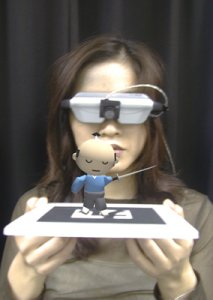
\includegraphics[width=0.3\textwidth]{images/fiducial_marker.png}
\caption{Fiducial marker used to represent a three-dimensional model over it \cite{artoolkit}}
\label{fig:fiducial_marker}
\end{figure}

However, besides requiring human interference on the scene, there situations where the usage of fiducial markers is not possible, feasible or comfortable for the target model. That is the case, for example, of medical applications on which this model is a patient. It's also possible to cite other limitations of fiducial markers, like, for example, occlusion (a virtual image could be not projected if the marker is not completely visible) and illumination (the intensity of light reflected by the marker could make it hard to be identified). Less common, there are approaches that replace fiducial markers \cite{carmigniani} \cite{gallo09} by GPS, gyroscopes, accelerometers, cameras, among others \cite{azuma} \cite{azuma01}. These approaches have the advantage of not requiring human interference on the scene (to put a marker or to move it around).

Depending on the way that a user sees the mixed world, augmented reality can be classified on two ways. When the user sees the mixed world pointing his eyes straight to the real positions with optical scene or video, this augmented reality is called \textit{immersive} or of \textit{direct vision}. On the other hand, when the user sees the mixed world by some device, like a monitor screen or projector, not aligned with the real positions, this augmented reality is \textit{non-immersive} or of \textit{indirect vision} \cite{tori2006fundamentos}.

This work proposes a multi-view environment for augmented reality, of direct vision, composed by two Kinects \cite{kinect} and augmented reality glasses, that allows an observer visualize, in real time, virtual images merged with real images from the target model, transformed to his viewpoint. In this approach, it's not intended to use any fiducial marker. Instead, it will be used a geometric approach based on the data captured by each Kinect. This proposed environment can be used, for example, on the medical field (real situations, education and training) or in other situation where a multi-view environment for markerless augmented reality is applicable. 

\section{Objectives}

The environment proposed on this work aims to contribute to augmented reality applications where virtual images need to be merged with real images in real time, without using fiducial markers, and considering the viewing angle of the observer and the position of the target object.

\subsection{Features}

Based on the study of related works, it was defined the following features that define the scope of the first version of the augmented
reality environment, graphically represented on Figure \ref{fig:diagram}:

\begin{figure}
\centering
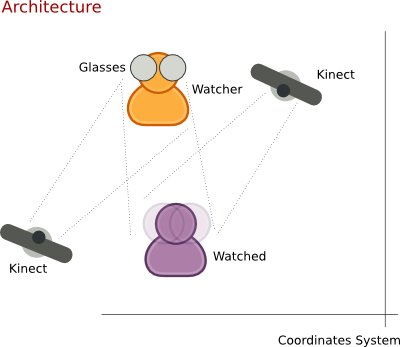
\includegraphics[width=0.8\textwidth]{images/diagram.png}
\caption{Global vision}
\label{fig:diagram}
\end{figure}

\begin{itemize}
  \item There are two main elements on the environment, the observer and the target model;
  \item Observer and target model are positioned one in front of the other, with some restriction of minimum and maximum distance;
  \item The observer sees the combination of a real image with a pre-defined virtual image over the target model, through the augmented
        reality glasses;
  \item The observer and target model can move their heads, in a way that the virtual image adapts itself in real time to fit the new
        viewing angles;
  \item No fiducial marker is used.
\end{itemize}

The elements presented on this environment are the following:

\begin{itemize}
  \item Observer - He is the user of the system that wears a pair of augmented reality glasses and is positioned in front of the target model (which can be a human being, for example, or a static object). On a medical context, the observer would be a medical specialist, responsible for observing the patient and responsible for analyzing the combination of the real image (part of the patient body) with a virtual image (from magnetic resonance imaging or computed tomography). The observer is able to move his head.
  \item Augmented reality glasses - The augmented reality glasses are wore by the observer and have two cameras. The images captured from the target model will be merged with virtual images and displayed on the two lenses of these glasses. On one of the approaches implemented by this work, the observer motion is determined from sensors present on the glasses: accelerometer, magnetometer and gyroscopes. Based on sensor data, it's possible to determine the variation on the orientation of the glasses, and so it's possible to know how much the observer has moved his head. This calculation returns values that define motion on longitudinal axis, vertical axis and lateral axis. The virtual image should be reprojected in real time according to those movements.
  \item Target model - The target model (a human being, for example), is placed in front of the observer and doesn't use any kind of fiducial marker. The main goal is that the virtual image is placed over the target model. In order to calculate where and how the virtual image should be displayed, it's necessary to identify the position and orientation of the real object relative to the observer. This is done based on two sensors placed on the environment, where the first one captures data from the observer and the second one captures data from the target model.
  \item Sensors - Two sensors are placed on the environment and capture data from the observer and the target model (one for each). The information captured by the target model's sensor contains its model, that will be merged with the virtual image.
\end{itemize}

Each device presented on this multi-view (glasses and sensors) environment has its own coordinate system, but all information must be converted to a global coordinate system.

Since there are two sensors and one pair of augmented reality glasses, another objective is to implement two different approaches: one that
uses the augmented reality glasses to determine the observer's pose (based on data from accelerometer and magnetometer) and another one that uses a second Kinect device to determine the observer's pose based on a reconstruction of his model.

\section{Thesis overview}

The next chapter "Conceptual primer" describes some basic theory needed. It also describes the hardwares that are used by this work and how to calibrate them. After that, the "Related work" chapter presents some works related to this one, divided by subject. The third chapter, "Solution architecture", after the theory and related works were presented, explains the steps performed in order to implement the objectives of this work. The results of this implementation are presented on the chapter later, "Results", and finally the conclusions about those results are presented on the last chapter, "Conclusions", where possible future works are also listed.

\xchapter{Conceptual primer}{In this chapter I present the main concepts behind this work.}
\section{Augmented reality}

Augmented reality was born on the decade of 1990, to merge a virtual image or virtual environment with a real image or real environment. But only from the 2000s it became more popular, due to lower costs of hardware and software devices, and ready to be used on tangible and multimodal (voice, touch, gesture, etc.) applications \cite{paddle}. It can be considered the mixing of real and virtual worlds at some point of the continuum reality-virtuality, that connects completely virtual environments to completely real environments \cite{milgram94}, like shown on Figure \ref{fig:cont}. It can also be considered a system that completes the real world with virtual objects, in a way that they seem to exist on the same space, respecting the following features:

\begin{figure}
\centering
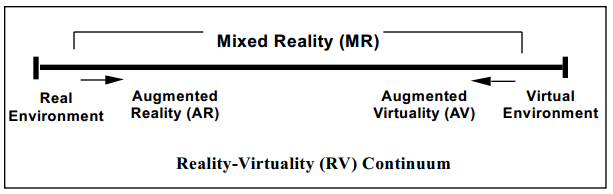
\includegraphics[width=0.5\textwidth]{images/cont.png}
\caption{The augmented reality is localized between the extremes of the reality-virtuality continuum}
\label{fig:cont}
\end{figure}

\begin{itemize}
  \item Real objects are mixed with virtual objects;
  \item Execution is interactive and on real time;
  \item Virtual and real objects are aligned;
  \item Applicable to all human sensory systems, including auditory, olfactory and somatosensory \cite{azuma01}.
\end{itemize}

A typical augmented reality system, that uses a single RGB video feed for tracking and displaying, has basically four steps on its pipeline, as shown on Figure \ref{fig:arpipeline}: camera calibration, video acquisition, tracking and registration, and rendering.

\begin{figure}
\centering
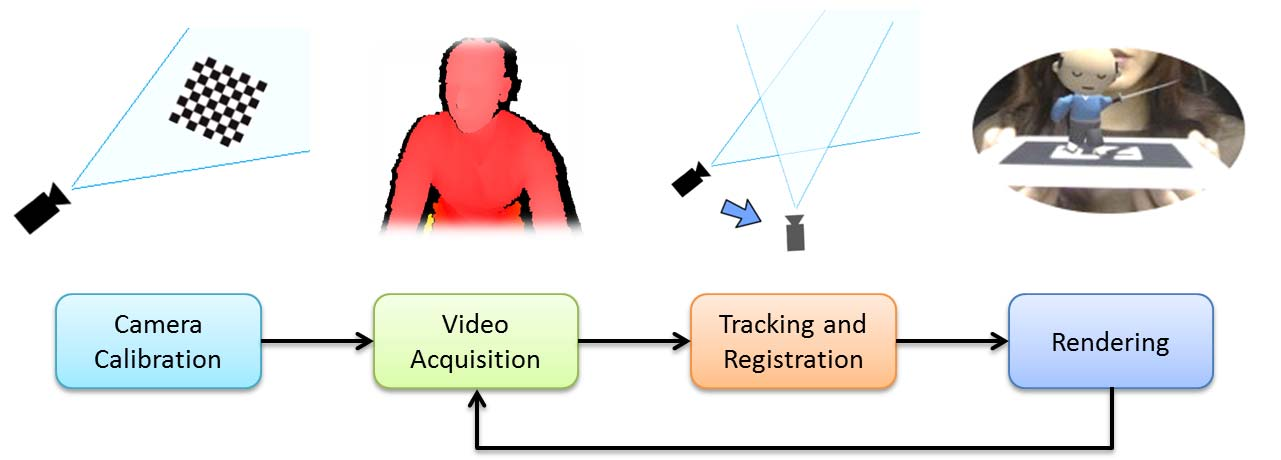
\includegraphics[width=1\textwidth]{images/arpipeline.png}
\caption{The typical pipeline of an augmented reality application \cite{gallo11}}
\label{fig:arpipeline}
\end{figure}

From a human-computer interaction perspective, the augmented reality can be considered a new way of interaction between humans and computers, and, on this aspect, it can be classified as direct vision or indirect vision.

\subsection{Direct or indirect vision}
\label{sec:dirind}

Augmented reality is classified as \textit{direct vision} or \textit{immersive} when the user sees the mixed world pointing his eyes straight to the real position of the objects of interest, like shown on Figure \ref{fig:direct}.

\begin{figure}
\centering
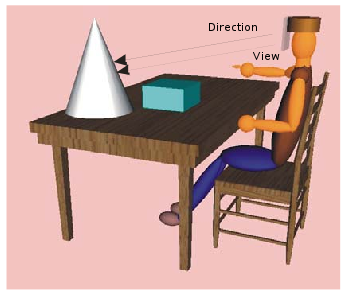
\includegraphics[width=0.5\textwidth]{images/direct.png}
\caption{Immersive augmented reality}
\label{fig:direct}
\end{figure}

On the direct vision, images from the real world can be seen with the naked eye or brought by video, while the generated virtual images can be projected on the eyes, on the real scenario or mixed with the real world video. Immersive augmented reality can be implemented with optical helmets, for example \cite{tori2006fundamentos}.

\begin{figure}
\centering
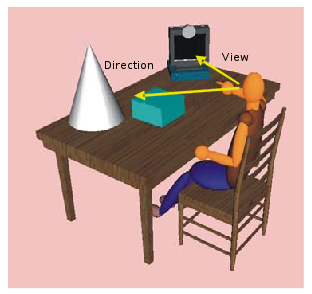
\includegraphics[width=0.5\textwidth]{images/indirect.png}
\caption{Non-immersive augmented reality}
\label{fig:indirect}
\end{figure}

On the other hand, non-immersive augmented reality (indirect vision), happens when the user sees the mixed world through other output device, like a monitor screen, for example, not aligned with the real positions, as shown on Figure \ref{fig:indirect}. On this kind of vision, real and virtual images are merged and displayed as video to the user. It can be achieved by using cameras and projectors \cite{tori2006fundamentos}.

\subsection{Markers}

In order to identify the position where a virtual image should be rendered, two main approaches can be applied by augmented reality applications: one is to use fiducial markers, the other is not use them.

\subsubsection{Fiducial markers}

Fiducial markers are often implemented as square white cards with a black symbol printed (or drawn) on it, easy to be recognized, working like a barcode or QR code. Computer vision techniques are used to calculate the position of the real camera and its orientation relative to the markers, in a way that virtual objects can be projected over them.

Fiducial markers can assume other shapes besides a square card. The Figure \ref{fig:sticker} shows an example of a fiducial marker used on medical applications, similar to a sticker, which is fixed on the patient's skin. On these applications, augmented reality can be used for visualization and training on surgeries. It's possible to collect patient's data in real time, by using non-invasive sensors as the ones used for magnetic resonance imaging and computed tomography. This dataset can be merged in real time with the real image of the patient \cite{azuma}.

\begin{figure}
\centering
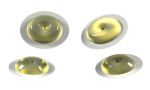
\includegraphics[width=0.5\textwidth]{images/sticker.png}
\caption{Example of fiducial marker used by medical applications}
\label{fig:sticker}
\end{figure}

On motion capture systems, other kinds of markers can also be used, like, for example, the one described on \cite{4526681} and represented on Figure \ref{fig:helmet}. In order to estimate the pose, it uses a single camera and three spherical fiducial markers, which are also reflexive. Two of those markers are placed at the left and right sides of the actor, perpendicular to his ears. The third marker is placed on the same height as the other two, but in front of the actor. The markers have a color close to orange for high reflectance (in order to be easily recognized) and are supported by a structure made of carbon fiber (which is light).

\begin{figure}
\centering
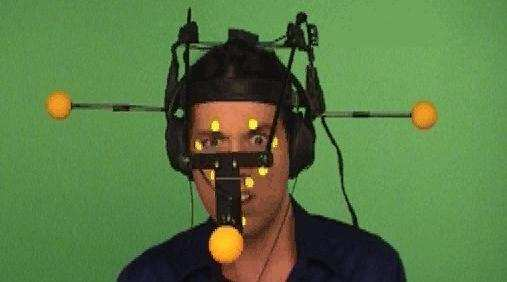
\includegraphics[width=0.5\textwidth]{images/helmet.png}
\caption{Example of fiducial marker for motion capture}
\label{fig:helmet}
\end{figure}

Disadvantages of fiducial markers are listed on \cite{dolz}, for example, they are invasive (need to be placed on the scene or fixed on the target object), they have limited interaction (can't be moved around so much because it needs to still be visible and recognizable) and need to be printed or drawn before using and stored for future usage.

\subsubsection{Markerless}

Markerless augmented reality means that fiducial markers are not used on the scene. Instead, features from the target scene need to be used in order to estimate the camera pose and objects orientations.

Target detection based on computer vision has been extensively studied and successfully applied on augmented reality applications. On related computer vision literature, geometric primitives can be used for pose estimation, on most cases, points, segments, lines, edges of edge points, cones, cylinders, or a combination of two or more of those features.

Markerless augmented reality has the advantage of using parts of the real environment as targets and can even extract information from the environment to be used by the augmented reality system \cite{dolz}.

Avoiding markers leads to a much more effective augmented reality experience, but requires the implementation of several image processing or sensor function techniques, resulting in more complex algorithms and in higher computational resources \cite{shumaker2011virtual}.

\section{Cameras}

Many tasks on augmented reality deal with an imaging device. Usually this imaging device is a camera, which performs a mapping from a 3D world to a 2D image \cite{hanning2011high}. The problem called \textit{camera calibration} is the one that handles the determination of the parameters for this mapping.

\subsection{Calibration}

Camera calibration is a necessary step in 3D computer vision in order to extract metric information from 2D images. Much work has been done, by both the photogrammetry community and the computer vision community. Those techniques can be divided roughly into two categories: photogrammetric calibration (performed by observing a calibration object whose geometry in a 3-D space is known with very good precision) and self-calibration (does not use a calibration object, just move the camera in a scene and get its parameters) \cite{zhang2000flexible}.

Camera calibration means to determine the camera model parameters which fit best to the observed behavior of the actual camera \cite{hanning2011high}. So, it's necessary to measure the distance of an observation to a given camera model. The determination of the optimal camera mapping concerning each of these distance functions defines a non-linear optimization problem, and as such, it depends on the initial value.

Ordinary cameras are very often modelled as pinhole cameras. A pinhole is an imaginary wall with a tiny hole in the center that blocks all rays except the ones that pass through this tiny center hole \cite{bradski2008learning}. Unfortunately, a real pinhole is not a good way to make images because it does not gather enough light for rapid exposure. This is why human eyes and cameras use lenses to gather more light than what would be available at a single point. This way, the simple geometry of the pinhole camera model is not enough and it also introduces distortion of the lens itself.

The camera coordinate system (CCS) is a Cartesian coordinate system defined by the principal plane: The x-axis and y-axis of the CCS determine the principal plane, the z-axis is given by the optical axis. The optical center of the lens determines the origin (0, 0, 0) of the CCS. Thus, in the camera coordinate system, the principal plane becomes ${ z = 0 }$ \cite{hanning2011high}.

Camera calibration is usually split up into two distinct parts, the intrinsic and extrinsic parameters, which will be covered on the following section.

\subsection{Parameters}

The process of camera calibration gives us both a model of the camera's geometry and a distortion model of the lens. Both compose the intrinsic parameters of the camera.

\subsubsection{Intrinsic parameters}

The intrinsic parameters are those that describe the internal geometry of the camera and consist of the focal length, the location of image center in pixel space, the pixel size in the horizontal and vertical directions and radial and tangential distortions \cite{malik2002}. These values are needed to help to describe imperfections in the lens of the camera and give a mapping from camera reference frame to the image plane. The intrinsic parameters depend only on the camera itself, and so they just need to be found once, regardless the environment changes or not (no need for recalibration due to environmental changes). The location of the image center and the pixel size make it possible to link image coordinates $(x_{im}, y_{im})$ in pixels, to the respective coordinates $(x, y)$ in the camera coordinate system \cite{malik2002}:

\begin{center}
$x = -(x_{im} - o_x)s_x$
$y = -(y_{im} - o_y)s_y$
\end{center}

Where $(o_x, o_y)$ define the pixel coordinates of the principal point and $(s_x, s_y)$ define the size of pixels in the horizontal and vertical directions, respectively.

\subsubsection{Extrinsic parameters}

The extrinsic parameters, on the other hand, represent the viewpoint of the camera by a rigid transformation, which describes its position and orientation \cite{bajramovic2010self}. This part of the model is independent of the camera itself. The according parameters are called extrinsic, as they describe the relation between the camera and the world.

According to \cite{tillapaugh2008indirect}, the extrinsic parameters are those that are dependent on the environment. To relate an object's coordinate system to the world's coordinate system, a translation and a rotation matrix are needed. Therefore, the extrinsic parameters consist of these two matrices, so that a mapping from the world coordinate system to the camera reference frame can be found. Since the extrinsic parameters for the camera explain how the camera relates to the environment, if the camera changes position, the parameters have to be recalculated (differently from the intrinsic parameters as explained on the previous section).

The relation between world coordinate system and the camera reference frame can be described by the equation:

\begin{center}
$X_c = R_c \times X + T_c$
\end{center}

Where $X$ is a 3x1 vector that represents a point on the world coordinate space, $R_c$ is the extrinsic rotation matrix, $T_c$ is the extrinsic translation matrix and $X_c$ is a 3x1 vector in the camera reference frame. The rotation matrix is build from the combination of three single-axis rotation matrices:

\begin{center}

$R_{x}(\theta) =
\begin{bmatrix}
1 & 0 & 0 \\
0 & cos(\theta) & sin(\theta) \\
0 & -sin(\theta) & cos(\theta) \\
\end{bmatrix}$

\vspace{10mm}

$R_{y}(\phi) =
\begin{bmatrix}
cos(\phi) & 0 & -sin(\phi) \\
0 & 1 & 0 \\
sin(\phi) & 0 & cos(\phi) \\
\end{bmatrix}$

\vspace{10mm}

$R_{z}(\omega) =
\begin{bmatrix}
cos(\omega) & sin(\omega) & 0 \\
-sin(\omega) & cos(\omega) & 0 \\
0 & 0 & 1 \\
\end{bmatrix}$

\end{center}

The rotation matrix $R$ has the property that its inverse is its transpose, hence $R^TR = RR^T = I$, where $I$ is the identity matrix consisting of 1s along the diagonal and 0s everywhere else.

The translation vector $T$ is how it's possible to represent a shift from one coordinate system to another system whose origin is displaced to another location; in other words, the translation vector is just the offset from the origin of the first coordinate system to the origin of the second coordinate system \cite{bradski2008learning}. So, in order to shift from a coordinate system centered on an object to one centered at the camera, the appropriate translation vector is simply $T = origin_{object} - origin_{camera}$. Thus, a point in the object (or world) coordinate frame $P_o$ has coordinates $P_c$ in the camera coordinate frame: $P_c = R(P_o - T)$.

The extrinsic parameters can be represented by a final matrix called \textit{homogeneous matrix}. It looks as follows:

\begin{center}
$\begin{bmatrix}
R & t \\
0 & 1 \\
\end{bmatrix}$
\end{center}

So, in order to convert from a world origin coordinate to a camera orientation coordinate system, only a single homogeneous matrix needs to be used.

\subsection{Calibration approaches}

There are multiple ways to calibrate cameras. The most common way to perform the calibration is to have multiple points that have known relationship to each other in the world's coordinate system captured in an image from the camera \cite{tillapaugh2008indirect}. As explained previously, for the intrinsic parameters it does not matter how the points are related to the world coordinates, it's only important how they relate to each other. Such parameters consist of the horizontal and vertical focal lengths and the principal point of the camera and the skew. The skew is generally assumed to be zero \cite{furht2011handbook} for many cameras.

Various techniques were created to obtain accurate mappings, including vanishing points for orthogonal directions and calibration from rotation purely \cite{Medioni:2004:ETC:993884}, features extraction which can be lines or points, single-image or multiple-images configurations, different camera models, linear and non-linear algorithms, among many others \cite{Armangue00acomparative} \cite{clarke98}. Self-calibration is indeed feasible with simple image correspondences among frames, yet the participation of control points produces more robust calibration results, in closer agreement with object space constraints \cite{Douskos_automaticcalibration}.

The works by \cite{Tsai86} and \cite{zhang2000flexible} are extensively referenced and propose closed form solutions for the estimation of intrinsic and extrinsic parameters using 3D and 2D calibration patterns respectively. Camera calibration is a much discussed topic but the lack of robust algorithms for features detection makes harder the construction of automatic calibration process \cite{gustavo}. Calibration pattern recognition is a hard task, where the lighting problems and high level of ambiguities are the principal challenges. For this reason, the algorithms often require user intervention for a reliable detection of the calibration points.

There are some tools available for automatic camera calibration. Two of the most popular ones are The Bouguet MatLab Toolbox \cite{matlab} and the OpenCV library \cite{opencv}. The former is an application that asks the user to define four extreme points that represent the area where an algorithm searches for the calibration points, given the number of rows and columns of the pattern. The latter is a very popular computer vision library that offers an automatic way to detect chessboard patterns in images by the \textit{findChessboardCorners()} function. The method performs successive morphological operators until a number of black and white contours are identified, subsequently the corners of the contours make up the calibration point set. The pattern is recognized only if all rectangles are identified. Figure \ref{fig:chessboard} shows how a person can use a chessboard in order to calibrate a camera using the OpenCV library.

\begin{figure}
\centering
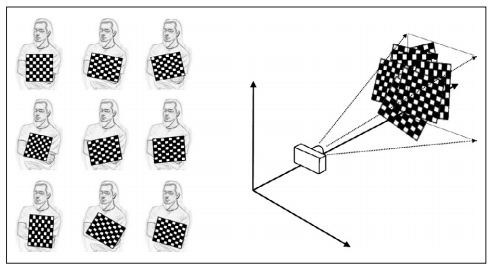
\includegraphics[width=0.5\textwidth]{images/chessboard.png}
\caption{Images of a chessboard being held at various orientations (left) provide enough information to completely solve for the locations of those images in global coordinates (relative to the
\label{fig:chessboard}
camera) and the camera intrinsics \cite{bradski2008learning}}
\end{figure}

As stated by \cite{arca}, the well-known algorithms for chessboard detection proposed by \cite{Tsai86} and \cite{zhang2000flexible} can achieve good calibration results since both of them are based on an initialization procedure that requires the precise corners positions of a calibration pattern (a chessboard, for example). Although the pattern to be detected is generally a simple object, the detection of its corners at sub-pixel precision is a very difficult task to be solved under uncontrolled acquisition conditions. At the state of art, most of the presented methods determine the positions of the chessboard corners by means of a two step processing scheme. At first the corners are detected with pixel precision, by means of edge detection methods; to increase the detection accuracy, the second step modifies their positions by the interpolation of the found borders. Those methods rarely reach a high accuracy, since the interpolation provides just a guess about the precise corners positions. Some authors try to improve the accuracy in the later steps of camera calibration, which increases computational cost, while others, like \cite{arca}, does not make any assumption on the orientation and scale of the chessboard and try to first find the chessboard, then determine the size of the squares and later on find the corners by using a simple statistical model.

\subsection{Multi-view}

Calibrating a multi-camera system accordingly means estimating the intrinsic and extrinsic parameters of all cameras \cite{bajramovic2010self}. Actually it is mainly concerned with estimating extrinsic parameters, since most approaches first compute intrinsic parameters individually for each camera. Extrinsic parameters are subsequently estimated given the intrinsic parameters.

The calibration task is usually formulated such that the world coordinate system may be chosen arbitrarily, which amounts to calibrate up to a rigid transformation of the whole system. Furthermore, if no metric measurements are used, the scale of the multi-camera system cannot be determined. This is the case if only correspondences between the cameras are used as input (of the extrinsic calibration) \cite{bajramovic2010self}.

According to \cite{hanning2011high}, the calibration of a stereo camera system is more than calibrating two camera separately: An additional constraint for the stereo camera system can be applied, since a calibration target is observed by both cameras.

So, in theory, calibration of a multi-camera system is possible by individually calibrating intrinsic and extrinsic parameters of all cameras involved with respect to the same world coordinate system using classical calibration methods. This just requires that all cameras observe a common calibration object or that a calibration object is moved to precisely known positions such that every camera can observe it. The first approach imposes very strict limitations on the allowable relative camera poses (relative orientation and position) or requires a very large calibration object, which is generally complicated \cite{Chen00widearea}.

Once cameras are calibrated, they are ready to register objects from a mixed reality scene. In general, traditional methods can be classified into three types: sensor-based methods, image-based methods and hybrid methods \cite{shumaker2011virtual}. The first two will be covered in the next sections; the third, which is also applied by this work, won't be covered here since it's basically a combination of the first two methods.

\section{Sensor-based registration approach}

Three-dimensional (3D) reconstruction of an environment is an important problem that has received much attention in past decades. It can be defined as the process of capturing the shape and appearance of real objects \cite{chandra20123}. Recovering 3D surface structure of an object has been a central issue in computer vision, however due to high precision requirements of the registration process, no sensing device, alone, in the past, has achieved the results required by most augmented reality applications \cite{vall98}. But on the last years, with the launch of inexpensive RGBD sensors (notably the Kinect), applications based on sensor registration became cheaper and more feasible. In the past, most augmented reality applications relied on sensors, such as magnetic, mechanical or inertial, but on the next sections only the Kinect will be covered.

\subsection{Kinect}
\label{sec:kinect}

Kinect \cite{kinect} is a new and widely-available sensor platform that incorporates a structured light based depth sensor. It can be classified as an RGB-D camera, since it comes with not only an RGB camera, but also a depth sensor. While the quality of this depth map is generally remarkable given the cost of the device, a number of challenges still remains \cite{kinfu2}: the depth images can contain a number of "holes", when depth reading was not possible, due to certain materials or scene objects that don't reflect infra-red (IR) light, very thin or small structures or surfaces at glancing incident angles. Data can also be missed if the device is moved fast.

The depth sensing system of Kinect consists of two parts: the IR laser emitter (which creates a known noisy pattern of structured IR light) and the IR camera. The depth sensing works on a principle of structured light. There's a known pseudo-random pattern of dots being pushed out from the camera. These dots are recorded by the IR camera and then compared to a known pattern \cite{hackingkinect}. The disturbances are known to be variations in the surface and can be detected as closer or further away. The fact that light matters brings three main problems:

\begin{itemize}
  \item The wavelength must be constant (Kinect handles it internally)
  \item Ambient light can cause issues
  \item Distante is limited by the emitter strength
\end{itemize}

Within the sensor, there is a small heater/cooler that keeps the laser diode at a constant temperature. This ensures that the output wavelength remains as constant as possible, given variations on power and temperature. Ambient light is the bane of structured light sensors, but there are measures to mitigate this. One is an IR-pass filter that prevents stray IR in other ranges from blinding the sensor. However, Kinect doesn't work well in places with strong sunlight. Sunlight's wide band IR has enough power on Kinect's IR sensor range in order to blind it \cite{hackingkinect}.

The RGB camera collects 30 frames per second of actual real time events at a 640x480 resolution \cite{kinecthacks}. The Kinect also has the option to switch the camera to high resolution, running at 15 frames per second (fps), which in reality is more
like 10 fps at 1280x1024 pixels. Of course, the former is reduced slightly to match the depth camera;
640x480 pixels and 1280x1024 pixels are the outputs that are sent over USB. The camera itself possesses
an excellent set of features including automatic white balancing, black reference, flicker avoidance, color
saturation, and defect correction \cite{hackingkinect}.

The Kinect is calibrated at factory and has built in numbers for converting the disparity values to depth values, and also for mapping 3D points to the color camera. However, the calibration from factory uses a simple model where depth values are fast enough to be computed, but its accuracy can be improved by using other calibration methods \cite{magnus2013}.

One of those method is the one by \cite{burruscal}. It's a same-automatic way to calibrate the Kinect depth sensor and the RGB output to enable a mapping between them. It's based on a standard stereo calibration technique but the main difficult comes from the depth image that is not able to detect patterns on a flat surface. So, the pattern is created using depth difference. On the first step, the color camera intrinsics are calibrated using standard chessboard recognition. In order to get the intrinsic parameters for the depth camera, the corners of the chessboard on the depth image are extracted and stored (by hand). The raw depth values are integers between 0 and 2047, which can be transformed in meters using some fixed internal values from Kinect, as shown on the following algorithm:

\begin{algorithmic}
\Function{raw\_depth\_to\_meters}{$raw\_depth$}
\If {$raw\_depth \leq 2046$}
\Return $1.0 / (raw\_depth * -0.0030711016 + 3.3309495161)$
\Else \Return $0$
\EndIf
\EndFunction
\end{algorithmic}

Stereo calibration can also be performed by just selecting the corners of the chessboard on the color images. Depth pixels can be mapped to color pixels by undistorting RGB and depth images using the estimated distortion coefficients and then using a formula to project each pixel of the depth camera to metric 3D space.

All the information gathered by the RGB camera and the IR camera are available in two data streams provided by Kinect. One data stream makes it possible to build an RGB map and the other data stream makes it possible to build a depth map. Both maps without any calibration are useless, so it's necessary to perform a calibration called \textit{depth registration} in order to get the correspondences between a pixel on the RGB map with another pixel on the depth map, which can be done by software but using built-in data stored on Kinect's firmware.

\subsection{Registration}

The depth maps generated by the Kinect contain discrete range measurements of the physical scene, thus this data can be reprojected as a set of discrete 3D points (or point cloud). Point clouds are sets of data containing collections of 3D vertices, often derived from an observation of a real world scene \cite{price2012}. At a first glance, point clouds can be divided into two main classes: unorganized or organized. If the dataset is organized, it can be directly indexed or searched in a tree-basis in order to find an specific point and also its neighbors. This is very important because most of the point clouds operations depends on being able to compute properties of a point based on its neighborhood (or k-closest points). So, an unorganized point cloud should be first parsed into a tree structure in order to allow faster computations. This tree structure can be, for example, an array, an octree or a KD-tree.

Once a point cloud is organized, operations can be performed over it. Measure error is expected in any conversion from the real world to a digital structure. As stated previously, variations on the surface or scene objects materials or shapes, lighting, edges, among others, can lead to noisy point clouds, giving an inaccurate result. The next sections will cover three common operations over point clouds.

\subsubsection{Filtering}

So, filtering is one of the first tasks to be performed over an early fetched point cloud. There are many filtering algorithms for this, but one of most powerful ones is the statistical outlier filter, which can solve these irregularities by performing a statistical analysis on the neighborhood of each point, and by discarding the ones that don't meet an specific criteria. In the one implemented by the Point Cloud Library \cite{pclstatout}, the outliers removal is based on the computation of the distribution of points to neighbors distances in the input dataset. For each point, the mean distance from it to all the neighbors is computed, and by assuming that the resulted distribution is Gaussian (with a mean and standard deviation), all points whose mean distances are outside the interval defined by the global distances mean and standard deviation can be considered outliers and removed from the dataset.

\subsubsection{Normal estimation}

The normal vector, often simply called the "normal" to a surface is a vector perpendicular to it \cite{normalwolf}. Given a geometric surface, this is easy to be determined, however, this is not straightforward for point clouds, where estimation is necessary. Normal estimation at a point is an important task in order to determine whether points are part of the same object. There are many different methods for normal estimation, and one of the simplest ones is the one that approximates this problem by the problem of estimating the normal of a plane tangent to the surface, which becomes a problem of estimating the least-square plane fitting \cite{pclnormal}. Therefore the problem is reduced to an analysis of eigenvalues and eigenvectors of a covariance matrix generated from the nearest neighbors of the target point. Another simple method, given a point and its neighborhood, is to just average the normals created from the cross products of the vectors to all of the other points on the neighborhood \cite{price2012}.

\subsubsection{Segmentation}

Segmentation is the process that separates a set of points into the different objects that they represent. For example, if the point cloud is acquired from a room, the segmentation would determine which sub-sets of points from this point cloud represent a chair, a desk, and any other object present in the captured room. Approaches for this include derivative computation of the normal field (in order to determine when one object ends and another starts) or even pattern matching.

On Kinect, these operations can be performed in the following way:

\begin{itemize}
  \item Each point $P$ at position $(m, n)$ on the point cloud can be computed by $P_{m, n}(t) = D_{m, n}(t) \times K_{m, n}$, where $D$ is the depth array given by Kinect and $K$ is the intrinsic field-of-view tensor;
  \item Normal vector at any point $(m, n)$ is an approximation of $(P_{m+1, n} - P_{m,n}) \times (P_{m, n+1} - P_{m,n})$;
  \item Segmentation can be done based on color values (from RGB map) or depth values (from depth map)
\end{itemize}

Two consecutive point clouds, scanned at different times, can be aligned in order to calculate the transformation of the captured object.

\subsection{Alignment}
\label{sec:icp}

There also many methods for aligning two point clouds, but the Iterative Closest Point (ICP) \cite{icp} is far the most implemented one, proposed on 1992 for the registration of 3D shapes, but it's also used to reconstruct surfaces of different scans, gather optimal path planning, and so on. The main goal of the algorithm is to minimize the difference between two point clouds, one called the \textit{target} and another one called the \textit{source}. The target point cloud is kept fixed, while the source point cloud is transformed in order to best match the fixed target point cloud. The algorithm iteratively revises the transformation (composed by rotation and translation) in order to minimize the difference between the source point cloud and the target point cloud, until it reaches a local minimum.

On this context, the interest is on applying the algorithm to point sets, however it was originally designed to also work with six other structures: line segment sets, implicit curves, parametric curves, triangle sets, implicit surfaces and parametric surfaces \cite{hajnal2014medical}.

The algorithm has only two stages, and then iterates. On the first stage, the closest target point for each source point is identified. The second stage tries to find the least square rigid body transformation that relates these two point sets. The algorithm then iterates to redetermine the closest point set and continues until it reaches the local minimum match between the source and target surfaces, as determined by some threshold.

Regardless the representation of the source surface $P$, it is first converted to a set of points ${p_i}$. The target data remains in its original representation. As explained, the first stage means identifying the closest point on the target surface $T$ for each point $p_i$ on the source surface $P$. This is the point $x$ in $T$ where the distance between $p_i$ and $x$ is minimum:

\begin{center}
  $d(p_i, x) = min_{x \in T} \Vert x - p_i \Vert$
\end{center}

All the closest points (one for each $p_i$) are returned as new a set ${q_i}$. A least squares registration between the points $p_i$ and $q_i$ can be performed and so the set of source points $p_i$ can be transformed to a set of points $p'_i$ using the rigid body transformations (composed by a rotation and a translation) that was calculated, and then the closest points can be identified again. The algorithm stops when the change in mean square error between two iterations goes below a threshold. Since the algorithm iterates to a local minimum closest to the starting point, it may not find the best solution, that's why the original authors propose to start the algorithm multiple times and then choose the minimum of the minima obtained \cite{icp}.

The algorithm can be optimized by storing the solutions at each iteration, for example. Actually many variations were proposed to the original version, mainly focused on performance improvements, like using KD-trees \cite{zhang1994}, Lie group representation \cite{Dong201467} or expectation maximization estimation for point set registration with noise \cite{6957732}.

\subsection{Reconstruction}
\label{sec:kinfu}

KinectFusion \cite{kinfu} \cite{kinfu2} is probably the most famous algorithm for reconstructing objects using the Kinect device. It is the state-of-art algorithm for real-time reconstruction and rendering of a real world scene, and is implemented on the PCL \cite{pcl} library under the name of KinFu. In order for this implementation to work, a powerful processor and a graphics card with a CUDA-enabled Nvidia GPU are required, so it can run at at least 30 frames per second.

The algorithm was originally developed by Microsoft Research in 2011. It allows a user to reconstruct a three-dimensional scene in real-time and with good level of details by just moving the Kinect sensor around the real scene.

The input for the algorithm is a temporal sequence of depth maps as returned by the Kinect device. Since the original algorithm just uses depth maps and doesn't use any color information from the RGB sensor, it can in theory work in a completely dark environment. It runs in real-time, so it proceeds by using a frame per time as provided by the depth sensor. A surface representation is extracted from the current depth frame and a global model is refined by first aligning and then merging the new surface with it. The global model is obtained as a prediction of the global surface that is being reconstructed and refined at each iteration \cite{michele}.

So, at each new frame, the new depth map obtained from the depth sensor is used as input for the algorithm. This depth map must be converted into a three-dimensional point cloud with vertex and normal information. This is done at different, layered resolutions, resulting in a number of images with different levels of details, which is originally defined in the algorithm as three. This is called \textit{multi-resolution pyramid} (see Figure \ref{fig:pyr}), on which the lower resolution layers are obtained by sub-sampling the higher resolution ones.

\begin{figure}
\centering
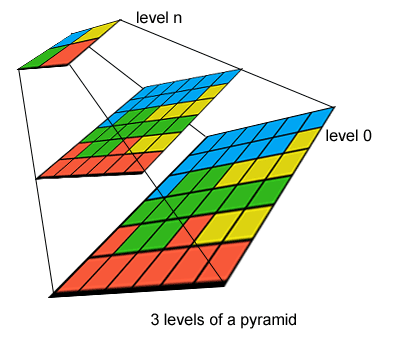
\includegraphics[width=0.5\textwidth]{images/pyr.png}
\caption{A multi-resolution pyramid with three levels \cite{michele}}
\label{fig:pyr}
\end{figure}

The depth map is converted into a three-dimensional point cloud by back-projection. In order to do that, it's used the internal calibration matrix that is stored in Kinect, that matches depth values to actual 3D coordinates. The normal of each point is estimated through cross-product of two vectors: the vector joining the chosen point and the one above it, and the vector that pass through the chosen point and the one at its right. In other words, since the points are arranged as depth pixels, if point $(x, y, z)$ is picked up, points $(x, y+1, z)$ and $(x+1, y, z)$ will be used for normal estimation, where $x$ and $y$ are image coordinates and $z$ is the depth value at these coordinates. At this point, there is a point cloud with normal and vertex information for each point with three distinct levels of details. This cloud is considered ordered since the points are arranged according to the pixels on the depth map.

The next stage is the alignment. The first point cloud is related to the model that was captured. From the second step on, the new point cloud is aligned to the current model and them merged to it in order to produce more refined model through iterative steps. The alignment is performed through the iterative closest point algorithm (ICP). A point-to-point approach is used here: for each point in the current point cloud, the closest one on the previous (global) point cloud is considered, and the distance between them is calculated. The final transformation at the step is the one that minimizes the total error between all point pairs. It's important to notice that KinectFusion doesn't use the standard ICP algorithm since it's too slow to be applied on a real-time context. The difference here is that is assumes that the changes between the current cloud and the previous one are small, which makes sense if the algorithm runs in real-time (for example, at 30 frames per second) and if the Kinect is moved slowly. The modified ICP back-projects the two clouds onto the camera image frame of the model and so they are considered to match if they fall on the same pixel. To make it even faster, the ICP iterations are performed at three resolutions. After a match is found, the modified ICP algorithm calculates the error between two points in a match by using a point-to-plane metric. Some iterations later, the modified ICP will generate a six degrees of freedom transformation matrix, composed by a rotation and a translation, which aligns the source point cloud with the target point cloud.

After that, comes the reconstruction itself. Once the transformation is found and this the current pose of the camera can be estimated, the new cloud is ready to be merged with the current model. In order to avoid losing details, the raw depth data is used instead of the filtered one. This step is based on a Truncated Signed Distance Function (TSDF). What this function does is extract the surface of objects in the scene and assign negative numbers to pixels inside objects or inside an area not yet measured, and positive numbers to pixels outside the surface. For pixels on the surface, this number is zero, for pixels outside the surface, this value is greater for pixels far from the surface and lower for pixels near the surface. TSDF is computed for the new cloud and merged to the current model's TSDF.

On the last step, the resulting TSDF is used to reconstruct the surface of the refined model, which is achieved through ray casting. It is performed from the global camera focal point by intersecting the zero level set of the TSDF. The refined ray-casted model will be used for the next step of the ICP alignment. The end result of the algorithm is a 3D surface representing the acquired scene.

Since the ICP make assumptions about small changes between two point clouds, sudden movements can make it converge to a wrong match, and then break the tracking and consequently the reconstruction. On the other hand, the algorithm is very robust for presence of dynamic objects on the scene, given enough iterations of it. (for example, if a desk is being captured on a room and someone walks in, this person will be removed from the reconstruction). This is due to the weighted average used during merging the TSDFs \cite{michele}.

\section{Vision-based registration approach}

Registration based on sensors relies solely upon geometric information, for example, the spatial coordinates of the points in two clouds. As a result, environments that don't provide high geometric texture (for example, plane surfaces like a wall) can cause sensor tracking to fail. For such cases, a vision-based registration approach can be applied, by using the RGB information from the images \cite{kinectkanade}. 
\subsection{Optical flow}

Optical flow is a pattern that describes the apparent motion of objects, edges or surfaces on a visual scene caused by the relative motion between that object and an observer (a camera or the human eye) \cite{burton1978thinking}. This concept was first introduced by the psychology in order to describe the visual stimulus provided to animals moving on the world \cite{gibson1950perception}.

A fundamental problem in the processing of image sequences is the measure of the optical flow (or image velocity). The main objective is to compute an approximation to the 2D motion field - a projection of the 3D velocities of surface points onto the imaging surface - from spatiotemporal patterns of image density. Once computed, the measurements of image velocity can be used for many purposes, including object tracking \cite{opticalflow}.

The field of optical flow estimation is making big progresses as evidenced by the increasing accuracy of current methods on the Middlebury optical flow benchmark \cite{Scharstein:2002:TED:598429.598475}. After almost 30 years of research, these methods have obtained an impressive level of reliability and accuracy, by combining a data term that assumes constancy of some image property with a spatial term that models how the flow is expected to vary across the image \cite{opticalflow14}.

Differential methods belong to the most widely used techniques for optic flow computation in image sequences. They can be classified into local methods such as Lucas-Kanade technique or Bigun's structure tensor method, and into global methods such as the Horn/Schunck approach and its extensions. Often local methods are more robust under noise, while global techniques yield dense flow fields \cite{lkhs}.

Despite their differences, many of these techniques can be viewed conceptually in terms of three stages of processing \cite{opticalflow}:

\begin{itemize}
  \item Pre-filtering or smoothing with low-pass/band-pass filter in order to extract signal structure of interest and to enhance the signal-to-noise ratio;
  \item The extraction of basic measurements, such as spatiotemporal derivatives (to measure normal components of velocity) or local correlation surfaces;
  \item The integration of these measurements to produce a 2D flow field, which often involves assumptions about the smoothness of the underlying flow field.
\end{itemize}

One of the most popular methods for computing the optical flow of an image is the Lucas-Kanade algorithm, which will be explained on the following section.

\subsection{Lucas-Kanade algorithm}
\label{sec:lucas}

The Lucas-Kanade \cite{lk} algorithm is a differential method for computing the optical flow of an image \cite{kinectkanade}. The goal of Lucas-Kanade is to align a template image $T(x)$ to an input image $I(x)$ where $x = (x, y)^T$ is a column vector containing the pixel coordinates. If the Lucas-Kanade algorithm is being used to compute optical flow or to track an image from time $t = 1$ to time $t = 2$, the template $T(x)$ is an extracted sub-region (a window) of the image at $t = 1$ and $I(x)$ is the image at $t = 2$. Applications of the Lucas-Kanade algorithm range from optical flow and tracking to layered motion, mosaic construction and face coding. Numerous variations has been made to the original algorithm \cite{lk20}.

The basic idea of the Lucas-Kanade algorithm is based on three assumptions \cite{bradski2008learning}:

\begin{itemize}
  \item Brightness constancy: a pixel from the image of an object in the scene does not change in appearance as it (possibly) moves from frame to frame. For grayscale images (although Lucas-Kanade can also be done in color) this means that it's assumed that the brightness of a pixel does not change as it is tracked from frame to frame;
  \item Temporal persistence: the image motion of a surface patch changes slowly in time. In practice, this means the temporal increments are fast enough relative to the scale of motion in the image that the object does not move much from frame to frame;
  \item Spatial coherence: neighboring points in a scene belong to the same surface, have similar motion, and project to nearby points on the image plane.
\end{itemize}

Mathematically, the goal of the Lucas-Kanade is to minimize the sum of squared error between the two images, the template $T$ and the image $I$ warped back onto the coordinate frame of the template \cite{lk20}:

\begin{center}
  $\sum_{x}{[I(W(x;p))-T(x)]^2}$
\end{center}

Where $W(x;p)$ denote the parametrized set of allowed warps, where $p = (p_1,...,p_n)^T$ is a vector of parameters. The warp $W(w;p)$ takes the pixel $x$ in the coordinate frame of the template $T$ and maps it to the sub-pixel location $W(x;p)$ in the coordinate frame of the image $I$. In this context of optical flow computation, the warps $W(w;p)$ are the translations:

\begin{center}
$W(w;p) = \begin{matrix}
          x + p_1 \\
          y + p_2 \\
          \end{matrix}$
\end{center}

Where the vector of parameters $p = (p_1, p_2)^T$ is then the optical flow.

Warping $I$ back to compute $I(W(x;p))$ requires interpolating the image $I$ at the sub-pixel locations $W(x;p)$. The minimization is performed with respect to $p$ and the sum is performed over all of the pixels $x$ in the template image $T(x)$. Minimizing the expression is a non-linear optimization task even if $W(w;p)$ is linear in $p$ because the pixel values $I(x)$ are, in general, non-linear in $x$. In fact, the pixel values $I(x)$ are essentially unrelated to the pixel coordinates $x$. To optimize the expression, the Lucas-Kanade algorithm assumes that a current estimate of $p$ is known and then iteratively solves for increments to the parameters $\Delta{p}$, so the expression is (approximately) minimized:

\begin{center}
  $\sum_{x}{[I(W(x;p + \Delta{p}))-T(x)]^2}$
\end{center}

With respect to $\Delta{p}$, and then the parameters are updated:

\begin{center}
  $p \gets p + \Delta{p}$
\end{center}

These steps are iterated until the estimates for the parameters $p$ converge.

The result of the algorithm is a set of optical flow vectors distributed over the image which give an estimation idea of the movement of objects in the scene, although some of those vectors will be erroneous \cite{raul}.

The Lucas-Kanade method can be applied in a sparse context because it relies only on local information that is derived from some small window surrounding each of the points of interest. The disadvantage of using small local windows in Lucas-Kanade is that large motions can move points outside of the local window and thus become impossible for the algorithm to find, which led to the development of the "pyramidal" Lucas-Kanade algorithm \cite{Bouguet00}, one of many approaches that have been used to improve the convergence rate and reduce the likelihood of falling into a local minimum.

One component in many algorithms is a coarse-to-fine strategy. The most common approach is to build image pyramids by repeated blurring and downsampling. So, optical flow is first computed on the top level (fewest pixels) and then upsampled and used to initialize the estimate at the next level \cite{dblk}, as shown on Figure \ref{fig:plk}. Computation at the higher levels in the pyramid involves far fewer unknowns and so is far faster. The initialization at each level from the previous level also means that far fewer interactions are required at each level. Due to this, pyramid algorithms are usually faster than a single solution at the bottom level.

\begin{figure}
\centering
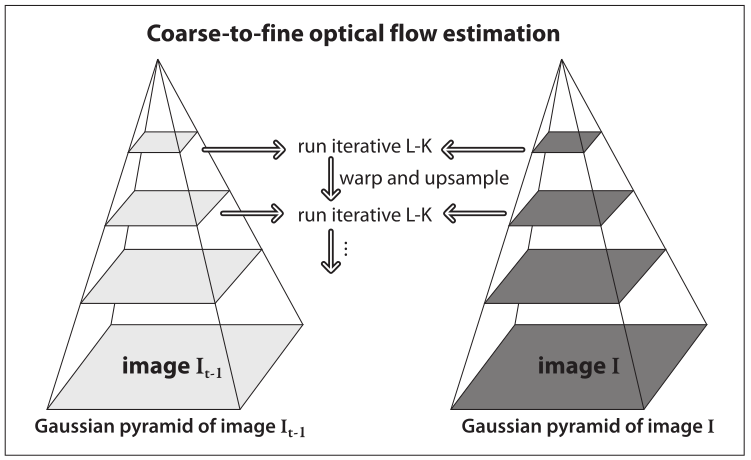
\includegraphics[width=0.5\textwidth]{images/plk.png}
\caption{Pyramid Lucas-Kanade optical flow: running optical flow at the top of the pyramid first
\label{fig:plk}
mitigates the problems caused by violating our assumptions of small and coherent motion; the motion estimate from the preceding level is taken as the starting point for estimating motion at the next layer down \cite{bradski2008learning}}
\end{figure}

The features to be tracked by the Lucas-Kanade algorithm can be manually defined or identified from an algorithm, like the popular one proposed by Shi and Tomasi \cite{shi}, called "good features to track", and implemented by the OpenCV library \cite{opencv}. The idea of this algorithm is a modification of the Harris Corner Detection \cite{harris}, which basically replaces Harris' scoring function. Figure \ref{fig:shi-harris} shows the feature points on the same input image as identified by both algorithms.

\begin{figure}
\centering
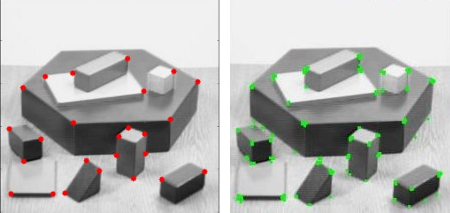
\includegraphics[width=0.5\textwidth]{images/shi-harris.png}
\caption{The same input image being used for features identification by Shi-Tomasi algorithm (red dots) and by Harris Corner Detector (green dots)}
\label{fig:shi-harris}
\end{figure}

So, the Lucas-Kanade algorithm, applied over a good set of feature points, is an efficient method for obtaining optical flow information at interesting points in an image and works for moderate object speeds.

\xchapter{Related works}{In this chapter I present some related works. Since it hasn't been found any work that uses a multi-view markerless augmented reality environment based on hybrid reconstruction, this chapter is divided into subjects related to the this work: usage of multiple Kinects, optical flow, markerless augmented reality, medical applications, multi-view environment, reconstruction, etc.}

\section{Augmented reality applications for medicine}

On the field of augmented reality, one of the first approaches was to track known patterns, that's how much fiducial markers work. The traditional ARToolKit \cite{artoolkit} is probably the most famous of them and augments virtual objects onto black and white square markers. Its advantage is simplicity and performance, since it works also with modest computers and commodity cameras. However, it doesn't support any kind of occlusion, since its fitting process is based on a four-lines approach that requires the marker to be fully visible by the camera.

Augmented reality has been widely implemented on medicine on the last years, for training, simulation, therapy and so on. Many works on this field are based on fiducial markers in order to calculate the camera's real position in relation to the marker's real position, like the system called ARBioMed \cite{arbiomed}. The idea of this system is to represent a virtual, three-dimensional heart over a marker placed on the target user's chest. This virtual heart has its pulsation simulated according to a received signal. From this system, the operator user can define, through a user interface, a fixed pulse rate to be simulated on the heart. In order to set the size of the heart based on the dimensions of the user chest, two other fiducial markers are used, as shown on Figure \ref{fig:arbiomed}. This architecture makes the implementation simpler, since it is based on ARToolKit \cite{artoolkit}, a popular and straightforward framework for augmented reality based on fiducial markers. However, the markers pollute the augmented reality scene and offers a less comfortable experience to the target user, since the markers are invasive.

\begin{figure}
\centering
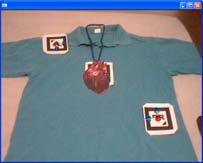
\includegraphics[width=0.5\textwidth]{images/arbiomed.png}
\caption{ARBioMed running, with three fiducial markers \cite{arbiomed}}
\label{fig:arbiomed}
\end{figure}

Another work on the medical field that is based on the traditional square fiducial markers is the motion capture system presented on \cite{fisio}, whose goal is to follow up physiotherapy exercises performed by patients. As shown on Figure \ref{fig:fisio}, fiducial markers are fixed on parts of the patient's body where motion will be captured. Based on trigonometric evaluation of the markers' position, it's possible to establish the range of motion that was executed.

\begin{figure}
\centering
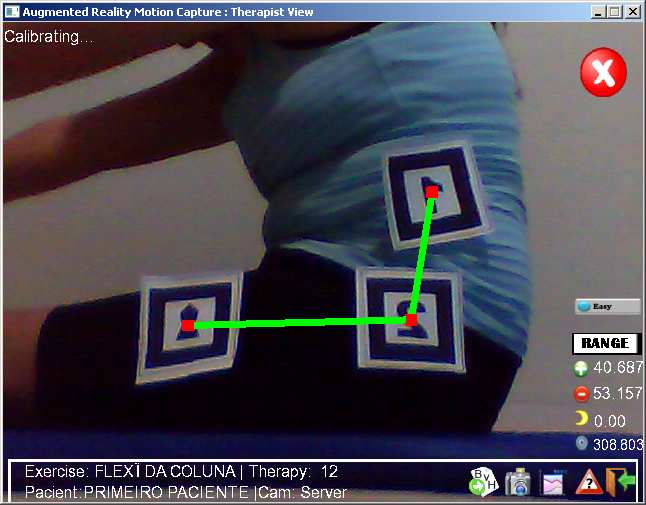
\includegraphics[width=0.5\textwidth]{images/fisio.png}
\caption{User under augmented virtual therapy \cite{fisio}}
\label{fig:fisio}
\end{figure}

Augmented reality applications on medicine are also applied for training, like the ANGELS system \cite{angels}. The main objective of this project is to test the utility of augmented reality to train in prevention of risks at work in the health care sector. After conducting a requirements analysis in order to obtain a general framework for the priority risks in safety at work within the health care, a pilot study was carried out and preliminary results showed a good opinion of the users as well as favorable usability of the system.

Still on training, the work at \cite{endo} implemented augmented reality telementoring platform to overlay the instruments of a mentor onto the trainee's laparoscopic monitor, for surgical training. The study concluded that the designed platform was a more effective training technique in teaching laparoscopic skills to medical students compared to traditional methods, since it reduced the number of failed attempts and resulted in faster suture times.

On the therapy side, there is a work that developed a low-cost spatial augmented reality system that allows individuals with stroke to practice hand and arm movement exercises at home or at a clinic with minimal support of the therapist \cite{stroke}. This setup uses a color marker, fixed on the patient's hand, to track his movement and check how accurate he performs. After that, a score is displayed to him. There are setups for some exercises, and one of them is displayed on Figure \ref{fig:stroke}.

\begin{figure}
\centering
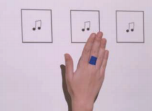
\includegraphics[width=0.5\textwidth]{images/stroke.png}
\caption{Patient with stroke performing an exercise to reach melody boxes \cite{stroke}}
\label{fig:stroke}
\end{figure}

This study of related works on the field of augmented reality applied on medicine showed that most of the works are still based on fiducial markers. Works related to markerless augmented reality approaches will be studied on the next section.

\section{Markerless augmented reality}

On the last years, alternatives to the traditional fiducial markers started to emerge. One of the common problems related to fiducial markers is that the marker needs to be located on the field of view of the camera. A possible solution for this is presented on \cite{5739718}, that is able to track a camera based on plane tracking algorithm. This technique has been applied mainly due to its simple geometry. Results also show that 3D objects can be used on augmented reality applications with primitive-based modeling \cite{KimLW10}.

One of the first works to propose an algorithm for markerless object tracking was \cite{Comport03d}, that suggests a tracking algorithm based on 3D models to calculate the distance between the camera and the objects. Based on this calculation, objects can be placed on the scene. Though this method seemed to be robust on handling occlusion and luminosity issues, which are weak points of the fiducial markers, it still had some limitations. This is an example of an application based on models, that already uses geometric 3D data to identify where to place a virtual image on the real scene.

Other alternatives to fiducial markers are proposed on \cite{wuest}, that uses an adaptive edge detector, \cite{ferrari}, that renders planar textures over planar fragments previously identified, and on \cite{klein}, which proposed a multi-thread system to track a camera and to compute a three-dimensional map of the available marks, using a hand-held camera.

The system designed on \cite{ZhangL12} allows any object from the environment to be used as a marker, instead of using a fiducial marker. Besides that, the system was designed to work with low-contrast surfaces (like human hand marks). In order to place a three-dimensional object, the system uses salient points from the environment combined with a local texture, which turns the detection much more stable.

Like that work, other works show that feature detection on the target scene can achieve good performance. Descriptors are usually computed from key-points of the scene, so, they don't reach great performance when dealing with objects without texture and/or with few key-points on their surfaces \cite{bay}.

On the other hand, object recognition based on depth focuses on geometric properties of the target, like curves or edges. An object can be identified based on its depth map.

\section{Sensors}

Recently augmented reality works use sensors in order to capture scene data and use them for pose estimation, replacing the need for markers. Such sensors can capture real images from the scene in order to identify natural marks or features, or can even capture three-dimensional objects to be used as geometric markers.

The study on \cite{Lee20125286} proposes a cranial augmented reality system which performs image-to-patient registration using only natural facial features. The hardware for this project is composed by three calibrated cameras and no fiducial markers. Two of the cameras are mounted together in order to form a stereo-vision system, while the third camera moves freely and captures real-time images for displaying with the virtual image. The patient's head is first reconstructed by stereo vision, while another surface is reconstructed from computed tomography images. An algorithm based on the iterative closest point (ICP) is then used to register the two facial data, which transfers the facial information from the computer tomography images to the physical space. The reconstruction, as expected, comes with noisy data, so the conventional ICP would suffer from the local-minimum problem of not reaching the best match. Therefore, the authors also propose an improvement to the ICP algorithm in order to increase robustness.

An interesting approach that uses the human hand as a marker is proposed by \cite{4373785}. On the calibration stage, an algorithm based on computer vision detects the user's hand (by checking the contours of the fingers) and use them as a reference pattern, thus providing a virtual camera with six degrees of freedom on the user's hand, that's where virtual objects will be projected. On the next stage, the user can move his hand arbitrarily and so the virtual object projected on his hand will mode accordingly too. This is an example of augmented reality application that uses image analysis to identify where to project the virtual object.

Another system that treats the user hand as a marker is presented on \cite{51078809}. On this implementation, the user can interact with menus and three-dimensional objects without using any fiducial marker. The system is activated from a specific motion performed by the user's hand, which is captured by a Kinect device. The interaction means selecting and controlling a set of virtual objects and buttons that are displayed in front of the user, which wears a pair of augmented reality glasses. 

\section{Multiple Kinects}

More than one Kinect is needed when the use case is capturing a large volume, full 3D reconstruction, tracking or super resolution. 
However, when more than one Kinect device is used, new challenges come in. Data captured from the overlapping region between two or more Kinects usually have poor quality due to the interference, since the depth sensing technology limits the use of multiple Kinects \cite{roy}. This noticed from the depth maps, which suffer major quality degradation in overlapping areas. In places of depth uncertainty, Kinect will place zero values, and so, holes will be created. The difference between using a single Kinect and multiple Kinects is represented on Figure \ref{fig:twokin}. 

\begin{figure}
\centering
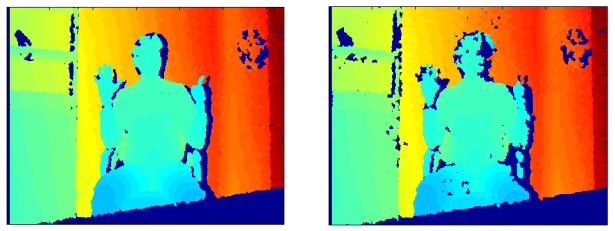
\includegraphics[width=0.5\textwidth]{images/twokin.png}
\caption{Difference between using a single Kinect and more than one Kinects}
\label{fig:twokin}
\end{figure}

On the other hand, multiple Kinects can result on better data quality for large objects or regions since each device can be responsible for capturing an specific part of an object or scene, resulting in more details for each component. Similar approach is implemented by the work at \cite{tong}, which aims to make a full three-dimensional scan of the human body by using three Kinects carefully positioned in order to avoid overlapping (and consequently, interference) between them as much as possible, as shown on Figure \ref{fig:3kin}.

\begin{figure}
\centering
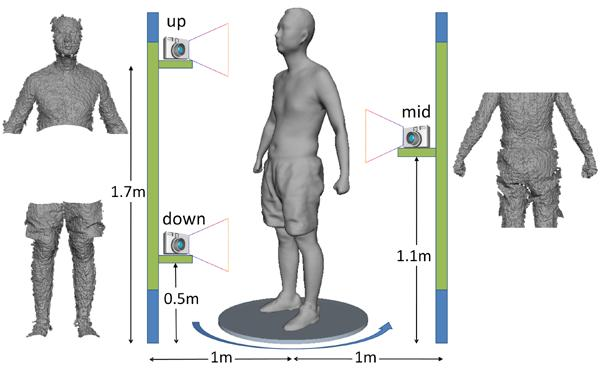
\includegraphics[width=0.5\textwidth]{images/3kin.jpg}
\caption{Three Kinect devices being used for a full scan of the human body with minimum overlapping \cite{tong}}
\label{fig:3kin}
\end{figure}

The main reason that made the authors decide for using multiple Kinects was because in order to capture a full human body, a single Kinect should be positioned around 3 meters away from the body, and the resolution would be very low, since little geometry information is captured on the depth map. Even using multiple frames to enhance the final resolution, the result wouldn't be acceptable.

Not only multiple Kinects, but multi-camera environments are used for three-dimensional reconstruction, since a single camera can just capture a two-dimensional projection of the scene. Not many works were found with regards to calibrating multiple Kinects. The most notable way of calibrating many RGB cameras in relation to a common reference is by processing images captured from a chessboard. The approach at \cite{matlab} became popular by providing a straightforward way to find chessboard corners and that's still largely used.

When multiple Kinects are present on a multi-camera configuration, the challenge is to develop methods that simultaneously calibrate the RGB sensor and depth sensors using a suitable calibration pattern. An approach to that is discussed on \cite{berger2011markerless}, which uses four Kinect devices for motion capture. This work investigates on reducing or mitigating the detrimental effects of multiple active light emitters, thereby allowing motion capture from all angles. The calibration approach used by the authors is to still use a chessboard pattern to calibrate the RGB and depth sensors simultaneously, but not a simple board printed on paper, instead they use a binary pattern consisting of diffuse and mirroring patches. The reflective patches act as mirrors and deflect the IR pattern to infinity while the diffuse patterns reflect the IR light and provide depth values in the captured image, which are finally used for calibration in the Matlab calibration toolbox \cite{matlab}. Many other studies for multiple Kinects are discussed on \cite{schroder2011multiple}.

Besides calibrating the depth and RGB maps simultaneously, for some cases it's also important to calibrate one Kinect in relation to the other and so be able to determine the relative position between them. On \cite{magnus2013}, among other works, it's used a calibration process introduced by \cite{herrera}, which not only explains the approach, but also releases a toolbox to perform the calibration, which is represented on Figure \ref{fig:herrera}.

\begin{figure}
\centering
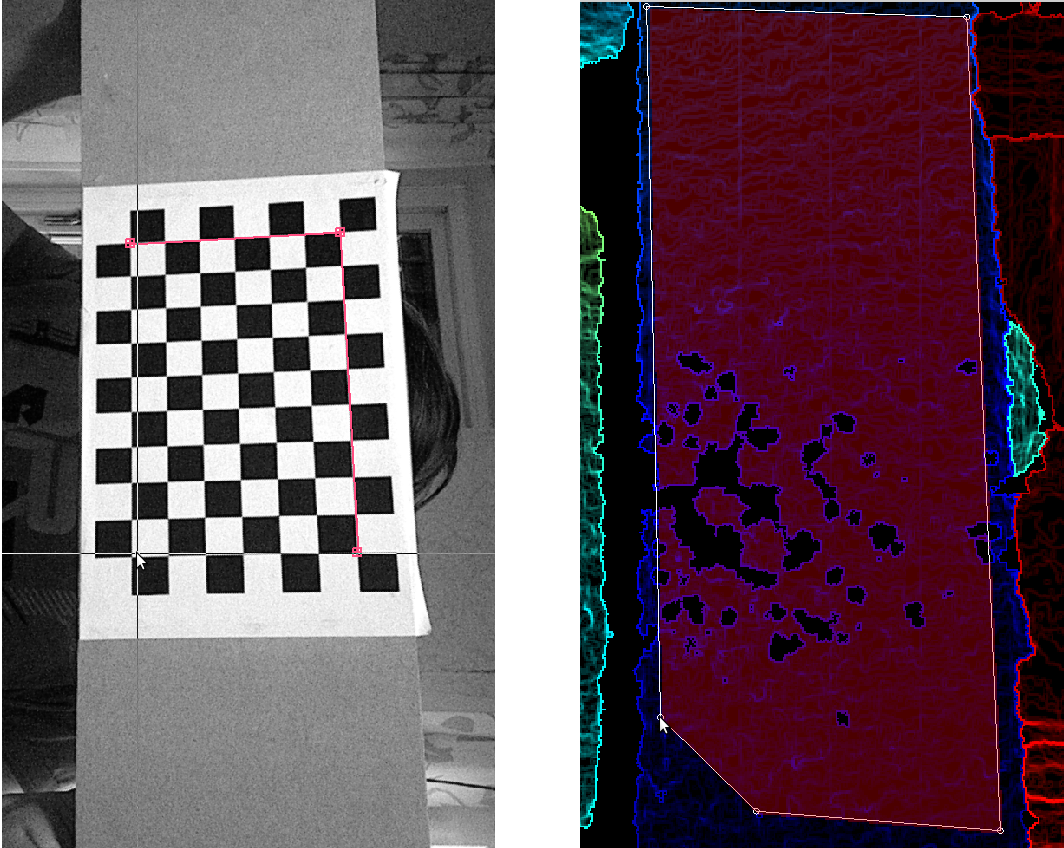
\includegraphics[width=0.5\textwidth]{images/herrera.png}
\caption{Calibrating Kinect using toolbox from \cite{herrera}}
\label{fig:herrera}
\end{figure}

That algorithm simultaneously calibrates the color camera and the depth camera, as well as the relative position between them. The color camera intrinsics is based on the following model: a 3D point is transformed into image coordinates and a disparity value from the disparity map at these coordinates is transformed into a 3D point.

\section{Hybrid-based tracking}

Since sensor-based methods rely solely on geometric information, sometimes it can fail for planar or smooth surfaces. On such cases, the results can be improved by combining geometric data with visual data. Different methods can be employed to detect specific features or objects in the scene, such as point detection, background modeling, image segmentation or classifiers based on supervised learning.

One approach to use visual information to improve geometric mapping is discussed on \cite{Hen10RGB}, which combines visual features with shape-based alignment. This paper introduces RGB-D mapping, a framework that can generate dense 3D maps of indoor environments despite the limited depth precision and field of view provided by RGB-D cameras. The core of this framework is a variant of the ICP algorithm, called RGBD-ICP, which uses the rich information contained in RGB-D data. First, the framework performs an initial estimate of the 3D camera transformation by applying RANSAC\footnote{Random sample consensus - an iterative method to estimate the parameters of a mathematical model} to SIFT\footnote{Scale invariant feature transform - an algorithm in computer vision to detect and describe local features in images} feature matches with depth values. The modified ICP algorithm combines these visual feature associations with dense point associations, and then the final transformations are used to create a pose graph, which at a final post-processing step is optimized in order to achieve a consistent map. Later on, the same authors released another paper \cite{Hen12RGB} where they avoid the expensive ICP step when enough features are identified on the image. Another work, at \cite{Engelhard11real-time3-d}, follows a similar approach but uses SURF \cite{bay} instead of SIFT features.

The closest to what is done on this work is the work by \cite{kinectkanade}, which improves the KinectFusion algorithm by using the Lucas-Kanade algorithm in cases of low geometric features.

An application of the hybrid-based tracking is also noticed on \cite{tryon}. It's a virtual try-on system that employs one Kinect sensor and one high definition camera. It covers the calibration of the HD camera in relation to the Kinect sensor, which is based on the OpenCV implementation of a standard chessboard calibration \cite{matlab}. On this work, the Kinect is used for skeleton tracking and height estimation, and the HD camera is used for capturing a better video from the user.

\xchapter{Solution architecture}{In this chapter I explain in details the steps performed in order to implement the objective of this work.}

In order to achieve the objectives of this work, it was necessary to implement some softwares and auxiliary codes, all of them based on other open source code or open source libraries. All the code implemented on this work was released under open licenses and is available on public repositories, which will be informed along this chapter. All the documentation about the code implemented on this work is available on the appendix.

\section{Environment}
\label{sec:env}

An augmented reality system is composed by two basic components: software and hardware. Hardware means input devices, displayed, processors and networks. Software means the augmented reality application plus trackers, image mergers, interaction functions and multi-modal interfaces \cite{tori2006fundamentos}. The implementation of the environment proposed by this work involved arrangement, configuration, implementation, calibration, transformation, communication and tunning.

The development environment chosen for the implementation is based on GNU/Linux, supported by the distributions Debian 6 (due to stability) and its variation Ubuntu 12.04 (the 12.04 was told to be more stable for many of the open libraries used by this implementation \cite{pcl14}). All the code was written in C/C++ and all used libraries are released under open licenses. Both machines employed on this environment are 32 bits, so there is no guarantee that it will work on 64 bits (but in theory it should). Since the relevant libraries have versions for both Windows and Linux systems, all code here is theoretically portable to Windows.

Two computers were employed on this environment, because, as it's going to be explained on next sections, the number of USB ports or throughput of one computer was not enough. The machine used for most of the tasks was a notebook Dell Inspiron 14R 5421-A20, Intel Core i7 with 8GB of RAM memory, 1 TB of disk space and 2 GB dedicated video card NVIDIA GeForce GT 640M LE. The other machine is a simple laptop, an ACER notebook with just 2 GB of RAM memory, an Atom processor dual-core and no dedicated video. The former runs Ubuntu 12.04 while the latter runs Debian 6. Most of the code implemented here is based on the KinectFusion (explained on section \ref{sec:kinfu}) implementation on PCL, which requires a Nvidia graphics card with CUDA support. There wasn't a native driver for that graphics card for Ubuntu, so it was necessary to use a third-party project called Bumblebee \cite{bumblebee}, which aims to provide support for Nvidia Optimus technology for GNU/Linux distributions. After compiling and installing its drivers, it was possible to run CUDA on Linux, by just prefixing an \textit{optirun} prefix before running any executable on the command line.

The multi-view environment proposed by this work is composed by two Kinects and one pair of augmented reality glasses.

The Kinects are from the first generation and most of its internal workings were explained on section \ref{sec:kinect}. For both, the depth sensor and RGB camera are used, but the audio features are not used for anything.

As explained on section \ref{sec:dirind}, an augmented reality experience can be classified in two different ways depending on how the user sees the mixed world. When the user sees the mixed world pointing his eyes directly to the real positions of the object or scene, this experience is classified as \textit{direct view}, while when the user sees the mixed world through a monitor screen or projector, this experience is classified as \textit{indirect view}. On this work, augmented reality glasses are used in order to guarantee a \textit{direct view} experience to the observer. The augmented reality glasses employed on this work are Vuzix Wrap 920AR, whose photo is on Figure \ref{fig:glasses}. This device has a VGA adapter that can be connected to the computer. It also has a motion tracker based on accelerometer and magnetometer which connects to a device's special port and allows softwares to track direction, viewing angle and motion of the user. Two modified USB cameras are placed on the front of the lenses (one camera on each lens) and be connected to the computer as two VGA webcams. Behind each lens, there is a screen whose resolution is 640 x 480 pixels. So, what the user sees in front of his eyes is a rectangular screen, which doesn't provide a full immersive experience. The glasses have three cables: a VGA (a single VGA output that provides access to both screens) and two USB (one for both cameras and the other that is an interface for the accelerometer/magnetometer data).

\begin{figure}
\centering
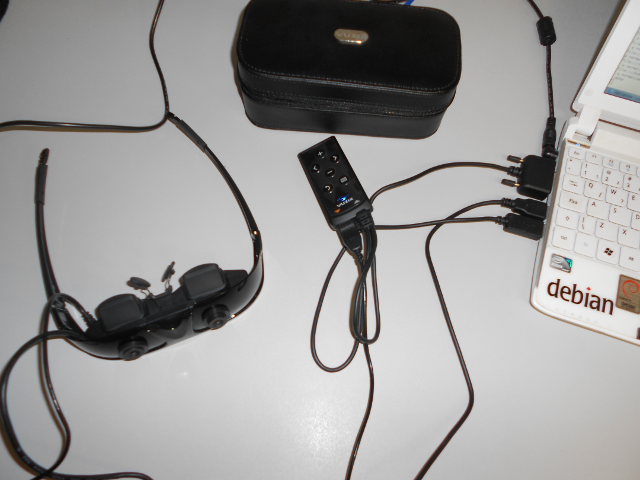
\includegraphics[width=0.5\textwidth]{images/vuzix.png}
\caption{Vuzix Wrap 920AR augmented reality glasses}
\label{fig:glasses}
\end{figure}

Back to the traditional augmented reality pipeline presented on Figure \ref{fig:arpipeline}, on Figure \ref{fig:pipeline} it's explained visually what is the pipeline for the augmented reality application implemented on this work.

\begin{figure}
\centering
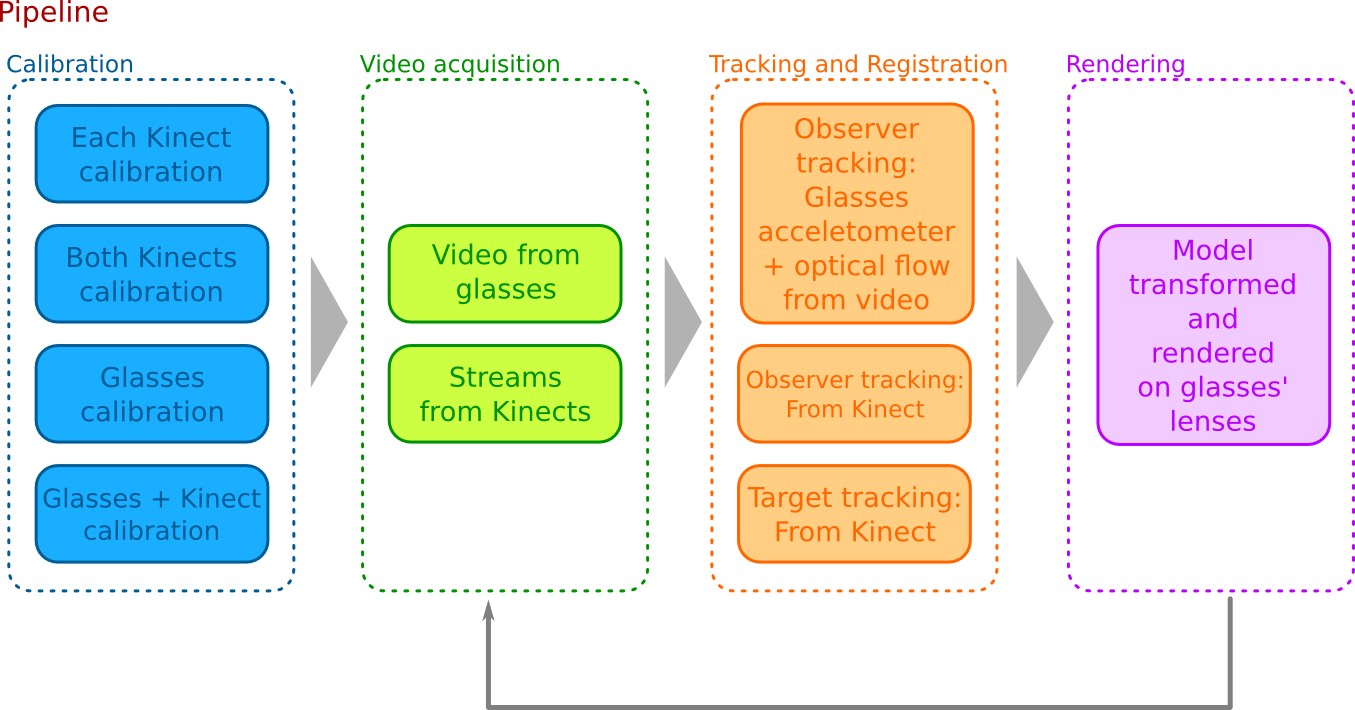
\includegraphics[width=1\textwidth]{images/pipeline.png}
\caption{Augmented reality pipeline}
\label{fig:pipeline}
\end{figure}

On the calibration stage, it's necessary to perform four different calibrations:

\begin{itemize}
  \item Calibrate each Kinect device separately;
  \item Calibrate one Kinect in relation to the other;
  \item Calibrate the augmented reality glasses;
  \item Calibrate the glasses in relation to the Kinect the captures the target model.
\end{itemize}

Each of these calibration processes will be covered in details on section \ref{sec:calibration}. On the video acquisition stage, the environment gets video streams and depth streams from both RGB cameras of each Kinect as well as the video stream from the glasses' lenses. On the tracking an registration stage, there are different approaches for tracking the observer (by just using the glasses or by using a second Kinect), while the target model is always tracked by a Kinect device. Information from the Kinects are registered as point clouds while information from the glasses are registered as transformation matrices. Finally, the target model, transformed to the observer's viewing point, is rendered along with some virtual image and displayed on the glasses' lenses. It is worth noticing that the merging of the real image with a virtual image is not on the scope of this work, which is focused on transformation, tracking and multi-view. More details on each of these stages will be provided along this chapter.

Back to the global view of the proposed environment represented on Figure \ref{fig:diagram} and idealized before the implementation of this environment, there is another diagram on Figure \ref{fig:env} that shows the actual implemented environment. It is worth noticing that the proposed environment was implemented as planned. The idea of this diagram is to make it easier to understand, from a higher level, how the proposed environment was actually implemented.

\begin{figure}
\centering
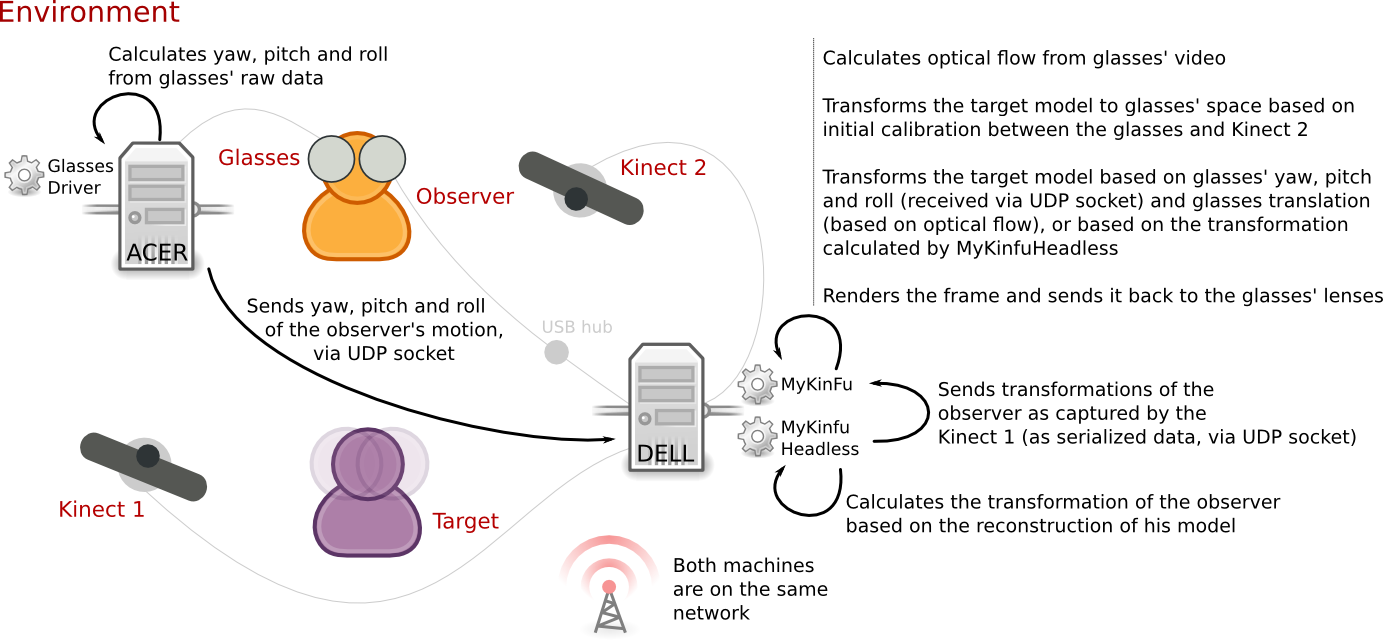
\includegraphics[width=1\textwidth]{images/env.png}
\caption{High level representation of the augmented reality environment implementation}
\label{fig:env}
\end{figure}

The diagram at Figure \ref{fig:env} represents the main components of the augmented reality environment and their main roles. First of all, it's worth noticing that all these components and roles will be explained in more details on sections \ref{sec:method1} and \ref{sec:method2}. As it will be better explained on section \ref{sec:kinectscalib}, each Kinect needs to be connect to not only a USB port, but more than that, a USB hub. This is also stated on \cite{kinecthacks} on the section about \textit{Multiple Kinects}. Most computers have two USB hubs, which allows the user to use at most two Kinects at the same time, and this is the case here too. The Dell computer employed here has three USB ports, where two are on the same hub. Since each Kinect gets a USB port from each hub, the remaining USB port is used by the video input cable from the glasses and the VGA output cable from the glasses are connected to the Dell computer too. This way, it's possible to avoid transferring video streams (regardless input or output) over the network, what could add a reasonable delay to the whole process. The remaining connector from the glasses is the USB cable responsible for streaming the accelerometer/magnetometer data. This one is connect to the Acer computer, since its computation is not costly and transferring a tuple of values over the network is not costly either. Both computers are on the same network (more details about this on section \ref{sec:comm}. The Dell computer is responsible for running the heaviest softwares, which are two: MyKinFu (based on PCL's KinectFusion implementation), which is the core of this environment and connects all other components, and MyKinFuHeadless, which is based on the former but just keeps the code necessary to calculate the transformation of the movement performed by the observer.

To finish this section, Figure \ref{fig:expenv} is a photo of the experimental environment arranged for this implementation.

\begin{figure}
\centering
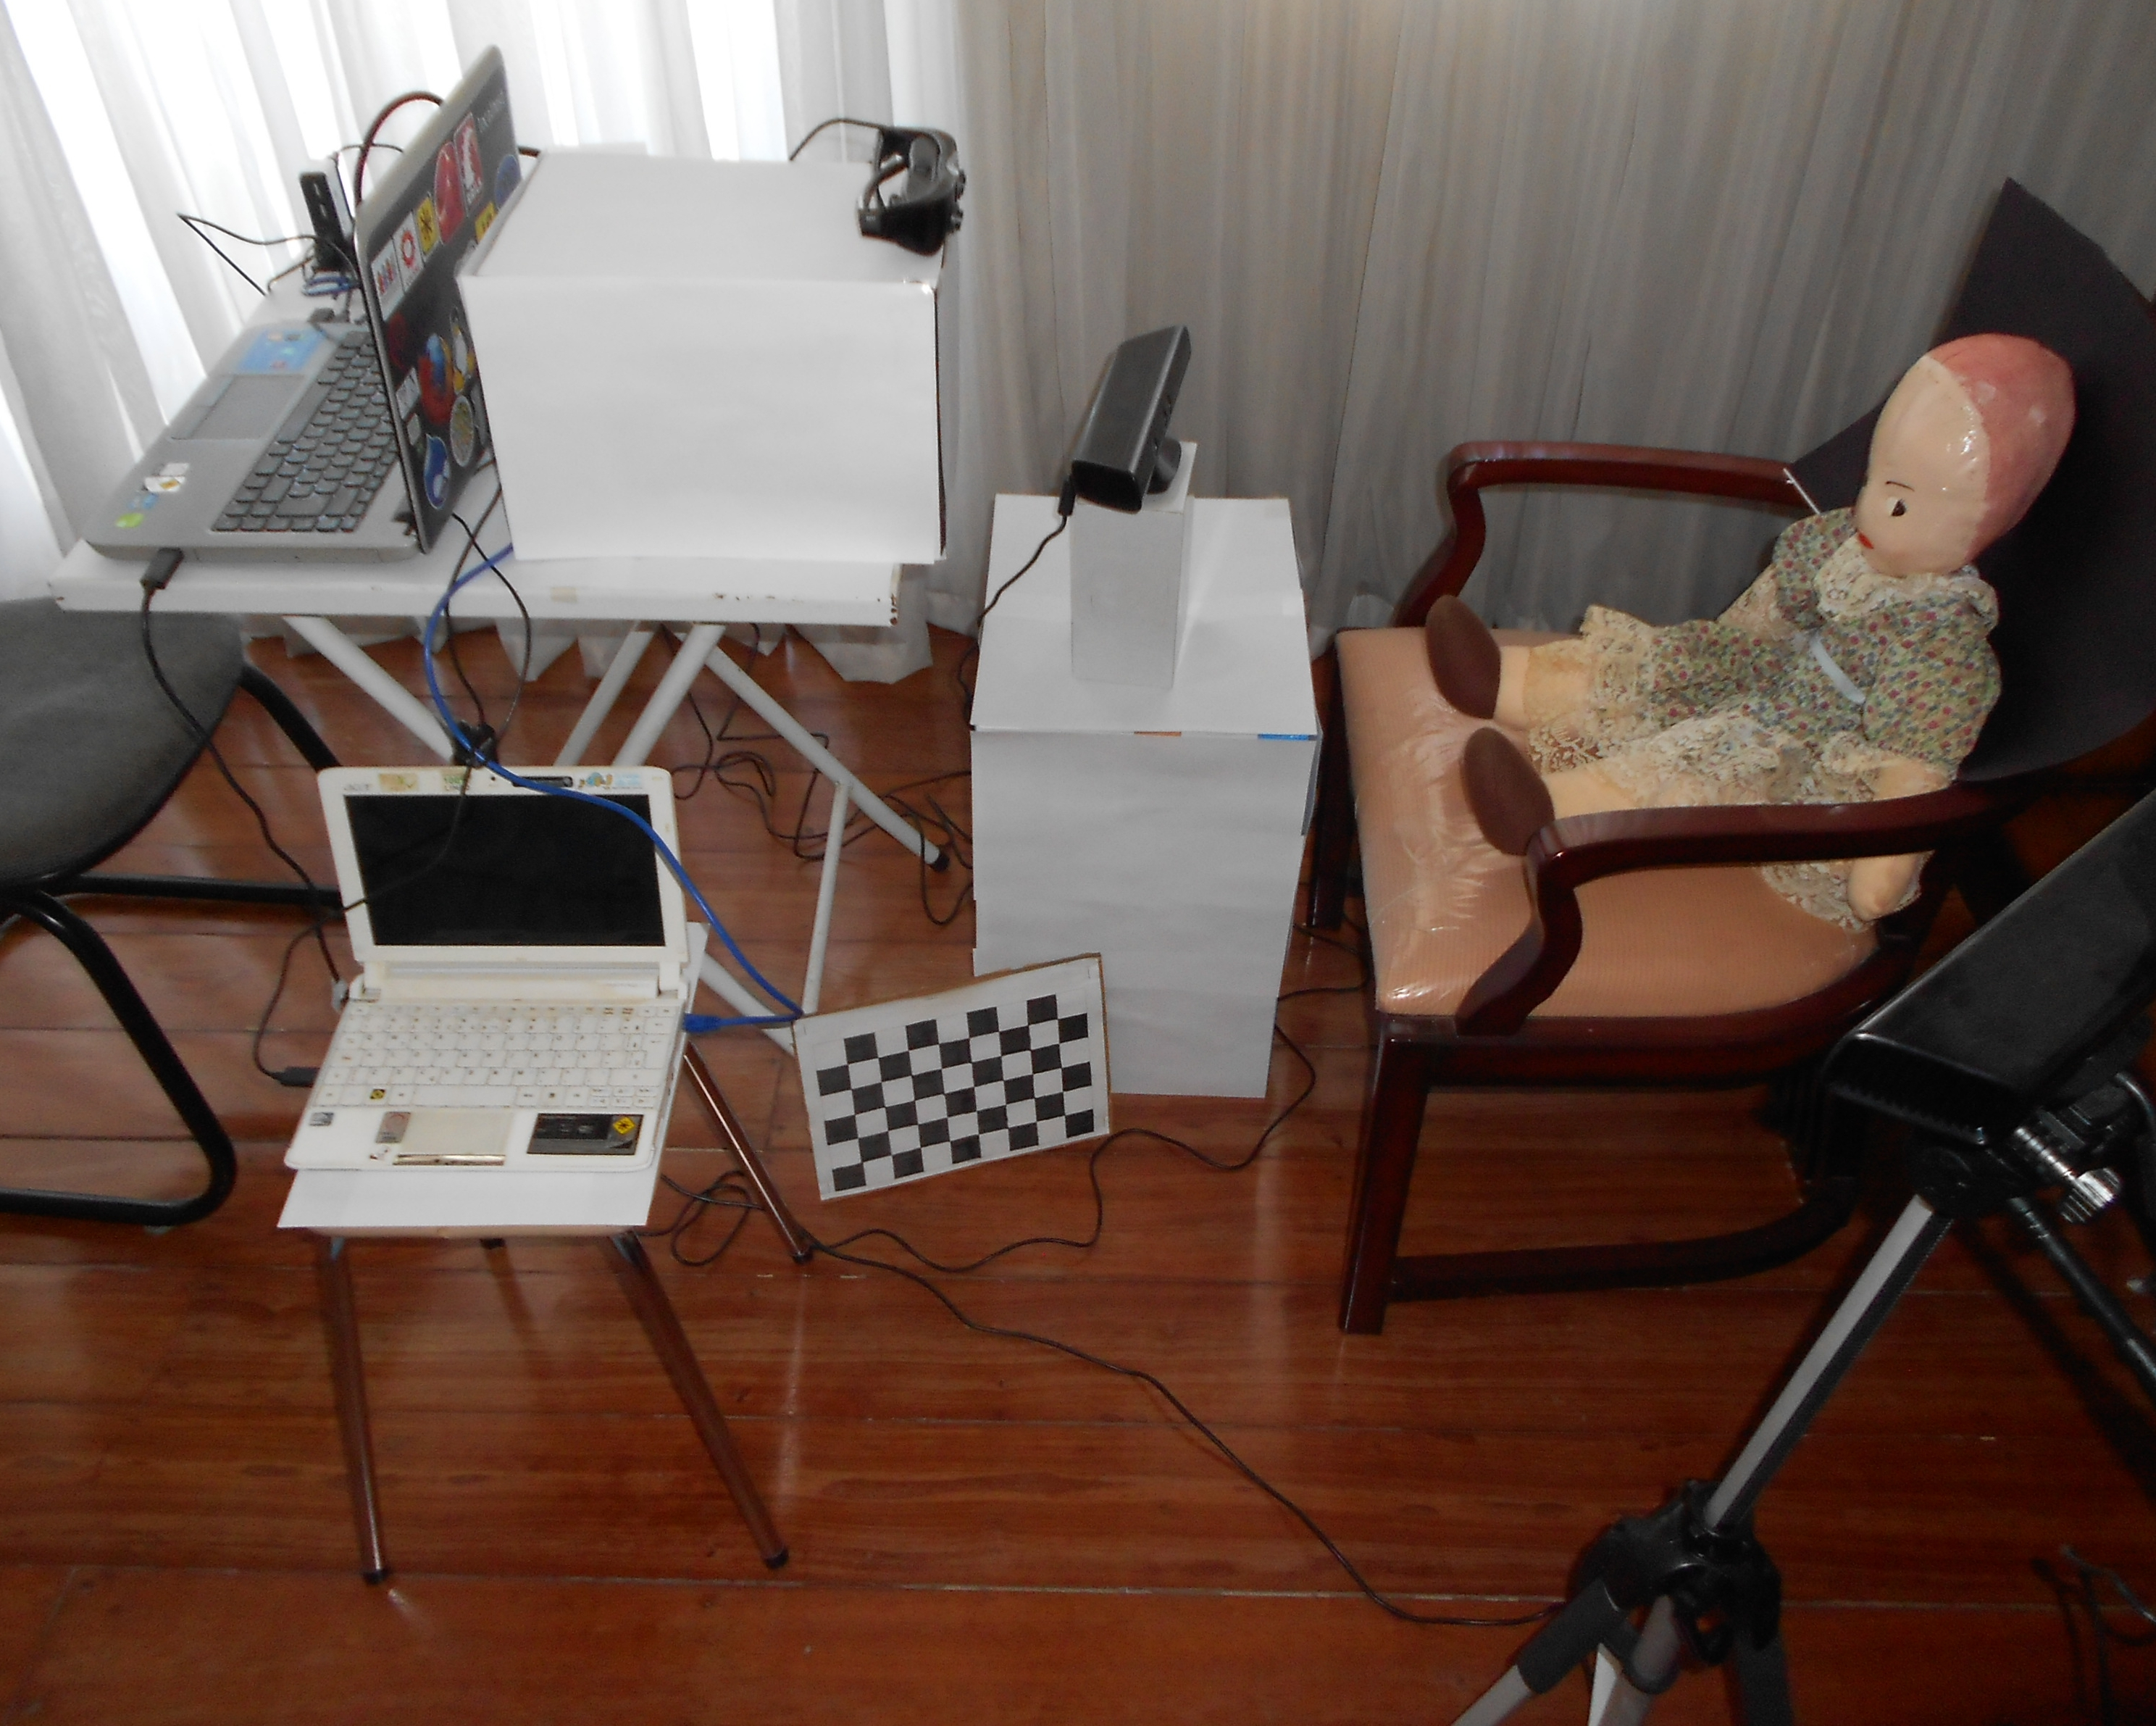
\includegraphics[width=0.7\textwidth]{images/expenv.jpg}
\caption{Experimental environment arranged for the implementation}
\label{fig:expenv}
\end{figure}

Since it would be hard to find two volunteers to act as observer and target model during this implementation, on the experimental environment a movable square box with the augmented glasses over it is used as observer while a doll is employed as the target model. In order to be able to easily segment the target model's head, a black background is placed behind it and removed by color matching. As explained on section \ref{sec:kinfu}, better results are achieved for surfaces with enough irregularities or details, so there was a concern that using a spheric head for the target model and a square head for the observer wouldn't give the best results, thus real persons were employed on the calibration stage and on the environment evaluation, which will be presented on section \ref{sec:results}.

\begin{figure}
\centering
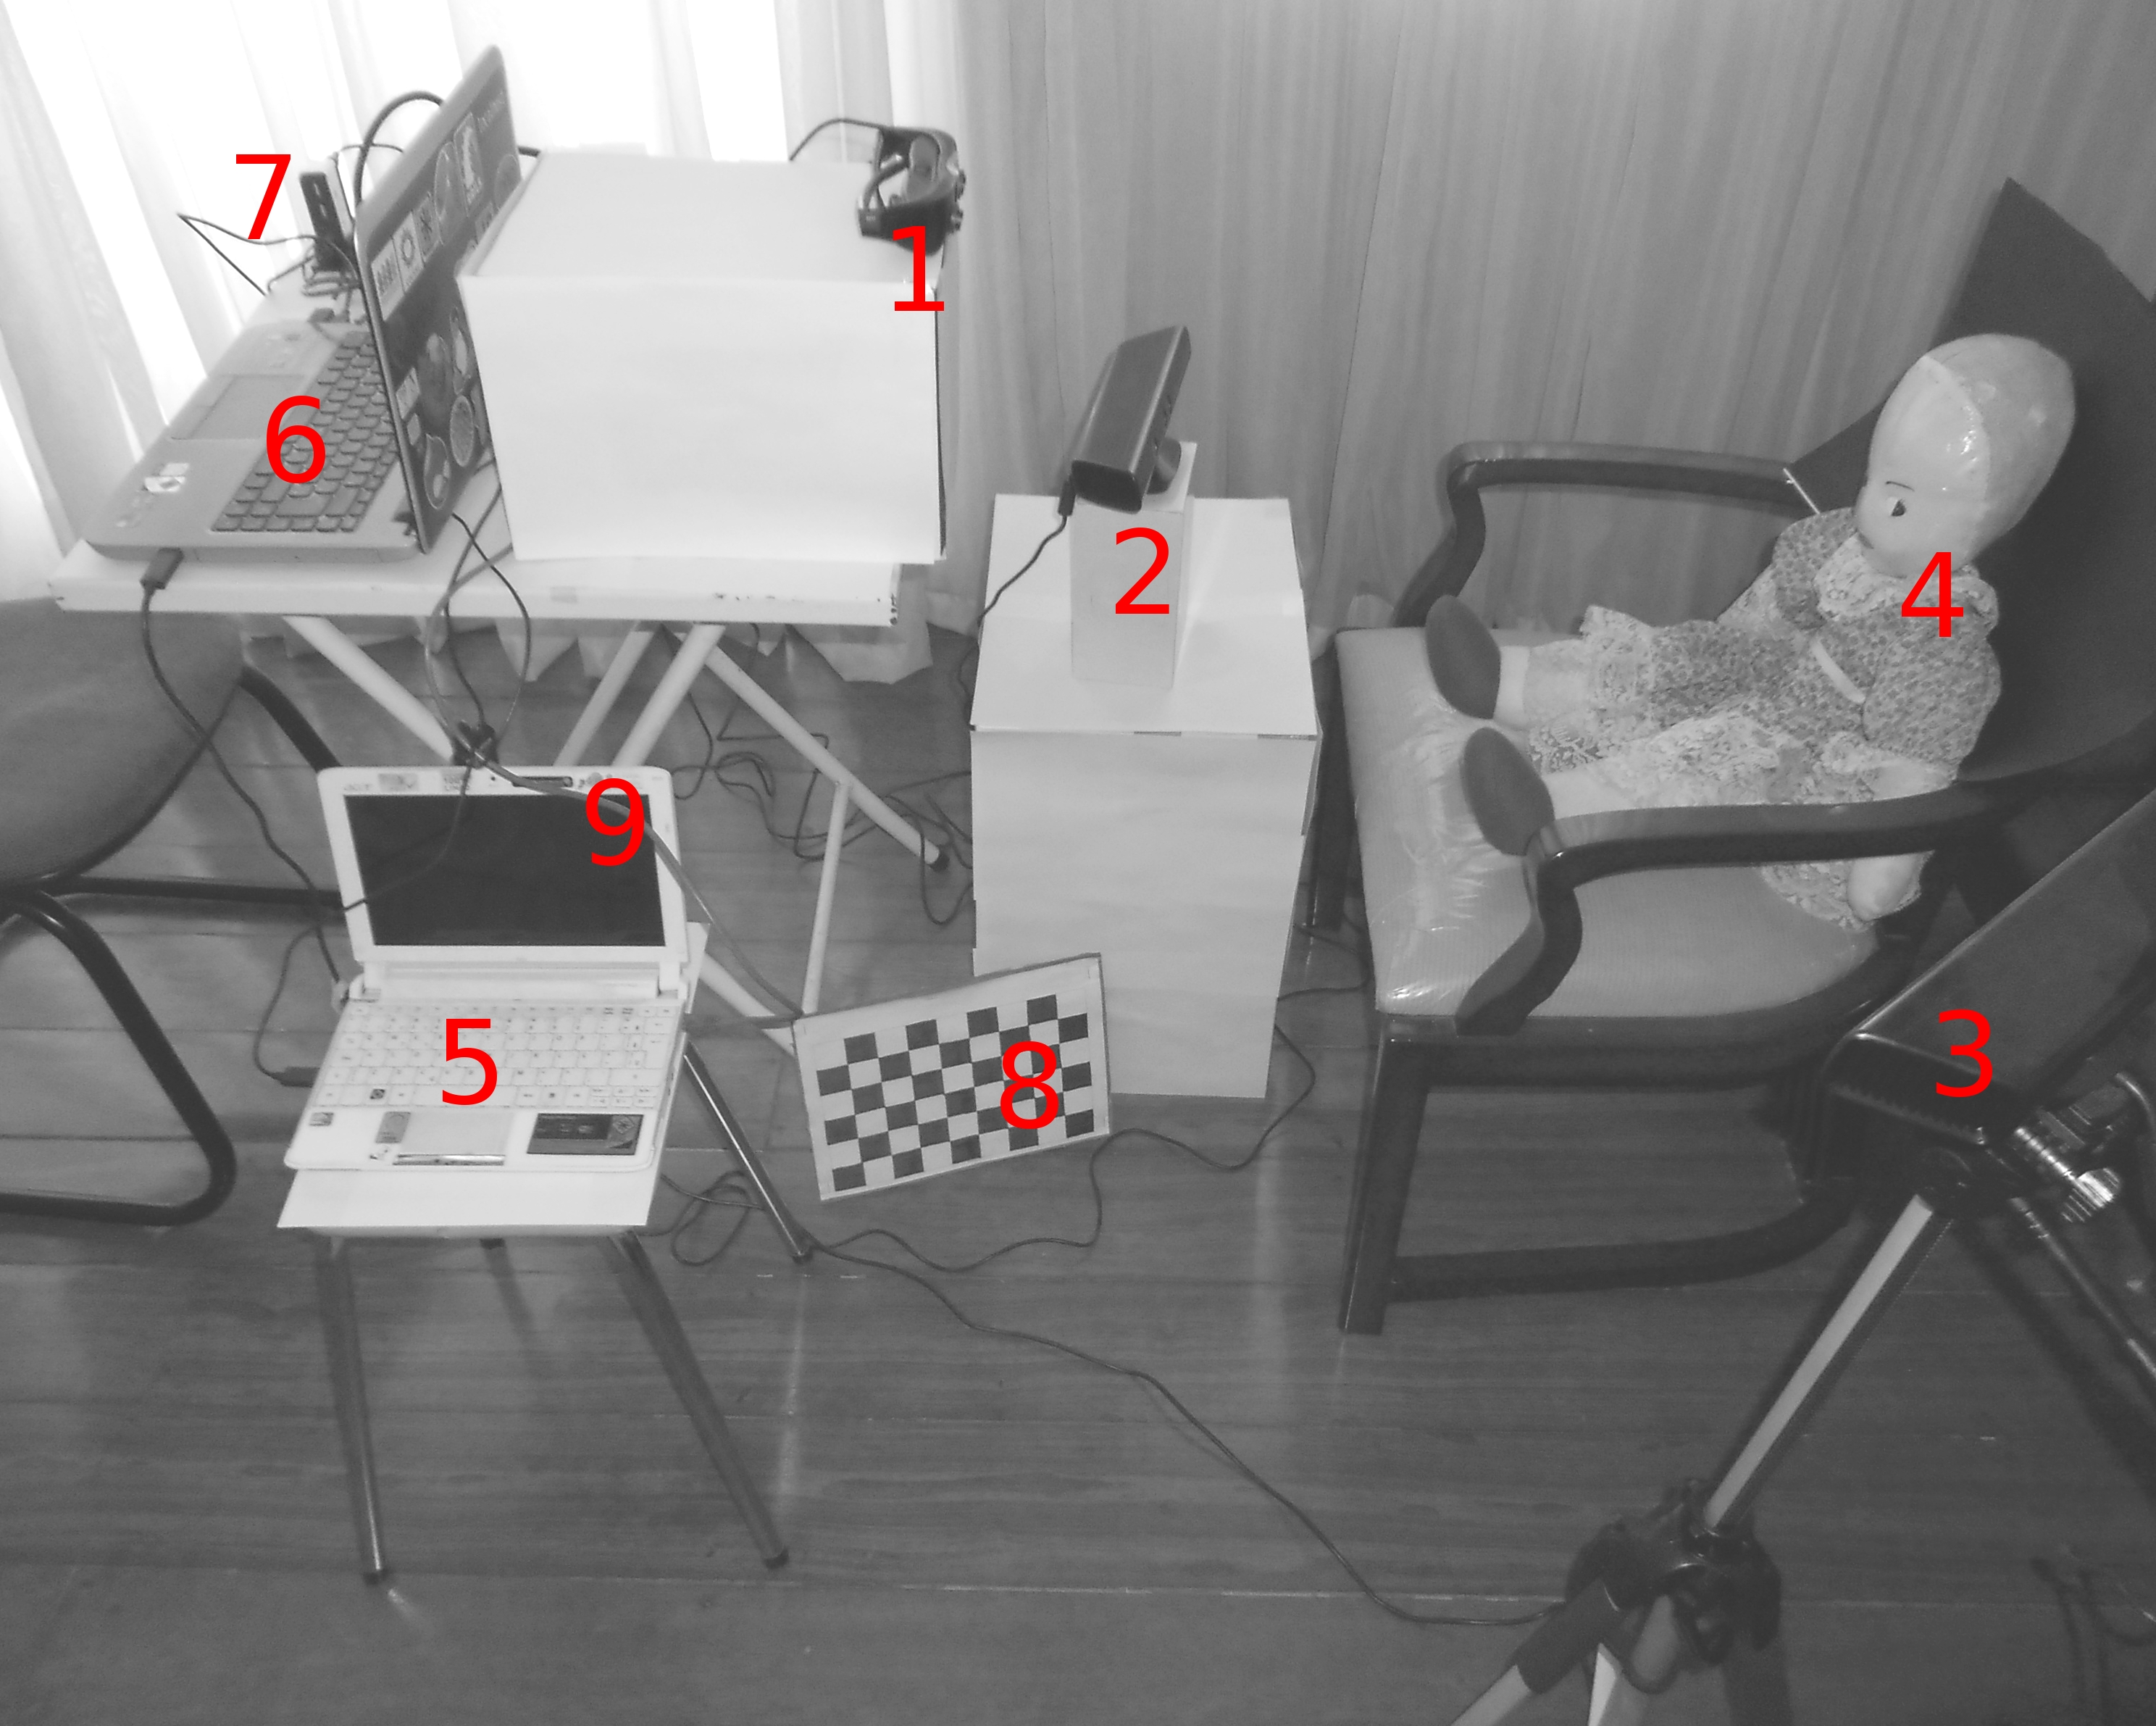
\includegraphics[width=0.7\textwidth]{images/expenv2.jpg}
\caption{Experimental environment arranged for the implementation with each component identified by a number}
\label{fig:expenv2}
\end{figure}

On Figure \ref{fig:expenv2} each component is numbered for easy identification. They are:

\begin{enumerate}
  \item Augmented reality glasses over a movable box, which acts as the observer;
  \item Kinect that captures the target model;
  \item Kinect over a tripod, to capture the observer;
  \item A doll that acts as the target model;
  \item The Acer computer, employed just to calculate the observer's movement based on accelerometer/magnetometer data from the glasses;
  \item The Dell computer, responsible for the core code and the main computation;
  \item An external USB hub with external power supply, needed by the video USB cable of the glasses (since the Kinect uses most of the power of the hub which it is connected to)
  \item The chessboard used for calibration;
  \item Network cable that connects both computers.
\end{enumerate}

There was a concern about the amount of sunlight arriving at the room where the environment was built, because, as stated on section \ref{sec:kinect}, the sunlight's wide band IR has enough power on Kinect's IR sensor range in order to blind it. Another concern was regarding the distances between each component, which were all below one meter, as shown on Figure \ref{fig:expenv3}.

\begin{figure}
\centering
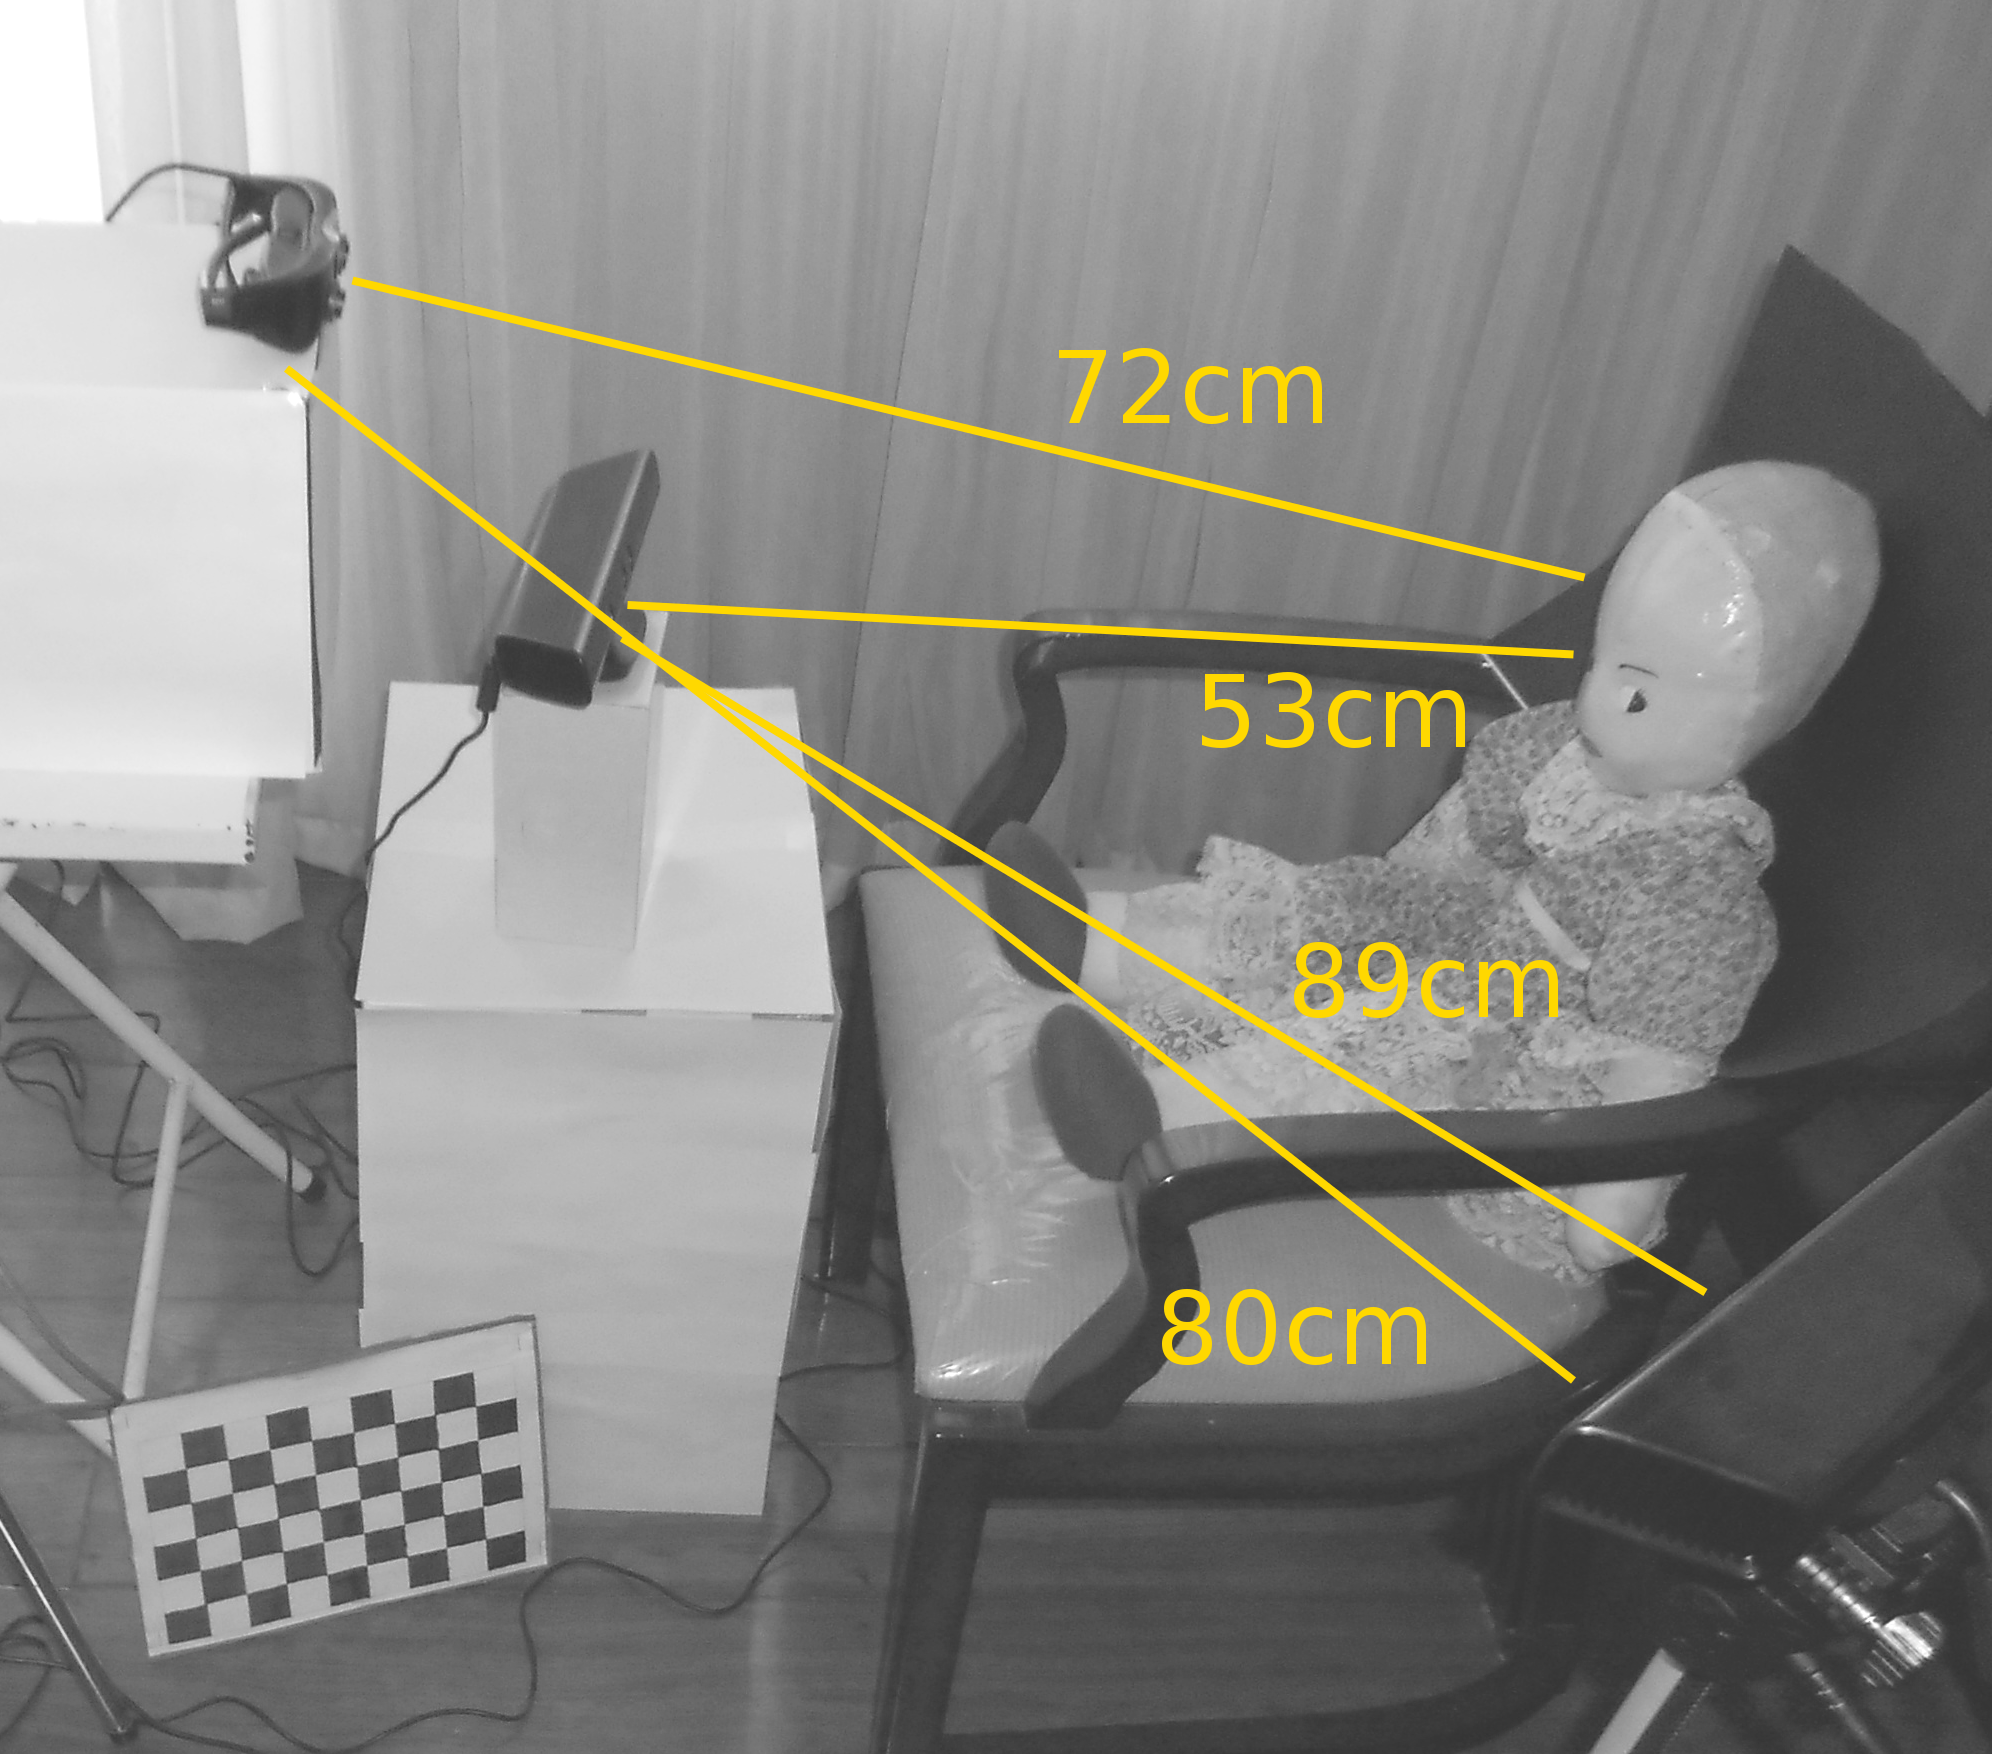
\includegraphics[width=0.7\textwidth]{images/expenv3.png}
\caption{Distances between each component on the experimental environment}
\label{fig:expenv3}
\end{figure}

Once the environment is ready, the next step is the calibration, which will covered on the following section \ref{sec:calibration}.

\section{Calibration}
\label{sec:calibration}

This section will cover the calibration of each component of the multi-view environment (each Kinect and the augmented reality glasses), as well as the calibration between both Kinects and the calibration between the glasses and one Kinect.

\subsection{Augmented reality glasses calibration}
\label{sec:glasses}

As informed on the manufacturer's support website \cite{vuzixsupport}, the API the accompanies the device doesn't have support under GNU/Linux environments. Under Microsoft Windows or Macintosh environments, calibration could be done by using a software provided by the manufacturer. Since one of the objectives was that the environment worked fully on a GNU/Linux environment, it was decided to implement an open driver for Linux that could be able to get raw data from the accelerometer/magnetometer and convert those to yaw, pitch and roll according to the movement of the observer's head, as shown on Figures \ref{fig:glasses1} and \ref{fig:glasses2}. The development of this driver was guided by the information on the Vuzix SDK guide \cite{vuzixsdk}.

\begin{figure}
\centering
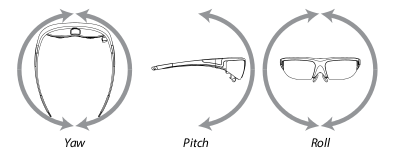
\includegraphics[width=0.7\textwidth]{images/glasses1.png}
\caption{Capturable movements from glasses \cite{vuzixsdk}}
\label{fig:glasses1}
\end{figure}

\begin{figure}
\centering
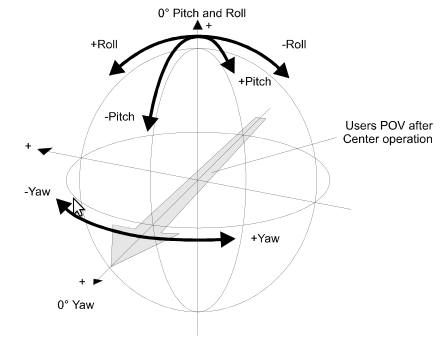
\includegraphics[width=0.7\textwidth]{images/glasses2.png}
\caption{Coordinates system of augmented reality glasses' tracker \cite{vuzixsdk}}
\label{fig:glasses2}
\end{figure}

The coordinates system of the augmented reality glasses' tracker is represented on Figure \ref{fig:glasses2}. The zero point of yaw movement is looking straight ahead. On the Wrap 920AR model, yaw and roll are valid over the range of -180\degree to +180\degree, while valid values for pitch are over the range of -90\degree to +90\degree. The zero point is forward for all axes. Yaw increments to the left, roll increments as the head turns towards the right shoulder and pitch increments as the user looks up.

The implemented driver has two major components: a \textit{rules} file, that allows its correct recognition by the computer, and a \textit{decoder}, written on C/C++, responsible for analyzing the raw data that comes from the glasses. The driver recognizes the device connected on the USB port and maps it to the location \textit{/dev/wrap920AR}, as virtual device. In order to that, a rules file is placed at \textit{/etc/udev/rules.d}, that contains the device identification (defined by properties \textit{VendorID} and \textit{ProductID}) and the path to the executable file that needs to be run when such device is recognized. This executable is the \textit{decoder}, a C++ program that, based on device's input data, returns values for yaw, pitch and roll. Those values are returned as Euler angles, as integer values in order to reduce little variations caused by interference and thus provide more stability. The rules evaluation and mapping to the correct location is done by \textit{udev}, an utility to manage paths under \textit{/dev} on UNIX-based systems, through evaluating rules defined by the system's administrator \cite{udev}. Evaluation is done when the device is plugged to the computer. In the case here, it was also necessary to blacklist some drivers at kernel level in order to avoid misinterpretation of the glasses by the computer.

The decoder receives raw data from the glasses, which are organized as blocks of 42 bytes structured like Table \ref{tab:glassesdata}.

\begin{table}
\caption{Raw data provided by the glasses' tracker}
\label{tab:glassesdata}
\centering
\begin{tabular}{|c|c|c|}
\hline
Magnetometer X                & Magnetometer Y                & Magnetometer Z\\
\hline
Accelerometer X                & Accelerometer Y                & Accelerometer Z\\
\hline
Low bandwidth & Low bandwidth & Low bandwidth \\
gyro X & gyro Y & gyro Z \\
\hline
High bandwidth & High bandwidth & High bandwidth \\
gyro X & gyro Y & gyro Z \\
\hline
\end{tabular}
\end{table}

There are four tuples, related to coordinates $x$, $y$ and $z$ from the accelerometer, magnetometer and low bandwidth and high bandwidth gyros (a tuple for each sensor). Values are over the range from -32768 to +32768.

The code of the decoder was based on the one at \cite{vuzixdriver}, a prototype of a Linux driver for another model of the Vuzix augmented reality glasses, the Vuzix Wrap 920VR. The version implemented on this work is openly available at \cite{masterproject}.

The device calibration is done on the first run (or if any calibration file is found) and is based on the averages for the maximum and minimum values retrieved for each sensor. Assuming that the driver is correctly installed on the computer, the steps in order to calibrate it are the following:

\begin{enumerate}
  \item Connect the glasses to the USB port
  \item Put the glasses over a flat surface and with little magnetic interference (for example, far from cell phones)
  \item Check the glasses log (as shown on Figure \ref{fig:glasseslog}) and move the glasses around and on all possible directions until the values on the screen don't change
\end{enumerate}

\begin{figure}
\centering
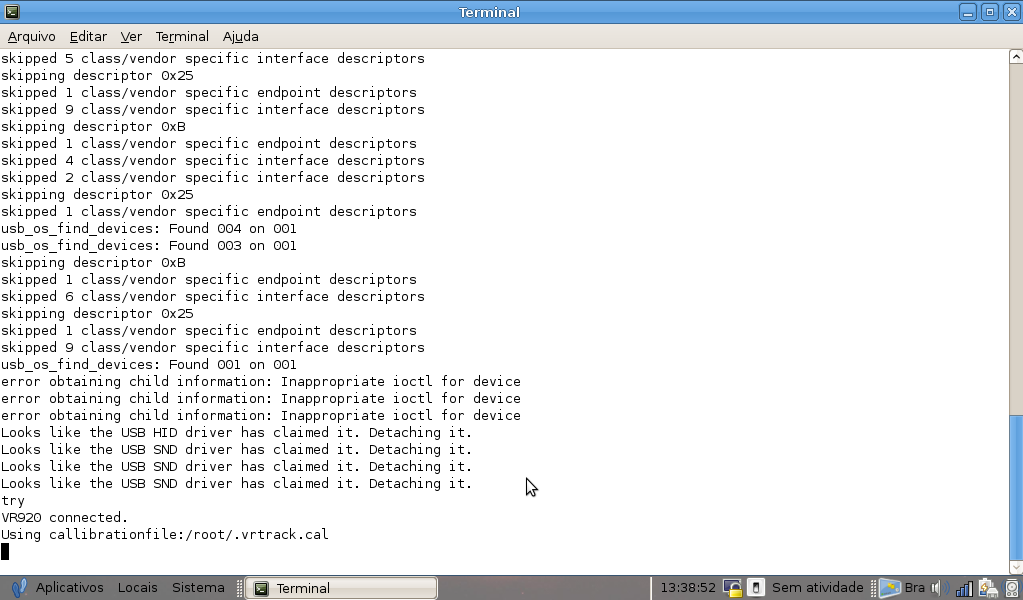
\includegraphics[width=0.7\textwidth]{images/glasseslog.png}
\caption{Glasses calibration log}
\label{fig:glasseslog}
\end{figure}

The calibration result is is stored on a configuration file on the user's home directory. Those values will be used on the next run of the tracker. If the glasses are going to be used on another environment different from the one where it was calibrated, a new calibration might be necessary. In order to do that, it's enough to remove the calibration file created on the user's home directory.

The calculated results for yaw, pitch and roll are available at the location \textit{/dev/wrap920AR} and can be read by any program by simply using a file handler, since on UNIX-like systems, the locations under \textit{/dev} are like normal files. An example was an auxiliary code that was implemented in order to test the glasses' tracker accuracy, and also publicly available at \cite{masterproject}. It reads glasses' tracker data and moves a three-dimensional cube accordingly, as shown on Figure \ref{fig:glassescube}. A video is available at \cite{videos}.

\begin{figure}
\centering
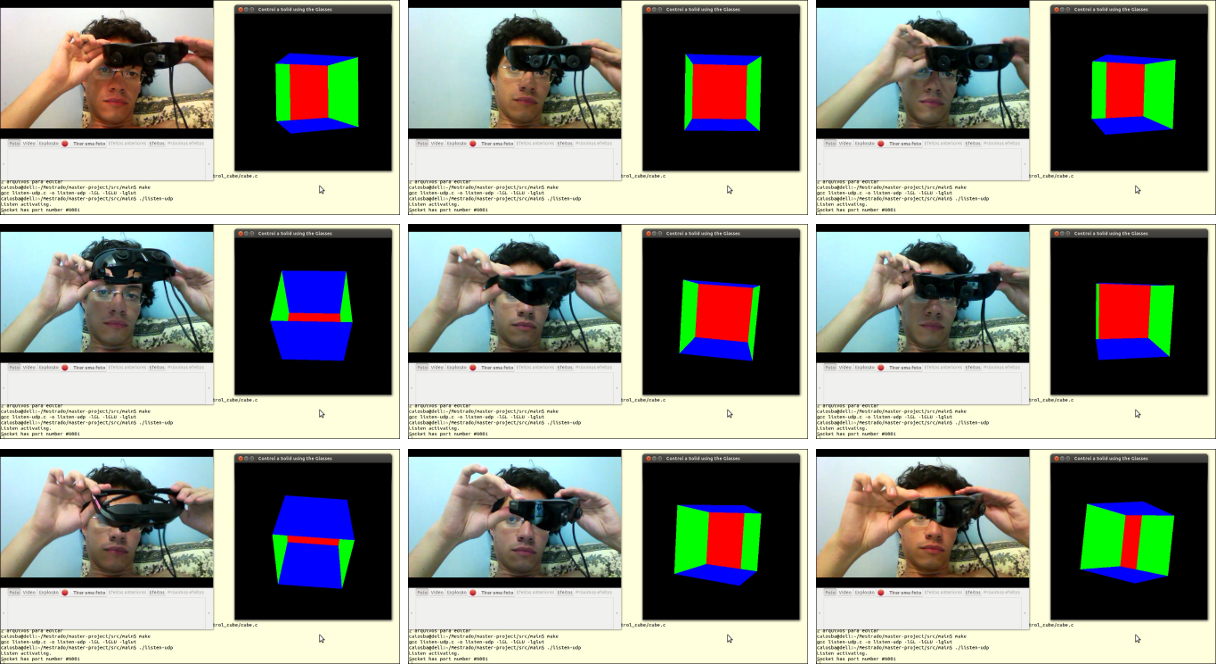
\includegraphics[width=0.7\textwidth]{images/glassescube.png}
\caption{Glasses' tracker controlling a virtual cube in order to check its accuracy}
\label{fig:glassescube}
\end{figure}

Glasses' tracker information is used as one of the approaches for tracking the observer's head, as will be explained on section \ref{sec:method1}.

\subsection{Initial calibration between Kinects}
\label{sec:kinectscalib}

Two Kinect devices are used to capture the observer and the target object. Kinect already had drivers for Linux, implemented within the project OpenKinect \cite{openkinect}. After the initial calibration between two Kinects, it's possible to know the relative position between them, by putting a central object that can be captured by both devices.

But first, it's necessary to calibrate the maps of each Kinect. As explained on section \ref{sec:kinect}, the Kinect provides two streams: color stream (as an RGB map) and depth stream (as a depth map). The depth map obtained at this stage is not yet ready for immediate usage, because there is no correspondence between the pixels of the depth map and the pixels of the RGB map. The intuition is that for each pixel on the RGB map, there is a correspondent pixel on the depth map. Figure \ref{fig:kinectnotcal} shows the images from depth map and RGB map where no calibration was done relative to the correspondences between pixels of both maps.

\begin{figure}
\centering
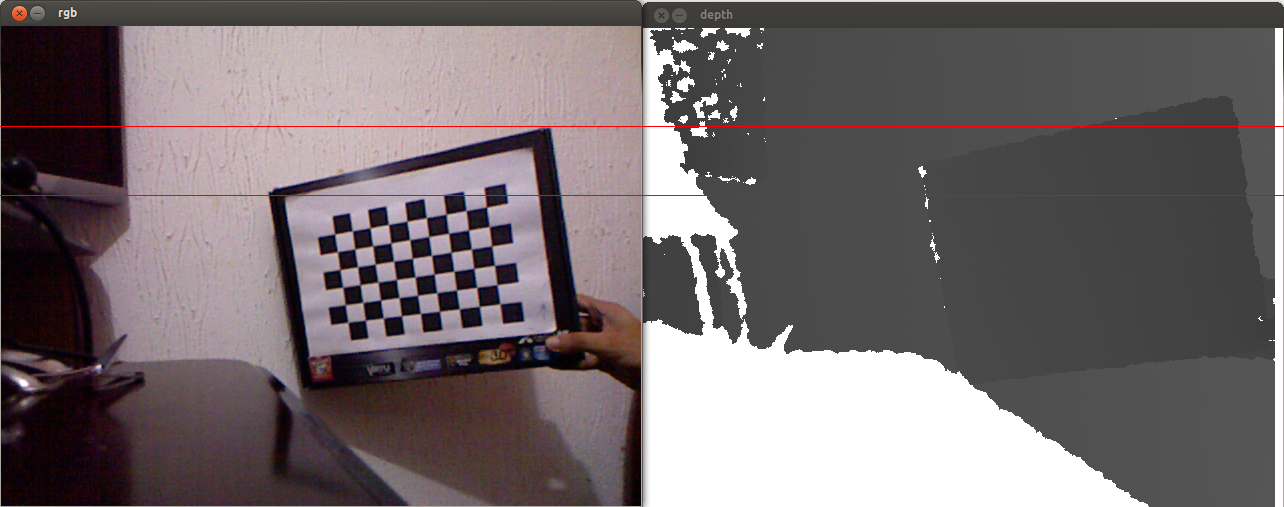
\includegraphics[width=0.7\textwidth]{images/kinectnocal.png}
\caption{RGB map and depth map with no matching between them}
\label{fig:kinectnotcal}
\end{figure}

When looking for alternatives for this calibration, it was found that OpenNI \cite{openni} could be a good solution for this calibration, through the \textit{libfreenect} driver. OpenNI is a framework that provides many features for development of middlewares and applications for three-dimensional sensing. OpenNI provides a functionality to automatically calibrate the RGB and depth sensors, by using data stored on Kinect's firmware. This calibration, called \textit{depth registration}, is enough for most of the applications, but better precision could be achieved by employing more specialized methods. It was decided to use the algorithm from \cite{burruscal} explained on section \ref{sec:kinect}, largely used by many applications (\cite{herrera}, for example). The program implemented for this calibration is written in C and uses the OpenCV \cite{opencv} library. Code can be found at \cite{masterproject}. The result of this calibration can be checked on Figure \ref{fig:kinectcal}.

\begin{figure}
\centering
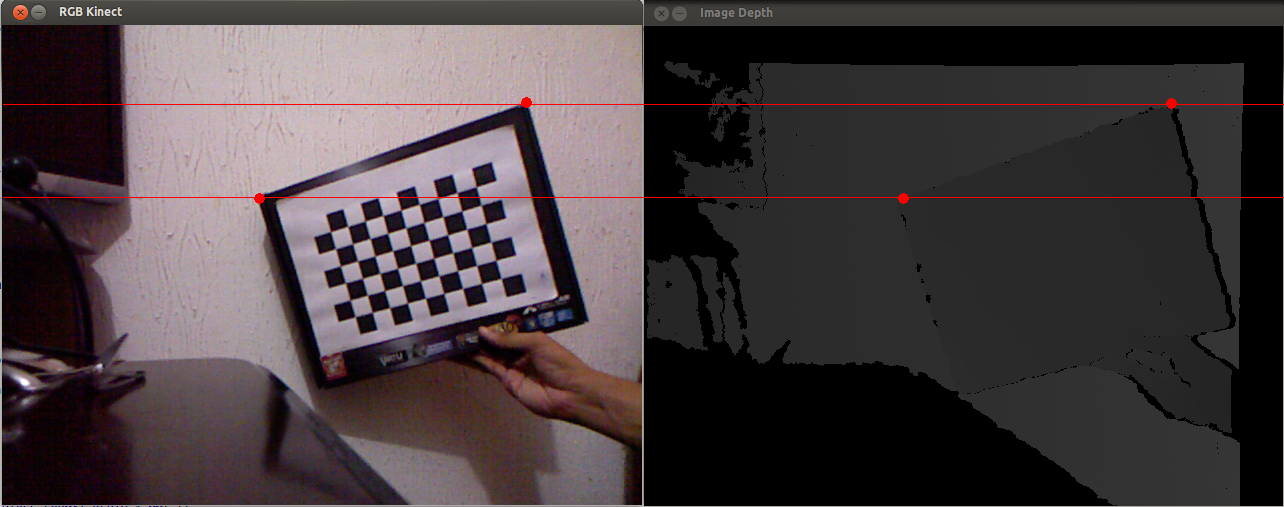
\includegraphics[width=0.7\textwidth]{images/kinectcal.png}
\caption{RGB map and depth map with depth registration enabled}
\label{fig:kinectcal}
\end{figure}

As addressed on section \ref{sec:kinect}, when multiple Kinects illuminate the same area with their IR projectors, interference is created. The random pattern that each Kinect produces from its diffraction grating is burned into the hardware. Extra dots added means that noise is added to the pattern too, and it confuses the depth differencing algorithm. This results in bad values randomly scatters on the depth window \cite{kinecthacks}. The approach here to avoid the interference between the Kinects is to calibrate them separately, but using a fixed calibration object on the center between them. The calibration object is a chessboard printed on both sides of a piece of carton.

Once the Kinects are calibrated and the intrinsic parameters are known, it's possible to know their positions given a chessboard pattern. These are the extrinsic parameters and are composed by a rotation matrix and a translation vector, that, when combined, take the points from the chessboard's coordinates system to the camera's coordinates system. Once the extrinsic parameters are known and the position of the chessboard in relation to camera is also known (this position is known initially), it's possible to define that the chessboard is the origin of this coordinates system and thus transform the cameras to this system.

The translation and rotation of an object in relation to the camera is equivalent to the transformation of the object to the camera's space, given by:

\begin{center}
$v' = R \times v + t$
\end{center}

Since the inverse of the rotation matrix is simply its transpose, it's possible to get the transformation of the camera on chessboard's space:

\begin{center}
$R^{-1} = R^{T}$
\end{center}

\begin{center}
$v = R^T \times v' - R^T \times t$
\end{center}

Finally it's possible to obtain the homogeneous transformation matrix (4x4):

\begin{center}
$M = \begin{matrix}
    R^T & -R^T \times t \\
    0 & 1 \\
    \end{matrix}$
\end{center}

\begin{figure}
\centering
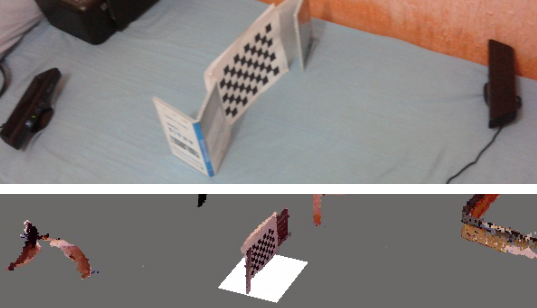
\includegraphics[width=0.5\textwidth]{images/panda.png}
\caption{Two Kinects in action: above, the real configuration (two Kinects capturing the same object) and below, the virtual image combined}
\label{fig:panda}
\end{figure}

Since the reference point is the same for both, the position of a Kinect in relation to the other can be estimated. Figure \ref{fig:panda} shows a reconstructed chessboard captured by two Kinects in order to validate this calibration. This code is also available at \cite{masterproject}. At this step, the system has the pose of each Kinect, and so it's ready to capture the observer and the target model.

\subsection{Initial calibration between Kinect and glasses}
\label{sec:kinect2glasses}

The final step for the calibration stage is the calibration between the Kinect and the glasses, this way, it's possible to make a first transformation of the model from the Kinect's point of view to the observer's point of view, and for tracking and later transformations, the system will use data from the glasses' tracker or from the Kinect that captures the observer.

The implementation for this stage was based on OpenCV \cite{opencv} and the library \textit{libfreenect} \cite{openkinect}. The code for this calibration was implemented on C++ and is available at \cite{masterproject}. When this code runs, it first calibrates each camera (glasses and Kinect) and then does the stereo calibration between them. The results (rotation matrix and translation vector) are stored on a file that is used as input by the main application. The approach employed here is similar to the one mentioned on \cite{tryon}, which is a virtual fitting room powered by a Kinect device and a high definition camera. The calibration on that work is based on OpenCV through capturing 30 chessboard poses.

Here, first, the Kinect device is accessed by the \textit{freenect} driver and a new thread is started, which is responsible for capturing a certain number of chessboard patterns by both cameras. This number was configured as 40 patterns; the board has 8 horizontal squares and 5 vertical squares, and each square has dimension 3cm x 3cm. This information is important for the calibration process.

Each frame of each video source is converted to grayscale and OpenCV's \textit{findChessboardCorners} function is used to check for a chessboard pattern on that frame. Here it's used adaptive thresholding to convert the image to black and white, rather than a fixed threshold level (computed from the average image brightness). This function will return a non-zero value if all the corners are found (that's why it's necessary to inform them previously) and if they are in order. If both input frames are views of the chessboard pattern, the function \textit{cornerSubPix} is called in order to achieve more accurate coordinates of the identified squares, since the coordinates determined by \textit{findChessboardCorners} are just approximations. The \textit{cornerSubPix} function iterates to find the sub-pixel accurate location of corners, as shown on Figure \ref{fig:cornersubpix}.

\begin{figure}
\centering
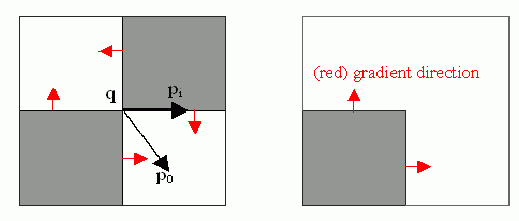
\includegraphics[width=0.5\textwidth]{images/cornersubpix.png}
\caption{How OpenCV's cornerSubPix function works \cite{opencvfd}}
\label{fig:cornersubpix}
\end{figure}

Sub-pixel accurate corner locator is based on the observation that every vector from the center $q$ to a point $p$ located within a neighborhood of $q$ is orthogonal to the image gradient at $p$ subject to image and measurement noise. Consider the expression:

\begin{center}
$\epsilon_i = DI_{p_i}^T \times (q - p_i)$
\end{center}

Where $DI_{p_i}$ is an image gradient at one of the points $p_i$ in a neighborhood of $q$. The value of $q$ is to be found so that $\epsilon_i$ is minimized. A system of equations may be set up with $\epsilon_i$ set to zero:

\begin{center}
$\sum_{i}{(DI_{p_i} \times DI_{p_i}^T)} - \sum_{i}{(DI_{p_i} \times DI_{p_i}^T \times p_i)}$
\end{center}

Where the gradients are summed within a neighborhood ("search window") of $q$ . Calling the first gradient term $G$ and the second gradient term $b$ gives:

\begin{center}
$q = G^{-1} \times b$
\end{center}

The algorithm sets the center of the neighborhood window at this new center $q$ and then iterates until the center stays within a set threshold \cite{opencvfd}. On this case here, the criteria for termination of the iterative process of corner refinement is when the number of iterations is 30 or when the corner position moves by less than 0.1 on some iteration. After that, corners are stored and the process continues with the next frame.

After 40 chessboard patterns are recognized by both cameras, calibration actually starts. Here it's employed the function \textit{calibrateCamera} the distance coefficients and camera matrix for each camera, and these values will be used for the stereo calibration of both cameras, which is performed by the \textit{stereoCalibrate} function. This function estimates the transformation between two cameras making a stereo pair. It's possible to use this function here since the previous step computed poses of the chessboard relative to both cameras and the orientation and relative position of the two cameras is fixed (the observer can move his head, what would move the glasses' camera, but when he does it, the transformation from this calibration is not used anymore, this information is just used for an initial alignment). So, this function computes $(R, T)$ so that \cite{opencvsc}:

\begin{center}
$R_2 = R \times R_1$
\end{center}

\begin{center}
$T_2= R \times T_1 + T$
\end{center}

This function is also able to perform an individual calibration of each camera before the stereo calibration, but the decision calibrate first each camera separately is to achieve a higher accuracy.

This function can also compute the essential matrix and the fundamental matrix, but here the interest is only on the rotation matrix and on the translation vector, that, once computed, are stored on a YAML \cite{yaml} file called \textit{mystereocalib.yml}. The decision for this format is is because OpenCV has a native feature to store and then restore various OpenCV data structures on YAML files. It's possible to store and load arbitrarily complex data structures, which include OpenCV data structures, as well as primitive data types (including floating-point numbers) as their elements. This way, the main component of the augmented reality system, which will be explained on sections \ref{sec:method1} and \ref{sec:method2}, can easily obtain the transformation of the Kinect's camera to the glasses' camera through the rotation matrix and translation vector. An example of such output file is below:

\begin{minted}[
gobble=4,
  frame=single,
  linenos
  ]{yaml}
    %YAML:1.0
    R: !!opencv-matrix
       rows: 3
       cols: 3
       dt: d
       data: [  9.5931697680448691e-01,  1.0205450748957576e-01,
                2.6324098373118038e-01,  6.2359918574626111e-02,
                8.3276379420942992e-01, -5.5010517504317302e-01,
               -2.7535827310989852e-01,  5.4414091975790069e-01,
                7.9252033467600069e-01 ]
    T: !!opencv-matrix
       rows: 3
       cols: 1
       dt: d
       data: [ -7.3745822417389917e+00, 6.4602374992291454e+00,
                1.3012152778240264e+01 ]
\end{minted}

The calibration process doesn't provide a perfect transformation between the two cameras, but after experimenting the parameters for the OpenCV functions and making attempts until the final version of the calibration code was ready, the result was reasonable for a initial aligment. Figure \ref{fig:kinect2glasses} illustrates three steps of this process: chessboard being recognized by both cameras (Figure \ref{fig:kinect2glassesa}), reconstruction of the model captured by the Kinect from the Kinect's point of view (Figure \ref{fig:kinect2glassesb}) and finally the reconstructed model transformed to the glasses' camera space according to the transformation that resulted from the calibration process (Figure \ref{fig:kinect2glassesc}). More details about the reconstruction and the transformation will be given on the following section \ref{sec:method1}.

\begin{figure}
\centering
\subfigure[Chessboard recognized by both Kinect's camera and glasses' camera]
{
  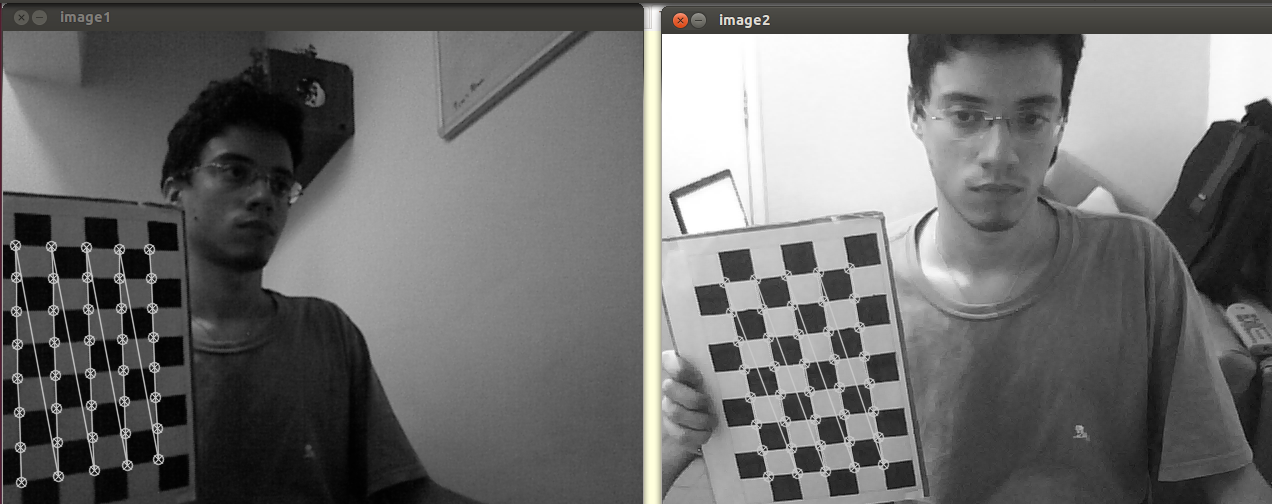
\includegraphics[width=.8\textwidth]{images/kinect2glassesa.png}
  \label{fig:kinect2glassesa}
}
\subfigure[Reconstructed model from Kinect]
{
  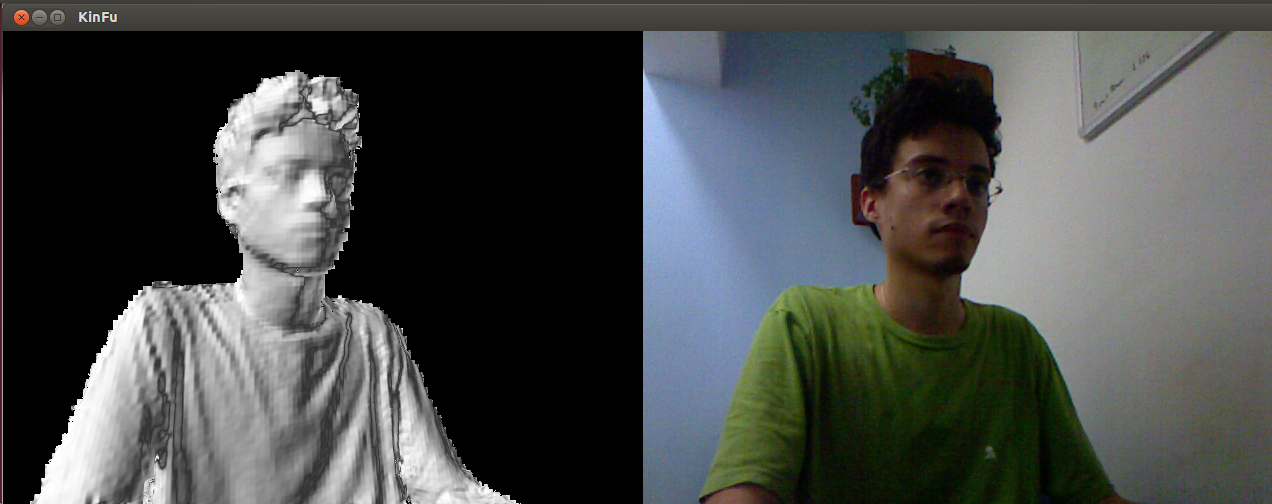
\includegraphics[width=.8\textwidth]{images/kinect2glassesb.png}
  \label{fig:kinect2glassesb}
}
\subfigure[Model captured by Kinect transformed to glasses' camera space according to the calibration between them]
{
  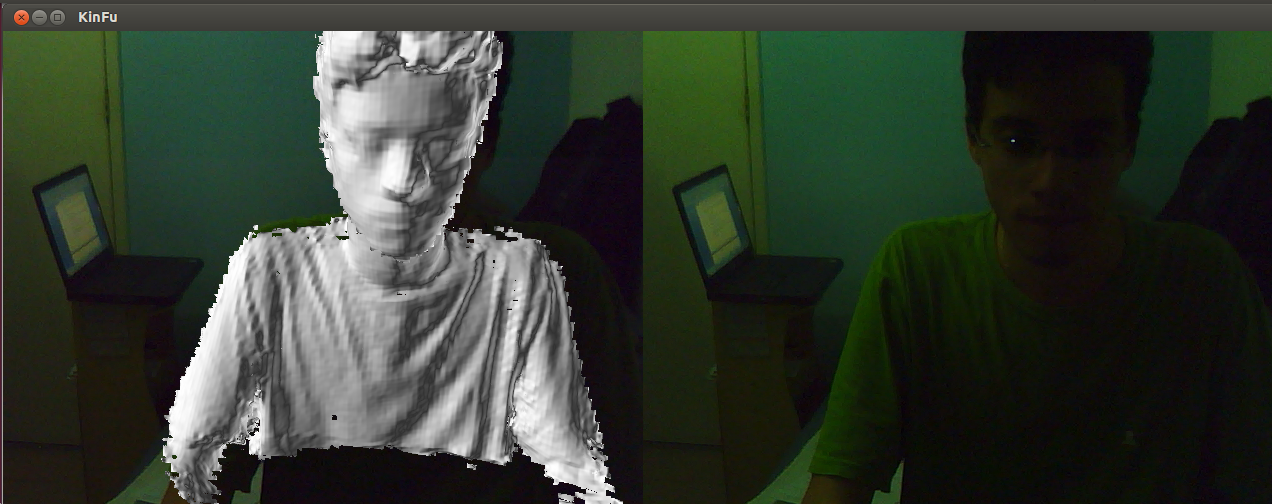
\includegraphics[width=.8\textwidth]{images/kinect2glassesc.png}
  \label{fig:kinect2glassesc}
}
\caption{Calibration process and result}
\label{fig:kinect2glasses}
\end{figure}

\section{Communication}
\label{sec:comm}

As mentioned briefly on section \ref{sec:env}, there wasn't enough USB ports or hubs that could accommodate all devices employed on this augmented reality environment. So it was necessary to use more than one computer, and so data would have to be transfered between computers. There were three devices: two Kinects and one pair of augmented reality glasses. All three devices process video streams (which are heavy to be transfered, regardless the method used). So all three USB ports available on the main computer were used for the video input: one Kinect on each USB hub and the glasses' video input on the remaining USB port of one of the hubs. However, the Kinect takes about 70\% of a single hub (not port) to transmit its data \cite{kinecthacks}, so it was necessary to connect the glasses' video input cable to a USB hub with external power supply and then connect the hub to the remaining USB port in order to deliver enough energy to the glasses.

But there was still the data cable from the glasses, which delivers data from the glasses' tracker. Since there wasn't a free port on the main computer, it was necessary to employ another computer. As explained on section \ref{sec:glasses}, it was implemented on the scope of this work a driver for the glasses that was compatible with Linux machines. It reads the raw data from the glasses, converts them to integer values of yaw, pitch and roll and makes these values available under a virtual device located on \textit{/dev}. In order to make it available to the other machine, it was implemented a new component for the augmented reality system, also available at \cite{masterproject}, that reads the values for yaw, pitch and roll from \textit{/dev/wrap920AR} and sends them over the network.

Since one of the objectives of this work was to run in real-time, velocity was a major concern. At a first glance, there were two main possibilities: connect both computers through a local wireless network or through a local wired network (what would be faster than the wireless approach), but the final decision was to make a cross-over connection between both computers, because is the fastest approach and also doesn't require a network infrastructure, which makes the overall augmented reality environment a bit simpler to be installed and configured. In order to configure the cross-over connection between the two computers, it was necessary to connect the ethernet cross-over cable between both devices (as shown on Figure \ref{fig:cross}) and just run the commands \textit{ifconfig eth0 192.168.1.1 up} on the first computer and \textit{ifconfig eth0 192.168.1.2 up} on the second computer. The \textit{ifconfig} command is a Linux utility to configure network interfaces, while \textit{eth0} is the virtual network interface that identifies the network interface card and the second parameter is the IP. After that, both computers were connected with minimum delay. Table \ref{tab:ping} shows the times to send a packet from one computer to the other through the command line \textit{ping} utility, for each one of the approaches.

\begin{figure}
\centering
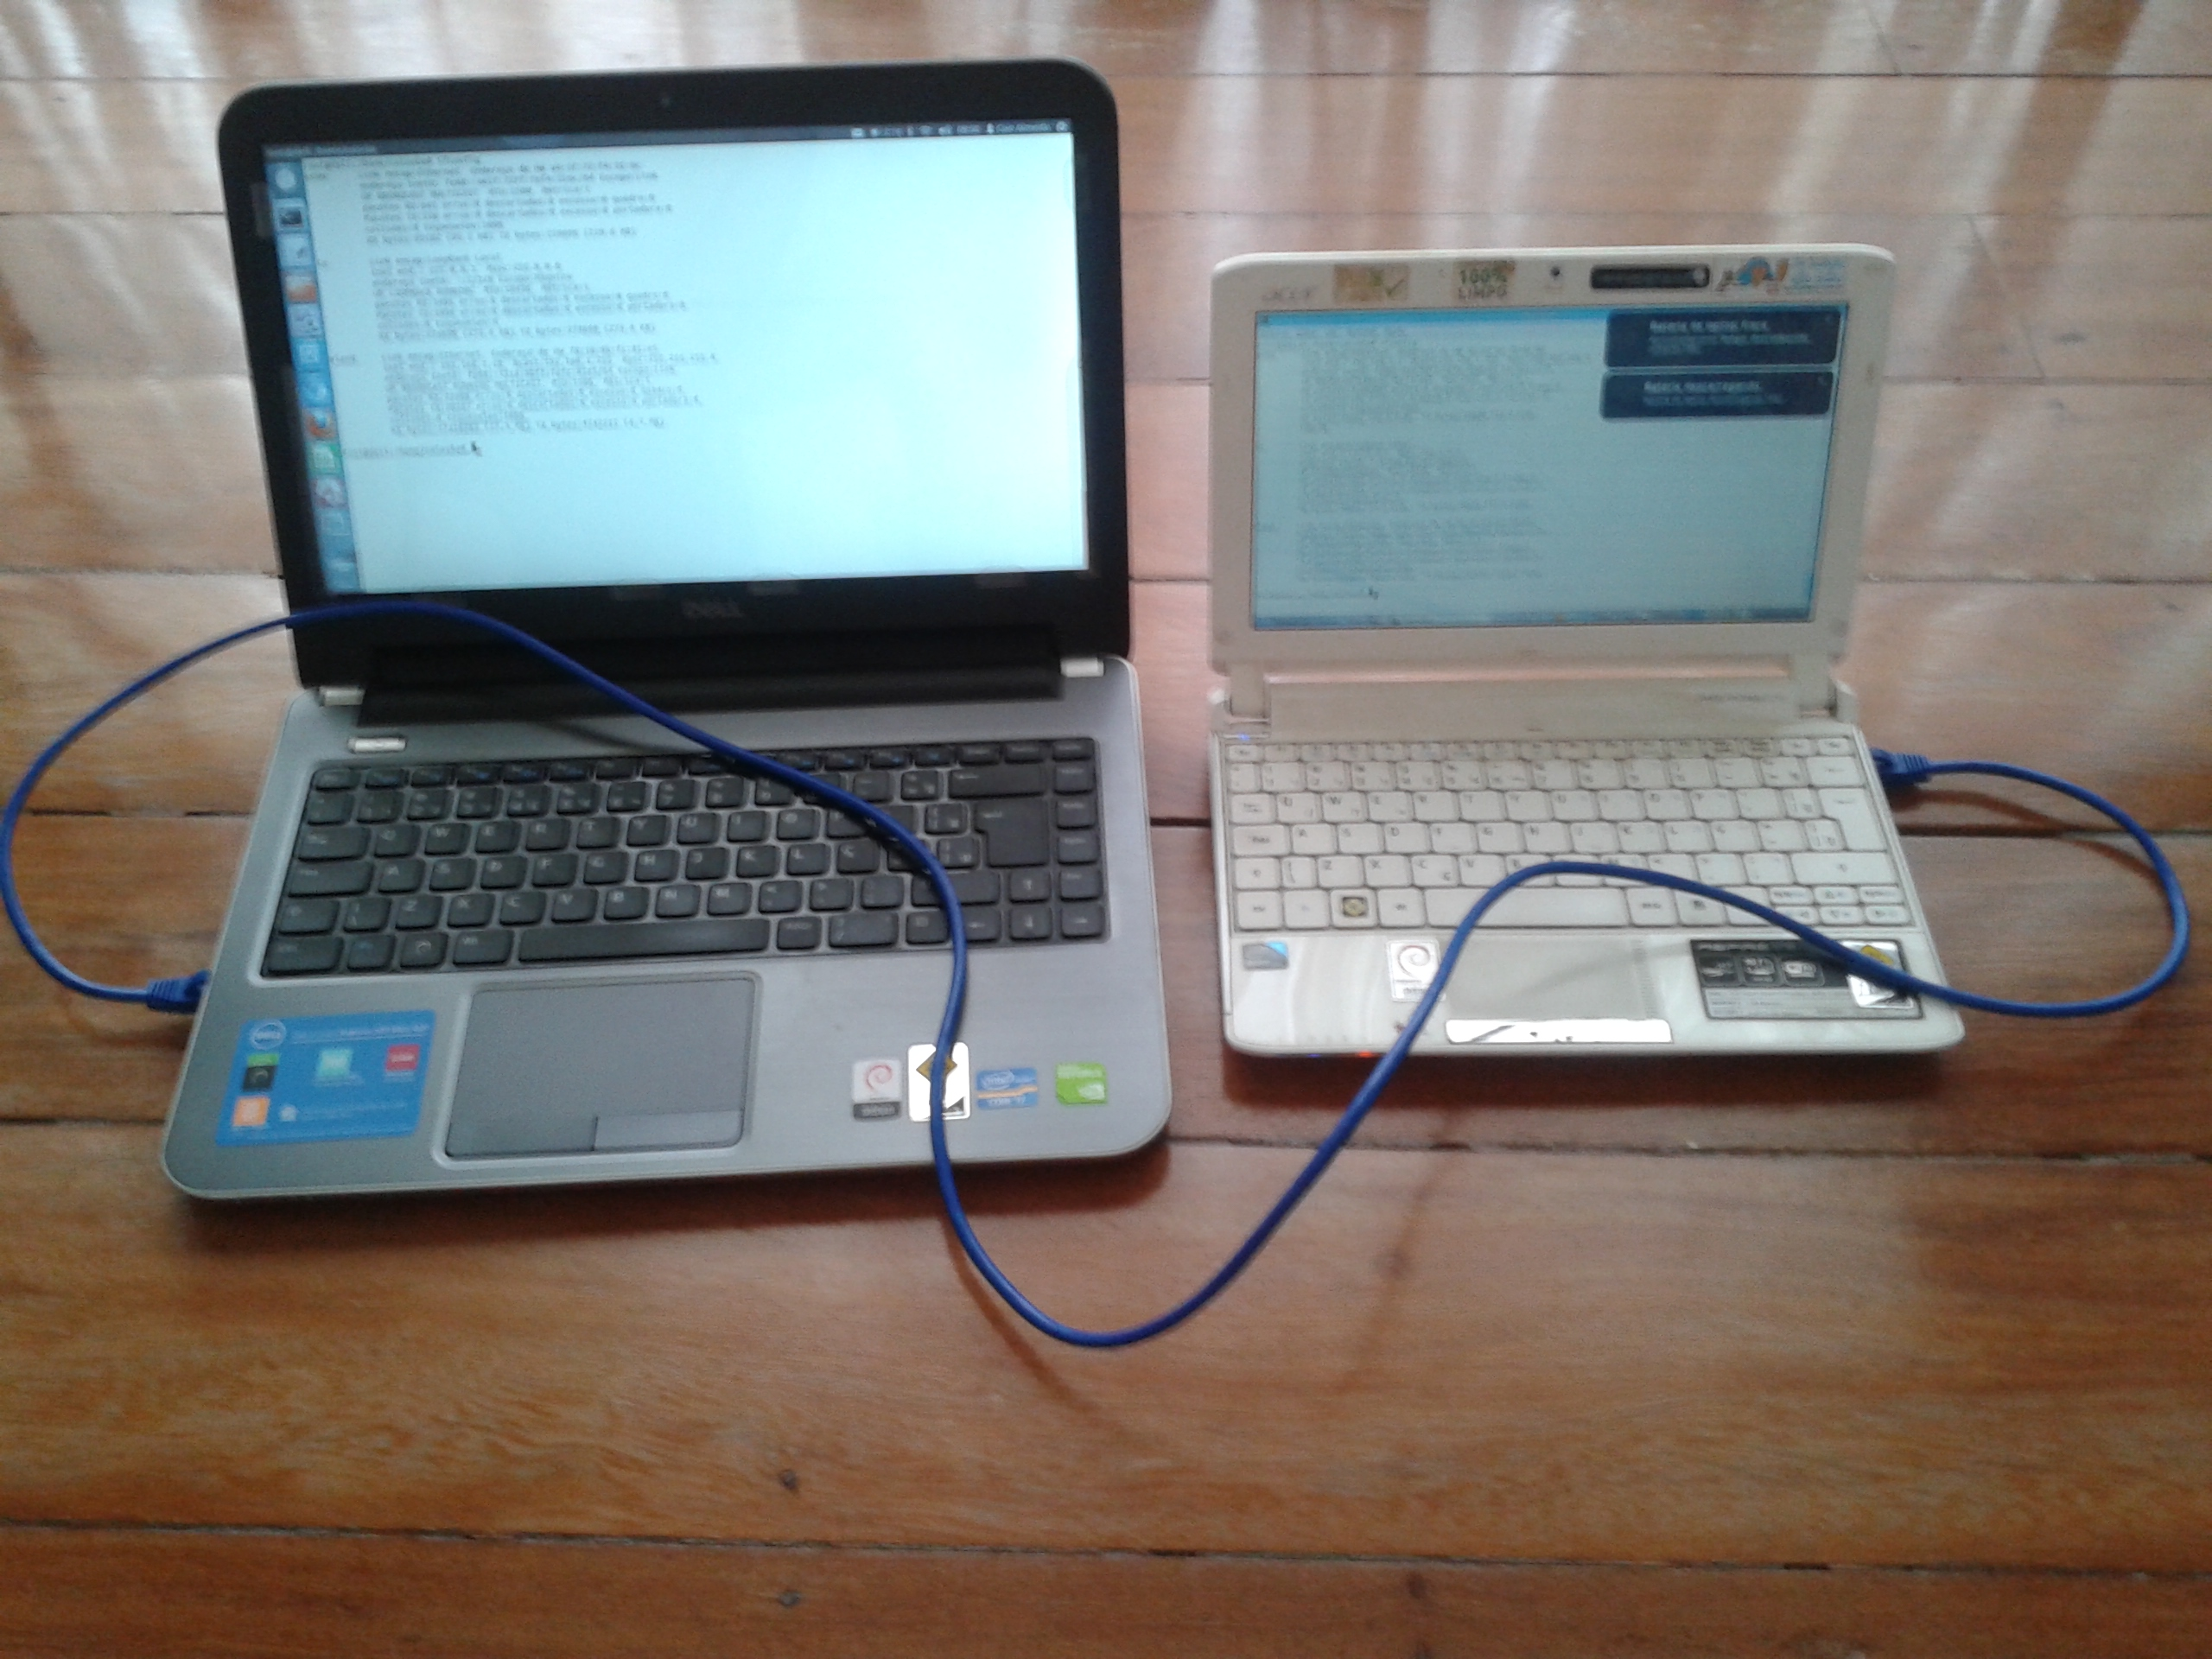
\includegraphics[width=0.5\textwidth]{images/cross.jpg}
\caption{Cross-over connection between two computers}
\label{fig:cross}
\end{figure}

\begin{table}
\caption{Times to send a packet from one computer to other using different network structures}
\label{tab:ping}
\centering
\begin{tabular}{|c|c|c|c|c|c|c|}
\hline
Network type & Packet 1 & Packet 2 & Packet 3 & Packet 4 & Packet 5 & Packet 6 \\
\hline
             & Packet 7 & Packet 8 & Packet 9 & Packet 10 & Average & Maximum \\ 
\hline
Wireless & 97.2 ms & 319 ms & 40.4 ms & 62.7 ms & 85.2 ms & 90.5 ms \\
\hline
         & 27.5 ms & 349 ms & 71.9 ms & 95.0 ms & 124.000 ms & 349.863 ms \\
\hline
Ethernet & 0.849 ms & 0.215 ms & 0.237 ms & 0.199 ms & 0.245 ms & 0.217 ms \\
\hline
         & 0.187 ms & 0.228 ms & 0.184 ms & 0.186 ms & 0.274 ms & 0.849 ms \\
\hline
Cross-over & 0.203 ms & 0.194 ms & 0.196 ms & 0.175 ms & 0.166 ms & 0.168 ms \\
\hline
           & 0.152 ms & 0.173 ms & 0.215 ms & 0.181 ms & 0.182 ms & 0.215 ms \\
\hline
\end{tabular}
\end{table}

Is also worth noticing that on this case the network was dedicated only to this task (there wasn't no any other device on connected to the network, regardless the configuration). So, in a real situation, with more devices competing for packets, the difference from the cross-over connection to the other two could be even higher. It's also possible to notice from Table \ref{tab:ping} that the cross-over approach has the lowest difference between the average and the higher time spent to send a packet, which shows its higher stability.

Once the computers are connected, the glasses were ready to send the values of yaw, pitch and roll to the main computer. Basically there were two protocols here that could be used: TCP or UDP (see Figure \ref{fig:udptcp}). They are not the unique protocols that work at the transport layer of a network, but the most used ones. TCP means \textit{Transmission Control Protocol} and is the most common way to transfer packets over the internet. The biggest feature of TCP is reliability: it manages message acknowledgment, retransmission and timeout. It does multiple attempts to deliver the message and if it gets lost along the way, the server will re-request the lost part. In TCP, there's either no missing data. However, it's also heavier: it requires three packets to setup a socket connection, before any data can be sent \cite{udp}.

\begin{figure}
\centering
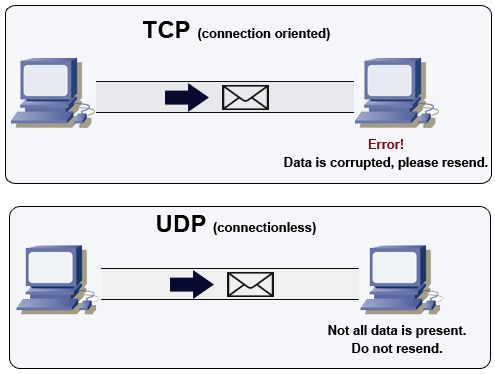
\includegraphics[width=0.5\textwidth]{images/udptcp.png}
\caption{UDP and TCP protocols}
\label{fig:udptcp}
\end{figure}

On the other hand, UDP (which stands \textit{User Datagram Protocol}, uses a simple connectionless transmission model with a minimum protocol mechanism. It's unreliable: when a UDP message is sent, there is no guarantee that it will reach the client, since it can get lost along the way. There is no concept of acknowledgment, retransmission, timeout, ordering or congestion control. However, it is also lightweight: applications can send messages (called \textit{datagrams}) to other hosts without prior communications or special configurations. Time-sensitive applications often use UDP because dropping packets is preferable to waiting for delayed packets, which may not be an option in a real-time system \cite{udp}, like this one.

Since any control is provided by the UDP protocol, on the application that gets the glasses' tracker data an index number and prefix are attached to the datagram, along with the integer values for yaw, pitch and roll. For example, a valid datagram sent by this application through a UDP socket is \textit{GYPR 12 0 32 67}, where \textit{GYPR} (which stands for \textit{Glasses Yaw Pitch Roll}) is a prefix that identifies this packet as one coming from the application, \textit{12} means that this is related to the 12º frame, and \textit{0}, \textit{32} and \textit{67} are the degrees values for yaw, pitch and roll, respectively. Hosts and ports involved on this communication are defined as configuration options for the client and server applications. More details on this application will be explained on the next section \ref{sec:method1}.

\section{Method 1: Glasses accelerometer and one Kinect}
\label{sec:method1}

Once the devices were calibrated and able to communicate, it was time to connect all of them in a single augmented reality environment. On this work we tried two different approaches to track the observer's head movement: by using glasses' data or by using the observer's model as captured by another Kinect device. On this chapter, the former will be explained.

The main component implemented on this approach is based on \textit{MyKinectFusion} \cite{marcio}. \textit{MyKinectFusion} is a fork of \textit{KinFu} that supports augmented reality with polygonal surfaces or medical volumes. So, the merging of virtual images with real ones is handled by this part of the code, while here the goal is to transform the reconstructed and augmented model to the different view points of this multi-view environment. Finally, \textit{KinFu} is an open source implementation of KinectFusion algorithm and is part of the PCL library, but not available on the stable version of PCL (as of version 1.4, the one employed here), but can be found on the repositories of the library. The code is written in C++ and uses the PCL libraries. \textit{KinFu} itself introduces a few modifications to the original KinectFusion algorithm, as can be noticed by reading the source code. KinFu can work with any OpenNI-compatible device, while KinectFusion just works with Kinect, as expected. The normal estimation step is done through eigenvalue estimation instead of simple cross-vector computation. Rendering is done using a marching cubes algorithm instead of ray casting. It's also possible to save the surface meshes and to represent the point clouds \cite{michele}. Basically, the original code used as base here captures and reconstructs a model, in real-time, according to the Kinect's point of view. The fork implemented on this stage of the project is available at \cite{mykinfu} and integrates the reconstruction features of the original KinFu and the augmented reality support of MyKinectFusion with the glasses' tracking data. The new steps performed here, for each frame, in real-time, are:

\begin{enumerate}
  \item Segments the model's head;
  \item Gets the current rotation matrix and translation vector for the reconstructed model as returned by ICP;
  \item Composes this transformation with the transformation given by the calibration of the glasses with the Kinect that captures the target model;
  \item Composes the rotation of this transformation with the rotation given by the glasses' tracker (accelerometer/magnetometer);
  \item Composes the translation of this transformation with the translation given by the optical flow of feature points on glasses' video;
  \item Sets the pose to the final transformation given by the applications of the previous steps;
  \item Renders the transformed model and shows it on the glasses' lenses.
\end{enumerate}

Each step will be explained in details along this chapter.

The first step here was to port the source code of \textit{MyKinectFusion} from Microsoft Windows to GNU/Linux, until it compiled and ran successfully on Ubuntu 12.04 through \textit{optirun} with CUDA support. The next step was to segment the model, and this was achieved by implementing a truncation of the points that are after a defined threshold, which can be configured, but here the value used was 700 millimeters, so any point from the point cloud that is beyond this value is ignored. Since there are the depth maps, the information about the depth of each point is available. On the experimentation phase, the employed doll (as seen on Figure \ref{fig:expenv}) was not rigid enough to keep its head up, so in order to segment its head, a carton was placed behind that and it was implemented a temporary chroma key feature in order to remove the background and then segment the head. The background removal step was removed afterwards, when running with real people.

The full documentation about the source code is available on the appendix, so here only the most important and altered classes and methods will be covered. The \textit{Reconstruction} class is responsible for handling the reconstructed target model captured by the Kinect device and is instantiated when the code starts. The output file of the calibration process described on section \ref{sec:kinect2glasses} is used as an initial alignment to transform the target model to the glasses' point of view. In order to do that, a new method was implemented on the \textit{Reconstruction} class, called \textit{readPoseFromFile}. This method is run for each frame, and looks for a file called \textit{calibration.yml} on the root of code base. Since it is a native format from OpenCV, the values for the rotation matrix and translation vector are naturally read to variables, which are stored in memory (so the file is not opened for reading and unserialized again for the next frames, which improves the performance) and composed of the current rotation and translation of the reconstructed model by applying the following equations:

\begin{center}
$R = R_{current} \times R_{file}^{-1}$
\end{center}

Where $R$ is the final rotation to be applied to the reconstructed model, $R_{current}$ is the current rotation of the model as returned by ICP and $R_{file}^{-1}$ is the inverse of the rotation matrix read from the file. A similar composition is applied to the translation:

\begin{center}
$T = R_{file}^{-1} \times T_{curr} + T_{file}$
\end{center}

Where $T$ is the final translation to be applied to the reconstructed model. $T_{curr}$ is the current translation as returned by ICP and $T_{file}$ is the translation read from the calibration file. A result of this transformation is represented on Figure \ref{fig:kinect2glassesc}.

However, this transformation is from the calibration process, which assumes that the observer doesn't move (since the glasses' camera is static during the calibration). So it's not possible to use only this information to transform the model. In order to track the observer's head, on this approach it's used information from the glasses' tracker, which is explained on section \ref{sec:glasses}. This integration is managed by a new class, called \textit{Glasses}, whose class diagram is represented on Figure \ref{fig:glassesclassdiagram}. A full class diagram of the whole system is available on the appendix.

\begin{figure}
\centering
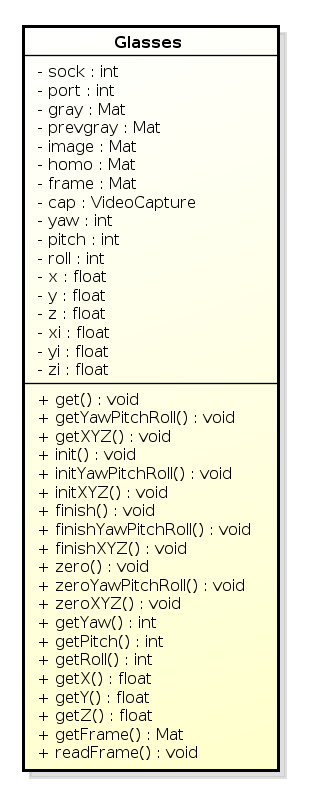
\includegraphics[width=0.2\textwidth]{images/glasses.png}
\caption{Class diagram of \textit{Glasses}}
\label{fig:glassesclassdiagram}
\end{figure}

The role of each attribute and method of this class is briefly described on the lists below:

\begin{itemize}
  \item sock: Stores the instance of the socket used to listen for tracking data that comes from the glasses;
  \item port: The class listens on this port number for incoming tracking data from the glasses;
  \item gray: The grayscale version of the input frame from the glasses, used for optical flow;
  \item prevgray: The grayscale version of the previous frame from the glasses, used for optical flow;
  \item image: A copy from the input frame from the glasses' video;
  \item frame: The actual frame that comes from the glasses' video;
  \item cap: An instance of OpenCV's \textit{VideoCapture} class, which on this case opens and reads the frames from glasses' video stream
  \item yaw: The integer value of the rotation around the yaw axis, as calculated and given by the glasses' tracker;
  \item pitch: The integer value of the rotation around the pitch axis, as calculated and given by the glasses' tracker;
  \item roll: The integer value of the rotation around the roll axis, as calculated and given by the glasses' tracker;
  \item x: The value of the translation on the x axis, as calculated by the optical flow on the glasses' video frame;
  \item y: The value of the translation on the y axis, as calculated by the optical flow on the glasses' video frame;
  \item z: The value of the translation on the z axis, as calculated by the optical flow on the glasses' video frame;
  \item xi: The initial value of the translation on the x axis, as calculated by the optical flow on the glasses' video frame;
  \item yi: The initial value of the translation on the x axis, as calculated by the optical flow on the glasses' video frame;
  \item yi: The initial value of the translation on the x axis, as calculated by the optical flow on the glasses' video frame.
\end{itemize}

\begin{itemize}
  \item get(): Calls the two methods below;
  \item getYawPitchRoll(): Listens on the socket for the values for yaw, pitch and roll and stores them on the respective attributes;
  \item getXYZ(): Executes the Lucas-Kanade algorithm over the current glasses' frame, calculates the translation and stores the values for x, y and z on the respective attributes;
  \item init(): Just calls the two methods below;
  \item initYawPitchRoll(): Opens the socket to communicate with the glasses;
  \item initXYZ(): Opens the glasses' camera and stores to features from the image that will be tracked;
  \item finish(): Just calls the two methods below;
  \item finishYawPitchRoll(): Closes the socket that was being used to communicate with the glasses;
  \item finishXYZ(): Closes the video stream and clear the feature points that were being tracked;
  \item zero(): Just calls the two methods below;
  \item zeroYawPitchRoll(): Sets the values for yaw, pitch and roll as zero;
  \item zeroXYZ(): Sets the values for x, y and z as zero;
  \item getYaw(): A getter for the yaw attribute;
  \item getPitch(): A getter for the pitch attribute;
  \item getRoll(): A getter for the roll attribute;
  \item getX(): A getter for the x attribute;
  \item getY(): A getter for the y attribute;
  \item getZ(): A getter for the z attribute;
  \item readFrame(): Reads the current frame from the glasses' stream and stores it on the respective attribute;
  \item getFrame(): A getter for the frame attribute.
\end{itemize}

When the program starts, a new instance of the \textit{Glasses} class is created, which connects to the UDP socket at the host and port defined on the configuration file. On this host (which on the implementation here is another computer, connect to main one though a cross-over network), there is a program that runs and reads the yaw, pitch and roll values as calculated by the implemented driver. Those values are sent, every 100ms, to a UDP socket. The datagram just consists of a prefix, that identifies the datagram as valid, an index and the integer values for yaw, pitch and roll. It's a very light program that just needs a few resources, and also transfers a tiny datagram, that usually will have a few dozens of bytes. The frames are numbered before being sent, so the main code knows if some frame is missed, but currently does nothing on such case. Details on that were explained on section \ref{sec:glasses}.

Back to the core program, after an instance of the \textit{Glasses} class is created, a new thread, separated from the main one, is triggered. The library used for managing the threads here is the popular \textit{pthreads} \cite{pthreads}, a set of C language programming types and procedure calls for creating and manipulating threads, as defined by a POSIX standard. This thread runs indefinitely, with an interval of 100ms between consecutive iterations. On each iteration, this thread listens on the UDP socket for new datagrams that contain the values for yaw, pitch and roll and stores them on the respective attributes of the \textit{Glasses} instance that was created.

It's worth noticing that, as stated on the manufacturer's manual \cite{vuzixsdk}, the employed model of the glasses and its SDK version don't support all the six degrees of freedom, so it's only possible to get accurate values for yaw, pitch and roll from the tracker. So, in order to provide the values for translation motion along the x, y and z axes, an optical flow approach was implemented. This also happens on the glasses' thread.

The glasses' thread is also responsible, on each iteration, for reading a frame from the glasses' video stream and for executing the optical flow algorithm over it. The algorithm implemented here is the pyramidal version of Lucas-Kanade one, explained on section \ref{sec:lucas}. On the first run, on the main thread, it tracks the key features of the image, which is done automatically by using Shi-Tomasi algorithm, also cited on section \ref{sec:lucas}. The Shi-Tomasi method will try to find corners on the grayscale version of frame, by performing the following steps:

\begin{enumerate}
  \item Calculates the corner quality measure at every source image pixel and stores this information on a \textit{qualityMeasureMap};
  \item Performs a non-maximum suppression (the local maximums in a 3x3 neighborhood are retained);
  \item The corners with the minimal eigenvalue less than $0.01 \times MAX(qualityMeasureMap)$ (1\% of the best corner quality measure) are rejected;
  \item The remaining corners are sorted by the quality measure in descending order;
  \item Corners for which there is a stronger corner at a distance less than the maximum distance are rejected as well.
\end{enumerate}

After that, the key points for the frame are stored and can be tracked on the next frames by the pyramidal Lucas-Kanade algorithm, as shown on Figure \ref{fig:lk}. The OpenCV's \textit{cornerSubPix} is also employed here in order to get a better accuracy for the coordinates of the feature points that were identified.

\begin{figure}
\centering
\subfigure[Features automatically detected by Shi-Tomasi method (green dots)]
{
  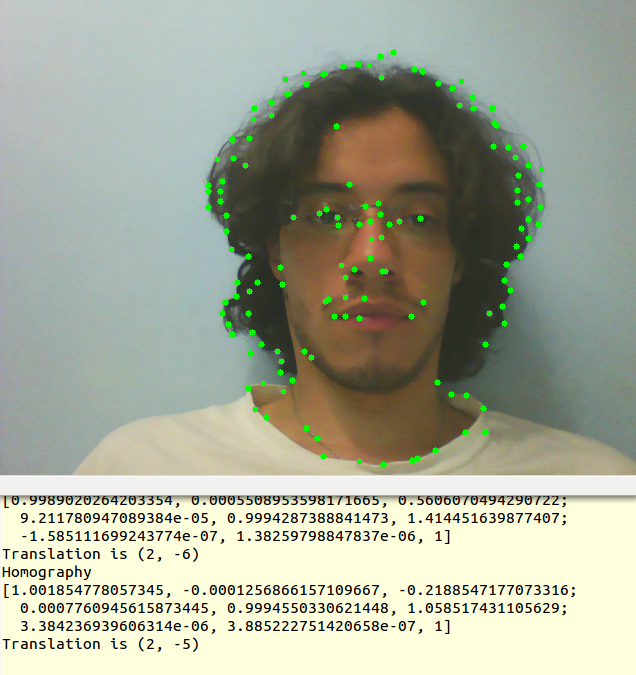
\includegraphics[width=.3\textwidth]{images/lk1.png}
  \label{fig:lk1}
}
\subfigure[Face tracking by Pyramidal Lucas-Kanade, moving to the left]
{
  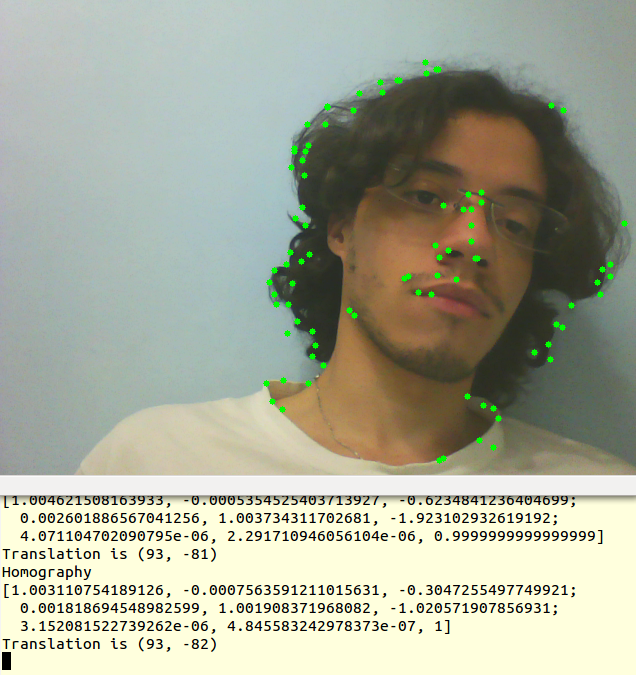
\includegraphics[width=.3\textwidth]{images/lk2.png}
  \label{fig:lk2}
}
\subfigure[Face tracking by Pyramidal Lucas-Kanade, moving to the right]
{
  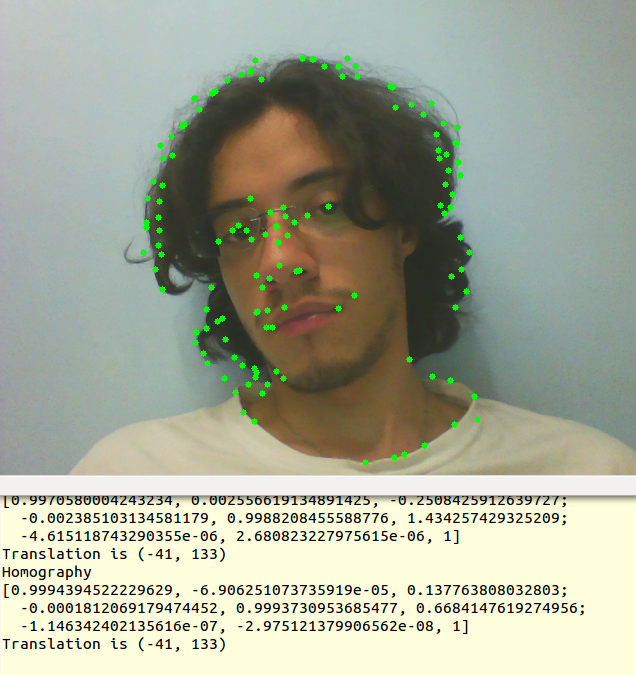
\includegraphics[width=.3\textwidth]{images/lk3.png}
  \label{fig:lk3}
}
\caption{Lucas-Kanade algorithm tracking a face whose key points were previously identified through Shi-Tomasi algorithm}
\label{fig:lk}
\end{figure}

Back to the glasses' thread, on each iteration, pyramidal Lucas-Kanade algorithm is used for tracking that feature points that were previously identified. The previous point set and previous grayscale frame are stored for comparison. After Lucas-Kanade method runs, there will be the previous and current grayscale frames as well as the feature points identified on each. Once the two feature points sets are available, the homography between them is calculated, which will find the perspective transformation between the current and the previous feature points, thus defining the approximate translation performed by the observer.

The homography matrix (denoted below by $H$) relates the positions of the points in the previous frame (source) with the points on the current frame (destiny) by the following equations \cite{bradski2008learning} so that the back-projection error is minimized.

\begin{center}
$P_{dst} = H \times P_{src}, P_{src} = H^{-1} \times P_{dst}$
\end{center}

\begin{center}
$P_{dst} = \begin{bmatrix} x_{dst} \\ y_{dst} \\ 1 \end{bmatrix}, P_{dst} = \begin{bmatrix} x_{src} \\ y_{src} \\ 1 \end{bmatrix}$
\end{center}

However, if not all of the point pairs fit the rigid perspective transformation (that is, there are some outliers), this initial estimate will $H$ be poor. Here it uses the RANSAC method, which tries many different random subsets of the corresponding point pairs (of four pairs each), to estimate the homography matrix using this subset and a simple least-square algorithm, and then compute the quality/goodness of the computed homography (which is the number of inliers for RANSAC). The best subset is then used to produce the initial estimate of the homography matrix and the mask of inliers/outliers. After that, the translation values for x, y and z are extracted from the matrix and returned. The current grayscale frame becomes the previous grayscale frame, the current feature points set becomes the previous feature points set and so the algorithm iterates for the next frames. Since the values for x, y and z are related to the transformation between the current and previous frames and the interest here is on the transformation between the current frame and the first frame, the values for x, y and z are always accumulated instead of replaced.

After connecting to the socket and performing the optical flow over the glasses' frame, the values for yaw, pitch, roll, x, y and z are already available and set as attributes of the \textit{Reconstruction} object, which is shared between the main thread and the glasses thread.

On the main thread of the program, each frame is processed each 100 ms as well. Besides composing the current rotation with the rotation from the calibration file, and the translation with the translation from the calibration, as explained previously, both are also composed with the rotation and translation that come from the glasses.

For yaw, pitch and roll, first it's necessary to convert from Euler angles to matrices. Since the goal here is to transform the model based on the observer's motion, the negative values for each angle will be used. The matrices are:

% Yaw: Y
\begin{center}
$R_{yaw} = \begin{bmatrix}
           \cos(\phi) & \sin(\phi) & 0 \\
           -\sin(\phi) & \cos(\phi) & 0 \\
           0 & 0 & 1 \\
           \end{bmatrix}$
\end{center}

% Pitch: X
\begin{center}
$R_{pitch} = \begin{bmatrix}
             \cos(\theta) & 0 & -\sin(\theta) \\
             0 & 1 & 0 \\
             \sin(\theta) & 0 & \cos(\theta) \\
             \end{bmatrix}$
\end{center}

% Roll: Z
\begin{center}
$R_{roll} = \begin{bmatrix}
            1 & 0 & 0 \\
            0 & \cos(\psi) & \sin(\psi) \\
            0 & -\sin(\psi) & \cos(\psi) \\
            \end{bmatrix}$
\end{center}

Then the current model rotation is compounded with the rotation given by the multiplication of the three matrices above:

\begin{center}
$R_{glasses} = R_{roll} \times R_{pitch} \times R_{yaw} \therefore R =  R_{glasses} \times R_{current}$
\end{center}

The model's translation is given by:

\begin{center}
$T_{glasses} = [x, y, z] \therefore T = R_{glasses} \times T_{current} - T_{glasses}$
\end{center}

After that, the final transformation given by the rotation $R$ and the translation $T$ is applied to the model.

The glasses' tracker is very sensible and can suffer interference from magnetic objects near it \cite{vuzixsdk}, while the optical flow needs at least four feature points in order to keep the tracking \cite{opencvfd}, and most feature points can easily disappear when a fast movement happens. In order to try to mitigate those problems, a new approach was implemented, which uses a second Kinect to calculate the observer's movement, which will be explained on the following section \ref{sec:method2}.

\section{Method 2: Two Kinects}
\label{sec:method2}

On this approach, the only information that's still used from the glasses is the video stream, which is combined with the reconstructed target model. This approach uses the same code as the main component, but on the configuration file the options for glasses' tracking (from both accelerometer/magnetometer and optical flow) are turned off, while the option for using the second Kinect is turned on.

A new component was implemented here, which is called \textit{MyKinFuHeadless}, available at \cite{mykinfuheadless}. It's a simplified version of \textit{MyKinFu} that just captures an object, segments it (removes background or other objects based on the depth map), calculates its transformation from the initial pose and sends this transformation, as a serialized rotation matrix and serialized translation vector, to a UDP socket, in real-time.

The code behaves just like the original \textit{KinFu}. The main difference is that on the original version the ICP calculates the transformation from the current model in relation to the previous one, while here it's necessary to know the transformation from the current model to the initial one. As explained on section \ref{sec:icp}, it takes some iterations until ICP is able to segment the model and ignore new objects that appear on the scene. At this moment, this transformation is considered the initial one. For the next iterations of ICP, it composes the current rotation and current translation and a new calculation introduced here will provide the difference $R_{diff}$ between the current rotation $R_{curr}$ and the initial rotation $R_{ini}$ and the difference $T_{diff}$ between the current translation $T_{curr}$ and the initial translation $T_{ini}$, both given by:

\begin{center}
$R_{diff} = R_{curr} \times R_{ini}^T$
\end{center}

\begin{center}
$T_{diff} = T_{curr} - T_{ini}$
\end{center}

After $R_{diff}$ and $T_{diff}$ are computed, they are sent to a UDP socket as serialized data, since only strings can be written to the socket. Similarly to what was done with the glasses' tracker, on this case an auxiliary code to check the tracker's accuracy was implemented too, and is available at \cite{masterproject}. This auxiliary code uses OpenGL and listens on the same socket where \textit{MyKinFuHeadless} writes to, and transforms the virtual cube as it was seen by the glasses. Figure \ref{fig:secondkinecttrack} shows this accuracy using a box as the observer. Since the geometry of the box is not as irregular as a human head, better results can be achieved on real situations, but it still has a reasonable accuracy.

\begin{figure}
\centering
  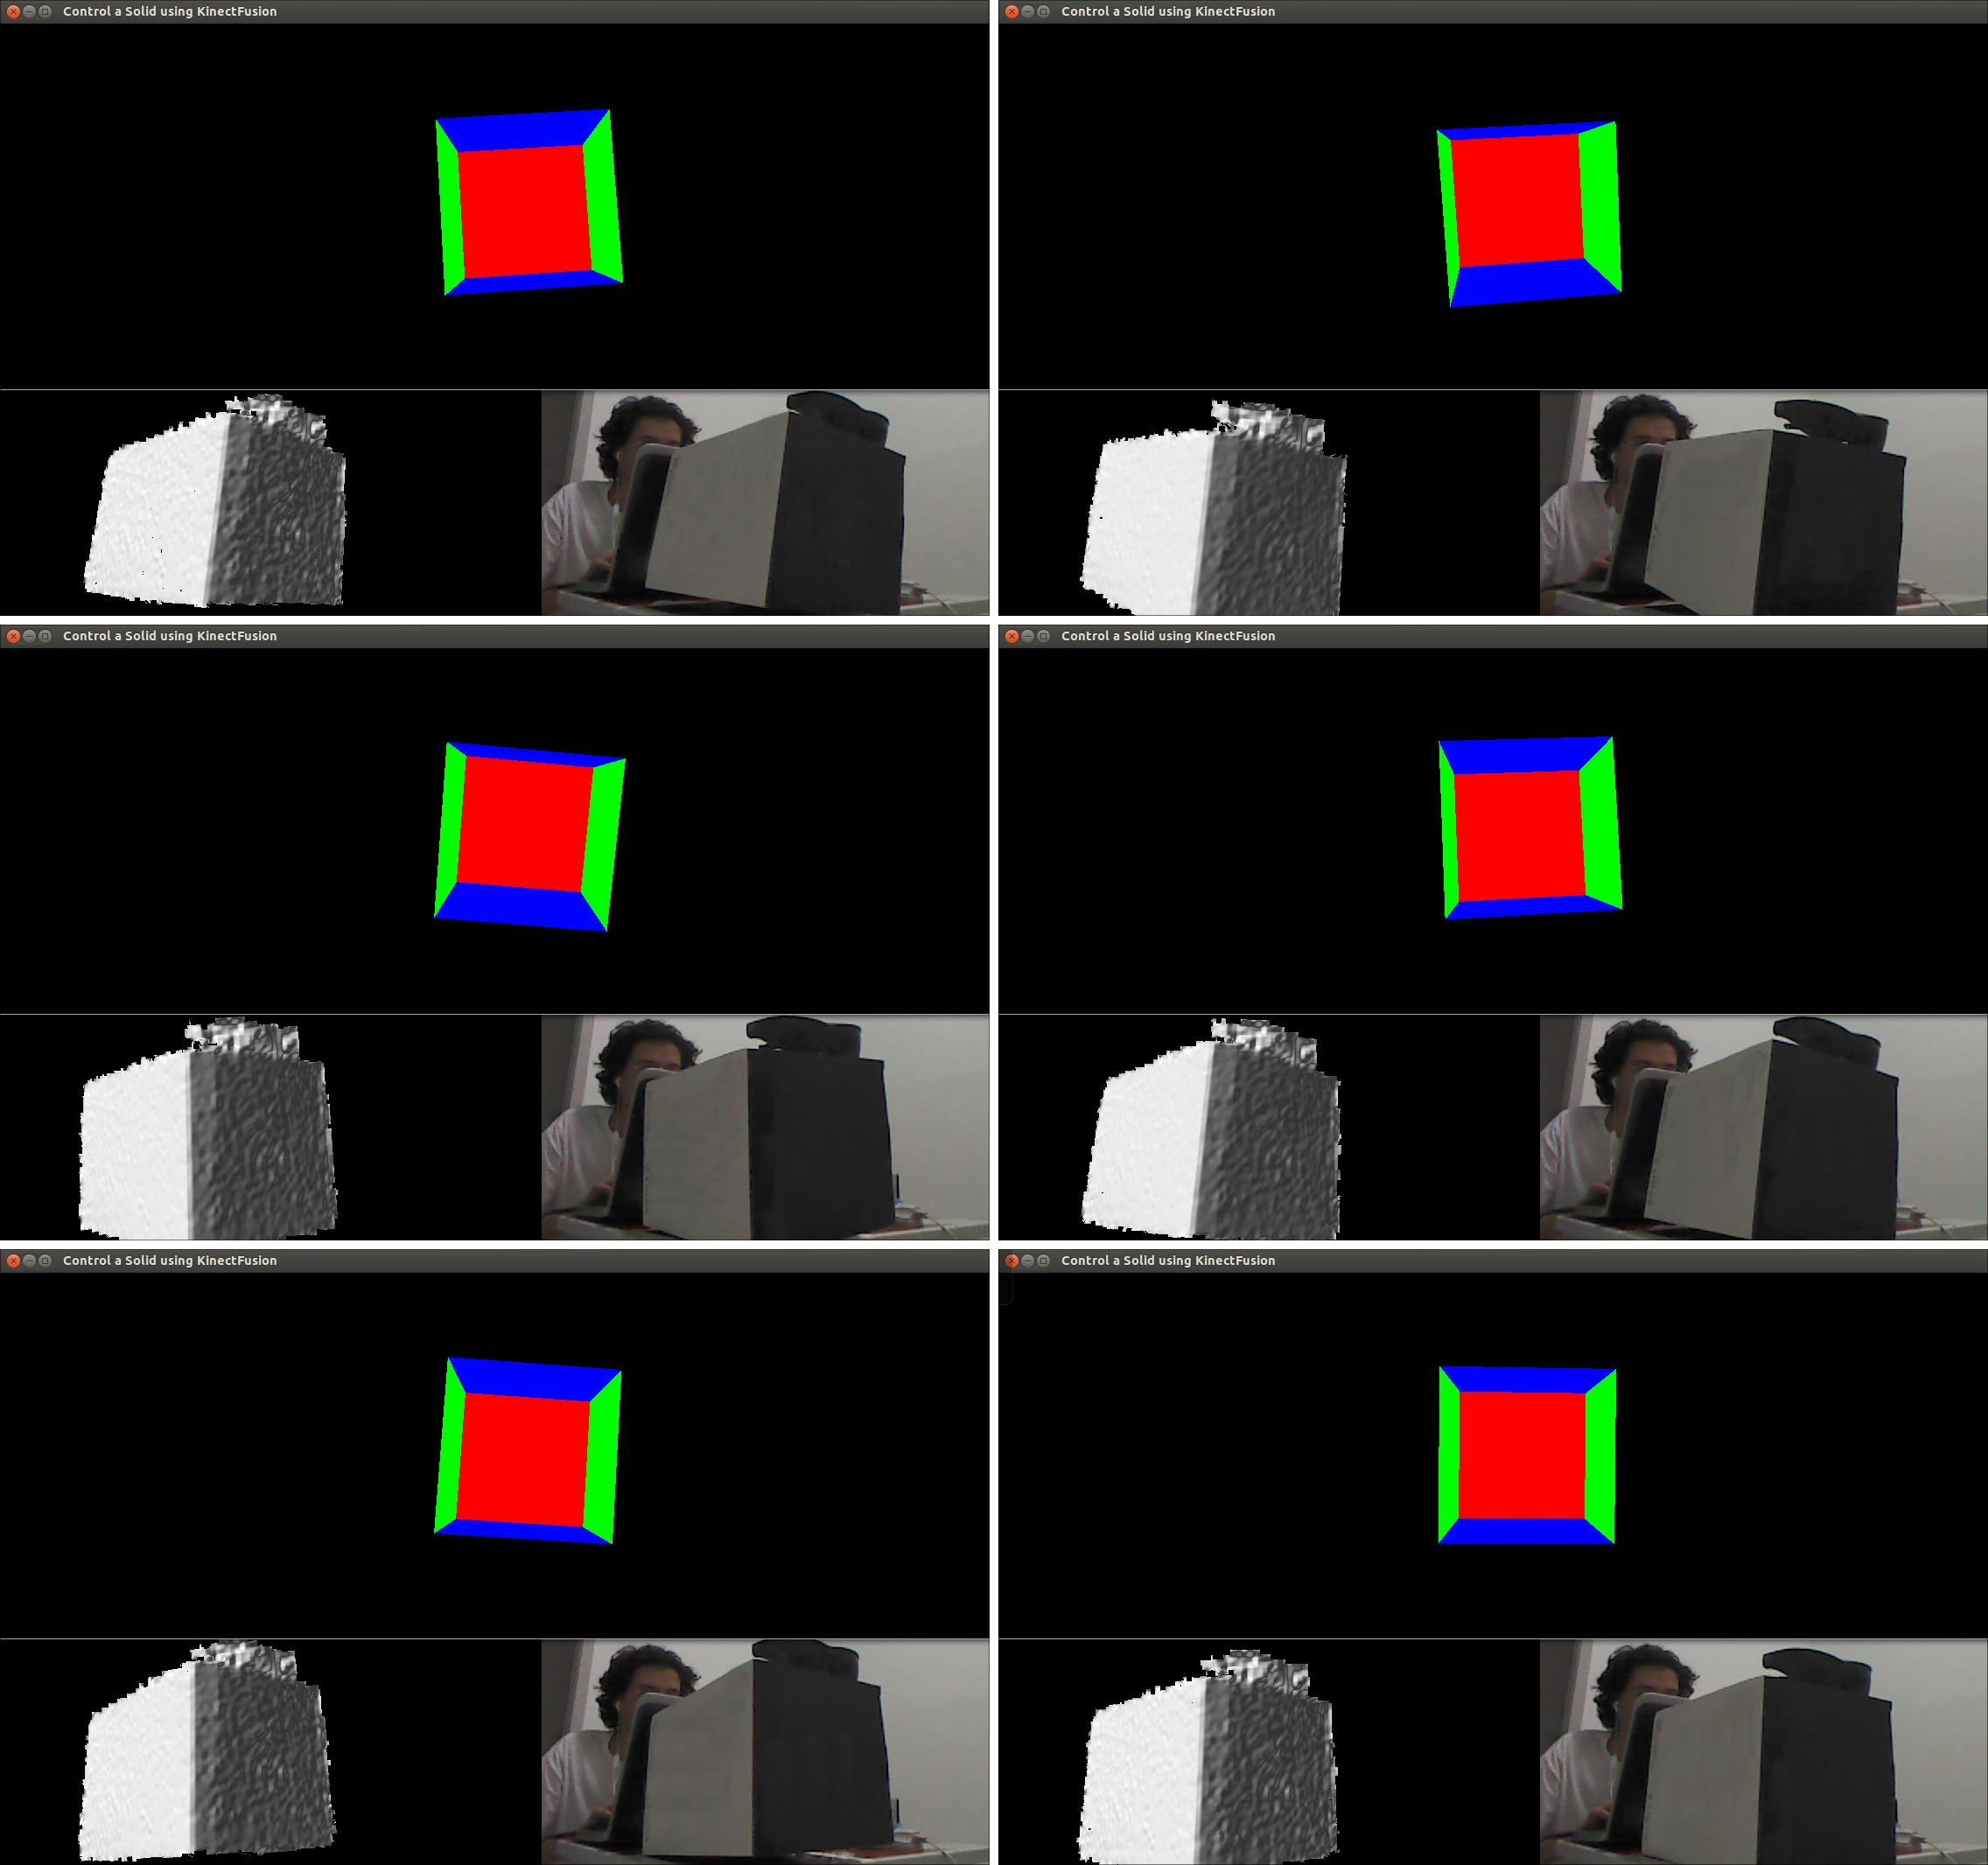
\includegraphics[width=0.5\textwidth]{images/secondkinectrack.png}
\caption{Virtual cube as seen by the observer according to the transformation given by the Kinect that captures it}
\label{fig:secondkinecttrack}
\end{figure}

On the main code side, the change is similar to the one implemented for the first method. A new thread is triggered when the code starts and runs in parallel to the main thread. This thread listens on the UDP socket and gets the rotation matrix and translation vector that represent the transformation of the observer. The values are unserialized and saved with the \textit{Reconstruction} object, which is shared with the main thread. On the main thread, for each frame, the current rotation and translation of the target model are composed with the rotation and translation of the observer as given by the second Kinect, the following way:

\begin{center}
$R = R_{diff} \times R_{curr}$
\end{center}

\begin{center}
$T = T_{curr} + [T_{diff_x}, -T_{diff_y}, T_{diff_z}]$
\end{center}

As explained on section \ref{sec:kinfu}, it needs CUDA to run, and on this experimental augmented reality environment there was only one computer with a graphics card with CUDA support. The \textit{MyKinFuHeadless} component is a standalone code that sends the calculated values to a socket, so it could (and actually should) run on a separate machine, since two programs that needs the GPU running on the same machine would decrease the overall performance.

But since there was only one computer with CUDA support, it would be necessary to run \textit{MyKinFu} and \textit{MyKinFuHeadless} on the same machine at the same time. A benchmark showed that each of them running separately took approximately 90 ms to process one frame. When both were running at the same time, this value jumped to approximately 180 ms, which makes sense, since both were fighting for a single GPU. The result was a huge delay between the observer's real movement and the respective virtual transformation on the rendered frame. So it was necessary to improve the performance. A more detailed benchmark showed that most of the time was spent on ICP and point clouds alignment:

\begin{verbatim}
setDepthDevice took 0ms.
setRgbDevice took 0ms.
applyBilateralFilter took 0ms.
applyDepthTruncation took 0ms.
applyPyrDown took 0ms.
convertToPointCloud took 20ms.
applyDepthTruncation took 0ms.
sync took 0ms.
ICP level 2 iteration 0 took 0ms.
ICP level 2 iteration 1 took 0ms.
ICP level 2 iteration 2 took 8ms.
ICP level 2 iteration 3 took 8ms.
ICP level 1 iteration 0 took 9ms.
ICP level 1 iteration 1 took 9ms.
ICP level 1 iteration 2 took 9ms.
ICP level 1 iteration 3 took 9ms.
ICP level 1 iteration 4 took 26ms.
ICP level 0 iteration 0 took 31ms.
ICP level 0 iteration 1 took 7ms.
ICP level 0 iteration 2 took 7ms.
ICP level 0 iteration 3 took 7ms.
ICP level 0 iteration 4 took 7ms.
ICP level 0 iteration 5 took 7ms.
ICP level 0 iteration 6 took 7ms.
ICP level 0 iteration 7 took 7ms.
ICP level 0 iteration 8 took 7ms.
ICP level 0 iteration 9 took 7ms.
alignPointCloud took 96ms.
reset took 0ms.
integrateVolume took 24ms.
raycast took 37ms.
last sync took 0ms.
last step took 1ms.
TOTAL FRAME took 184ms.
\end{verbatim}

The first step was to change the virtual volume size of KinectFusion, which is by default 3000 mm x 3000 mm x 3000 mm, because it's intended to be used to scan large scenarios. Since the use case here is just faces, it's not necessary to use such dimensions for the volume size. It was changed to 700 mm x 700 mm x 1400 mm and the voxel size from 512 to 256 per axis (both the number of voxels and the size in meters give the amount of detail of our model) and the result was still satisfactory. See Figure \ref{fig:kinfu} to better understand the virtual cube of KinectFusion.

\begin{figure}
\centering
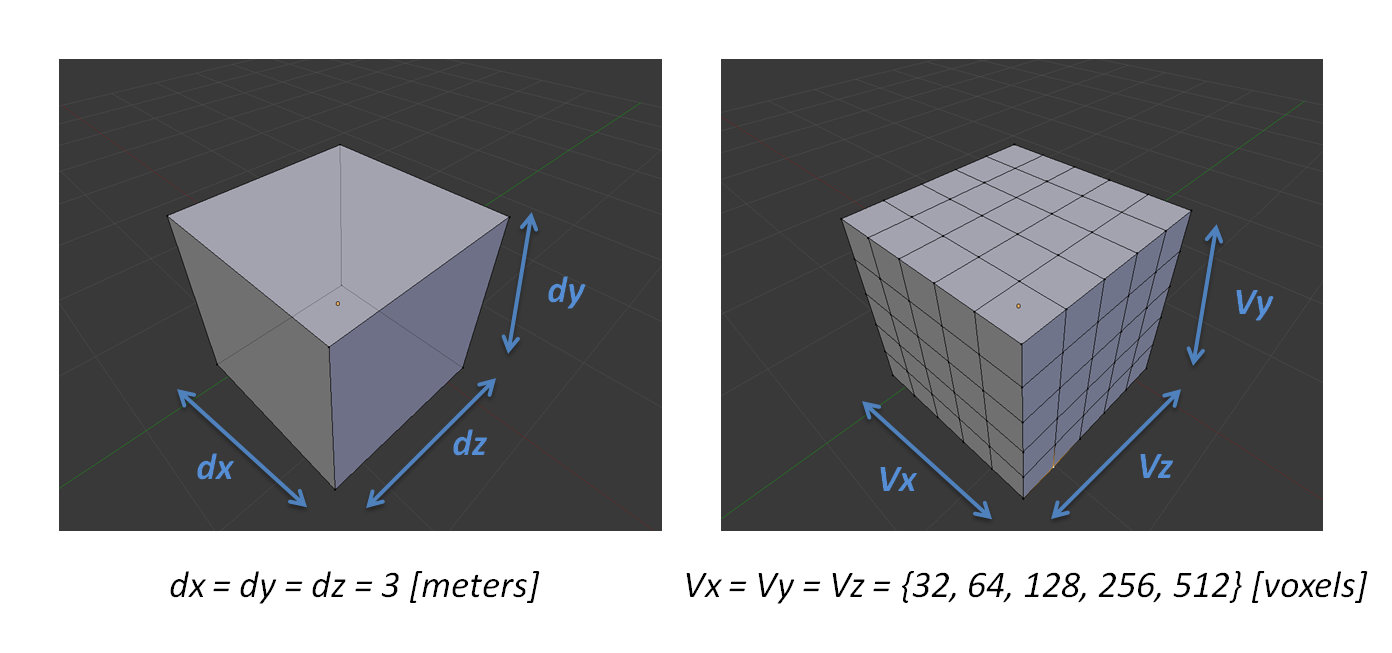
\includegraphics[width=1\textwidth]{images/kinfu.jpg}
\caption{The cube is subdivided into a set of voxels; these voxels are equal in size; the default size in meters for the cube is 3 meters per axis; and the default voxel size is 512 per axis \cite{pclkinfu}}
\label{fig:kinfu}
\end{figure}

Also, the number of ICP iterations were reduced, and since it was one of the most time-consuming steps, the overall runtime was decreased. As a last step, the code was refactored to use the most recent libraries, using as reference another refactoring of KinFu called \textit{KinFuRemake} \cite{kinfuremake}. The result was a code twice faster (see chart at Figure \ref{fig:kinfuchart}). Thus, now, \textit{MyKinFu} and \textit{MyKinfuHeadless} running at the same time on the same machine was consuming the same time as just one of them was consuming alone previously.

\begin{figure}
\centering
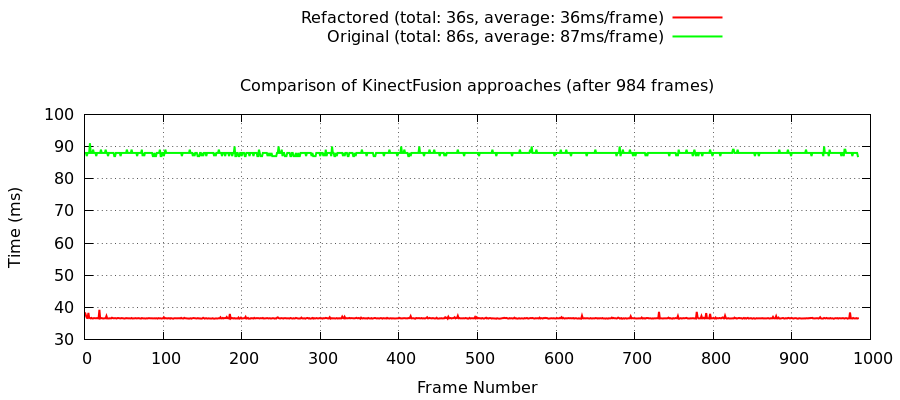
\includegraphics[width=1\textwidth]{images/plot.png}
\caption{Comparison of time to process a frame before and after the refactoring}
\label{fig:kinfuchart}
\end{figure}

This approach has shown to be visually better for greater range of motion, although the accuracy was not that good for simpler movements and the performance was much worse. In order to combine the best of the two approaches implemented on this work, an hybrid approach was proposed, which will be explained on the following section \ref{sec:hybrid}.

\section{Hybrid approach}
\label{sec:hybrid}

The hybrid approach is just a combination of the two previous methods. On this approach, both threads (one for the glasses and the other for the Kinect that captures the observer) are kept running simultaneously. The glasses' data are used primarily since it has better performance. If the number of tracked features for the optical flow goes below eight points, the transformation calculated by the second Kinect is used in order to transform the target model. This method has the best accuracy since it applies each method to the situation they fit better. The results of running each of the three methods with real people will be shown on the next section \ref{sec:results}.

\xchapter{Result}{In this chapter I present the results of the procedure explained in the previous chapter.}
\label{sec:results}
\section{Scope}
Talk about error propagation.
\section{Analysis}
Talk about performance and alignment results.
\section{Comparison}
Compare methods 1 and 2 with regards to performance and quality.

\xchapter{Conclusions}{In this chapter I discuss the conclusions of this work and list some possibilities of future works.}
\section{Future work}

\backmatter

% Apêndices
% Comente se não houver apêndices
\appendix

% É aconselhável criar cada apêndice em um arquivo à parte, digamos
% "apendice1.tex", "apendice.tex", ... "apendiceM.tex" e depois
% incluí-los com:
% \include{apendice1}
% \include{apendice2}
% ...
% \include{apendiceM}


% Bibliografia
% É aconselhável utilizar o BibTeX a partir de um arquivo, digamos "biblio.bib".
% Para ajuda na criação do arquivo .bib e utilização do BibTeX, recorra ao
% BibTeXpress em www.cin.ufpe.br/~paguso/bibtexpress
\bibliographystyle{abnt-alf}
\bibliography{template}

%% Fim do documento
\end{document}
